\documentclass[11pt,a4paper]{article}

\usepackage{amsfonts,amsmath,amssymb}
\usepackage[margin=1in]{geometry}
\usepackage[none]{hyphenat}
\usepackage{graphicx}
\usepackage{fancyhdr}
\usepackage{float}
\usepackage{color}
\usepackage{xcolor}
\usepackage{tikz}
\usepackage{multirow}

\usepackage[nottoc,notlot,notlof]{tocbibind}

\usetikzlibrary{arrows.meta,shapes,trees,positioning,calc}

\parindent 0ex
\setlength{\parskip}{0.55\baselineskip}
% Displays carry their own skips; with a non-zero \parskip on top of them,
% consecutive displays drift apart. Tighten them so the page reads as argument
% rather than as a list of disconnected formulae.
\setlength{\abovedisplayskip}{0.5\baselineskip}
\setlength{\belowdisplayskip}{0.5\baselineskip}
\setlength{\abovedisplayshortskip}{0.25\baselineskip}
\setlength{\belowdisplayshortskip}{0.25\baselineskip}

\pagestyle{fancy}
\fancyfoot[C]{{page} \thepage}
\fancyhead{}
\fancyhead[R]{\rightmark}

% Theorem environments. The source declared none: all 273 results were set as
% bold text with the number typed by hand, so nothing was numbered by LaTeX,
% nothing could be cross-referenced, and a result inserted anywhere meant
% renumbering the rest of the section by hand.
\usepackage{amsthm}
\theoremstyle{definition}
% The source numbered section.subsection.n from one counter shared by
% definitions, theorems and examples alike (1.1.1 Definition, 1.1.2 Definition,
% 1.1.3 Example, ...). That scheme is kept, so the numbering a reader of the
% original would recognise survives. Notes and remarks stay unnumbered because
% they interrupt rather than advance the argument.
\newtheorem{thm}{Theorem}[subsection]
\newtheorem{defn}[thm]{Definition}
\newtheorem{exa}[thm]{Example}
\newtheorem{prop}[thm]{Proposition}
\newtheorem{coro}[thm]{Corollary}
\newtheorem{lem}[thm]{Lemma}
\newtheorem{result}[thm]{Result}
\newtheorem*{note}{Note}
\newtheorem*{remark}{Remark}
\newtheorem{problemx}{Problem}[section]
\newenvironment{problem}{\begin{problemx}}{\end{problemx}}
\newenvironment{solution}
  {\renewcommand{\qedsymbol}{}\begin{proof}[\textit{Solution}.]}
  {\end{proof}}
\usepackage{enumitem}
% A heading that is legal inside a theorem body, a list or a float, where
% \subsubsection is not. Same weight as \subsubsection* so the two read alike.
\newcommand{\subhead}[1]{%
  \par\medskip\noindent\textbf{#1}\par\nobreak\smallskip}

\begin{document}

% Title page depersonalised for the web, as with every other course here: no
% university crest, no author, no year. The identity kept below is the
% eigenvalue equation, which the second half of the course is an elaboration of.
\begin{titlepage}
\begin{center}
\vspace*{3cm}
{\Huge\bfseries Linear Algebra}\\[1.2cm]
{\large Lecture Notes}\\[2.5cm]
\line(1,0){300}\\[1.5cm]
$$A\underline{x} = \lambda\underline{x}$$
\end{center}
\end{titlepage}

\tableofcontents
\thispagestyle{empty}
\clearpage
\setcounter{page}{1}

\pagebreak

\section{PRELIMINARIES}
\subsection{Sets}
\begin{defn}
A \emph{set} is a well defined collection of objects, called the
\emph{elements} or \emph{members} of the set. We write $x\in X$ to say that $x$
is an element of $X$, and $x\notin X$ to say that it is not.
\end{defn}

\subhead{The standard sets of numbers}
Five sets of numbers occur throughout the course, and it is worth being clear
from the start about what separates them, because the differences are easy to
blur.
\begin{enumerate}
\item[$\mathbb{N}$] \textbf{Natural numbers} --- the counting numbers
      $1,2,3,\dots$ There is a first one and no last one.
\item[$\mathbb{Z}$] \textbf{Integers} --- the natural numbers together with
      zero and the negatives: $\dots,-2,-1,0,1,2,\dots$ What $\mathbb{Z}$ adds
      to $\mathbb{N}$ is the ability to subtract freely: $3-5$ is an integer
      but not a natural number.
\item[$\mathbb{Q}$] \textbf{Rational numbers} --- all fractions
      $\frac{p}{q}$ with $p,q\in\mathbb{Z}$ and $q\neq 0$, for example
      $\frac{1}{2}$, $-\frac{3}{4}$, $\frac{7}{1}=7$. What $\mathbb{Q}$ adds is
      division: $1\div 2$ is rational but not an integer. Note that every
      integer is rational, taking $q=1$.
\item[$\mathbb{R}$] \textbf{Real numbers} --- every point on the number line.
      This adds the \emph{irrational} numbers, those that cannot be written as
      a fraction at all, such as $\sqrt{2}$, $\pi$ and $e$. This is the
      distinction learners most often lose: $\sqrt{2}$ is a perfectly good real
      number, but no fraction equals it.
\item[$\mathbb{C}$] \textbf{Complex numbers} --- all numbers $a+bi$ with
      $a,b\in\mathbb{R}$ and $i^2=-1$. This adds square roots of negative
      numbers: $\sqrt{-1}$ is complex but not real.
\end{enumerate}
Each set contains the one before it, a fact recorded as
Example~\ref{exa:number-chain} below.



\begin{defn}
Let $X$ and $Y$ be two sets. If every element of $X$ is also an element of $Y$, then $X$ is said to be a subset of $Y$ $(X\subset Y)$.\\\\
\end{defn}
\begin{exa}\label{exa:number-chain}
We have $\mathbb{N}\subset \mathbb{Z}\subset \mathbb{Q}\subset \mathbb{R}\subset \mathbb{C}$.
\end{exa}

\begin{defn}\label{defn:set-operations}
Let $X$ and $Y$ be two sets. Then
\begin{enumerate}
\item[i.] $X\cup Y=\{x: x\in X \ \text{ or }\ x\in Y\}$, the \emph{union} of
      $X$ and $Y$;
\item[ii.] $X\cap Y=\{x: x\in X \ \text{ and }\ x\in Y\}$, the
      \emph{intersection} of $X$ and $Y$;
\item[iii.] $X-Y=\{x: x\in X \ \text{ and }\ x\notin Y\}$, the
      \emph{difference} of $X$ and $Y$;
\item[iv.] $X\bigtriangledown Y=\{x: x\in X-Y \ \text{ or }\ x\in Y-X\}$, the
      \emph{symmetric difference} of $X$ and $Y$.
\end{enumerate}
Read the connectives carefully: the union asks for ``or'', the intersection for
``and'', and the difference for ``in the first but not the second''. The
symmetric difference collects what lies in exactly one of the two --- it is the
union with the intersection removed.
\end{defn}

\begin{exa}
Let $X=\{1,3,5,7\}$ and $Y=\{1,2,4,6\}$. Then all four operations of
Definition~\ref{defn:set-operations} can be read off the same two lists:
\begin{align*}
X\cup Y &=\{1,2,3,4,5,6,7\} &&\text{everything appearing in either list}\\
X\cap Y &=\{1\} &&\text{the only element in both}\\
X-Y &=\{3,5,7\} &&\text{in }X\text{, absent from }Y\\
Y-X &=\{2,4,6\} &&\text{in }Y\text{, absent from }X\\
X\bigtriangledown Y &=\{2,3,4,5,6,7\} &&(X-Y)\cup(Y-X)
\end{align*}
Notice the check available at the end: $X\bigtriangledown Y$ is $X\cup Y$ with
the single shared element $1$ removed, which is what the last line says.
\end{exa}



\begin{defn}
The complement of a set $X$ is the set $X^c=\{x:x\not\in X\}$\\\\
\end{defn}
\begin{defn}
The Cartesian product of two sets $X$ and $Y$ is the set of ordered pairs defined by $$X\times Y=\{(x,y):x\in X\hspace{0.3cm} \text{and}\hspace{0.3cm} y\in Y\}$$
\end{defn}
\begin{exa}
If $X=\{0,2\}$, $Y=\{1,3\}$ are subsets of $U=\{0,1,2,3,4,5\}$ then $X^c=\{1,3,4,5\}$\\ and $X\times Y=\{(0,1),(0,3),(2,1),(2,3)\}$
\[
\mathbb{R}\times \mathbb{R}=\{(x,y):x,y\in \mathbb{R}\}=\mathbb{R}^2
\]\\



\end{exa}
The next theorem provides some of the properties of the sets.\\\\
\begin{thm}
If $X, Y$ and $Z$ are sets, then:
\begin{enumerate}
\item[i.] $(X\cup Y)\cup Z=X\cup (Y\cup Z)$
\item[ii.] $(X\cap Y)\cap Z=X\cap (Y\cap Z)$
\item[iii.] $X\cap (Y\cup Z)=(X\cap Y)\cup (X\cap Z)$
\item[iv.] $X\cup (Y\cap Z)=(X\cup Y)\cap (X\cup Z)$\\
\end{enumerate}
\end{thm}
\begin{proof}
Each part is proved by taking an arbitrary element and rewriting the condition
for membership. Every step is an equivalence, so the two sets have exactly the
same elements and are therefore equal.

\begin{enumerate}
\item[i.] For any $x$,
\begin{align*}
x\in (X\cup Y)\cup Z &\iff x\in X\cup Y \ \text{ or }\ x\in Z\\
                     &\iff (x\in X \ \text{ or }\ x\in Y) \ \text{ or }\ x\in Z\\
                     &\iff x\in X \ \text{ or }\ (x\in Y \ \text{ or }\ x\in Z)\\
                     &\iff x\in X \ \text{ or }\ x\in Y\cup Z\\
                     &\iff x\in X\cup (Y\cup Z).
\end{align*}
The middle step is the fact that ``or'' is associative.

\item[ii.] For any $x$,
\begin{align*}
x\in (X\cap Y)\cap Z &\iff x\in X\cap Y \ \text{ and }\ x\in Z\\
                     &\iff (x\in X \ \text{ and }\ x\in Y) \ \text{ and }\ x\in Z\\
                     &\iff x\in X \ \text{ and }\ (x\in Y \ \text{ and }\ x\in Z)\\
                     &\iff x\in X \ \text{ and }\ x\in Y\cap Z\\
                     &\iff x\in X\cap (Y\cap Z).
\end{align*}

\item[iii.] For any $x$,
\begin{align*}
x\in X\cap (Y\cup Z) &\iff x\in X \ \text{ and }\ x\in Y\cup Z\\
                     &\iff x\in X \ \text{ and }\ (x\in Y \ \text{ or }\ x\in Z)\\
                     &\iff (x\in X \ \text{ and }\ x\in Y) \ \text{ or }\ (x\in X \ \text{ and }\ x\in Z)\\
                     &\iff x\in X\cap Y \ \text{ or }\ x\in X\cap Z\\
                     &\iff x\in (X\cap Y)\cup (X\cap Z).
\end{align*}
The third step is the one doing the work: it is the distribution of ``and''
over ``or''. The brackets matter, and are the reason the statement is not
merely a rearrangement.

\item[iv.] For any $x$,
\begin{align*}
x\in X\cup (Y\cap Z) &\iff x\in X \ \text{ or }\ x\in Y\cap Z\\
                     &\iff x\in X \ \text{ or }\ (x\in Y \ \text{ and }\ x\in Z)\\
                     &\iff (x\in X \ \text{ or }\ x\in Y) \ \text{ and }\ (x\in X \ \text{ or }\ x\in Z)\\
                     &\iff x\in X\cup Y \ \text{ and }\ x\in X\cup Z\\
                     &\iff x\in (X\cup Y)\cap (X\cup Z).
\end{align*}
This is the mirror image of (iii), with the roles of $\cup$ and $\cap$
exchanged --- ``or'' distributes over ``and'' just as ``and'' distributes over
``or''.
\end{enumerate}
\end{proof}
This theorem gives more properties of sets.\\\\
\begin{thm}[De Morgan's theorem]
If $X$ and $Y$ are any two sets, then
\begin{enumerate}
\item $(X\cup Y)^c=X^c\cap Y^c$
\item $(X\cap Y)^c=X^c\cup Y^c$\\
\end{enumerate} 
\end{thm}
\begin{proof}
\begin{enumerate}
\item For any $x$,
\begin{align*}
x\in (X\cup Y)^c &\iff x\notin X\cup Y\\
                 &\iff x\notin X \ \text{ and }\ x\notin Y\\
                 &\iff x\in X^c \ \text{ and }\ x\in Y^c\\
                 &\iff x\in X^c\cap Y^c.
\end{align*}
The second step is the point: to fail to be in $X\cup Y$ is to be in
\emph{neither} of them, so the ``or'' in the union becomes an ``and''.

\item For any $x$,
\begin{align*}
x\in (X\cap Y)^c &\iff x\notin X\cap Y\\
                 &\iff x\notin X \ \text{ or }\ x\notin Y\\
                 &\iff x\in X^c \ \text{ or }\ x\in Y^c\\
                 &\iff x\in X^c\cup Y^c.
\end{align*}
Here the ``and'' becomes an ``or'': to fail to be in both is to fail to be in
at least one.
\end{enumerate}
\end{proof}









\subsection{Equivalence Relations}
\begin{defn}
Given any set $X$, a subset $\mathcal{R}$ of $X\times X=\{(x,y):x,y\in X\}$ is
called a \emph{relation} on $X$. If $(x,y)\in\mathcal{R}$ we write
$x\mathcal{R}y$ and say that $x$ is related to $y$.
\end{defn}
\begin{exa}
If $X=\{1,2,3\}$, then $X\times X=\{(1,1), (1,2), (1,3), (2,1), (2,2), (2,3), (3,1), (3,2), (3,3)\}$ and $\mathcal{R}=\{(1,2), (1,3), (2,1), (2,3), (3,1),  (3,2)\}$ is a relation on $X$.\\\\
If $x,y\in X$, then $x\mathcal{R}y$ if and only if $(x,y)\in \mathcal{R}$.\\\\
Other commonly used notations for relations are $\thicksim$ and $\equiv$ $$x\thicksim y\iff x\mathcal{R}y\iff x\equiv y$$
\end{exa}







\begin{defn}
A relation $\mathcal{R}$ on a set $X$ is called an equivalence relation if it satisfies the following conditions for all $x,y,z\in X$,
\begin{enumerate}
\item[i.] $x\mathcal{R}x$ $(\mathcal{R}$ is reflexive)
\item[ii.] $x\mathcal{R}y$ implies $y\mathcal{R}x$ $(\mathcal{R}$ is symmetric $)$
\item[iii.] $x\mathcal{R}y$ and $y\mathcal{R}z$ imply $x\mathcal{R}z$ $(\mathcal{R}$ is transitive $)$\\
\end{enumerate}
\end{defn}

\begin{exa}
On the set $\mathbb{R}-\{0\}$, define the relation $\mathcal{R}$ by
$x\mathcal{R}y$ if and only if $xy>0$. Then $\mathcal{R}$ is an equivalence
relation on $\mathbb{R}-\{0\}$. All three conditions have to be checked:
\begin{enumerate}
\item[i.] \emph{Reflexive.} For $x\neq 0$ we have $x\cdot x=x^2>0$, so
      $x\mathcal{R}x$.
\item[ii.] \emph{Symmetric.} If $xy>0$ then $yx=xy>0$, so $x\mathcal{R}y$
      implies $y\mathcal{R}x$.
\item[iii.] \emph{Transitive.} Suppose $xy>0$ and $yz>0$. Multiplying these two
      positive numbers gives $xy^2z>0$, and since $y^2>0$ we may divide by it
      to get $xz>0$. So $x\mathcal{R}z$.
\end{enumerate}
Two non-zero reals are related exactly when they have the same sign, so this
relation has precisely two equivalence classes: the positive reals and the
negative reals.
\end{exa}

\begin{defn}
A collection $\{X_i:i\in I\}$ of non-empty subsets of a set $X$ is called a
\emph{partition} of $X$ if
\begin{enumerate}
\item $X_i\cap X_j=\emptyset$ whenever $i\neq j$, and
\item $\bigcup_{i\in I}X_i=X$.
\end{enumerate}
The two conditions say that the pieces do not overlap and that between them
they use up all of $X$: every element of $X$ lies in exactly one piece.
\end{defn}
\begin{exa}
$S=\Big\{\{1,2\}, \{3,4\}, \{5,6\}, \{7,8\}, \{9,10\}\Big\}$ is a partition of
the set $X=\{1,2,3,4,5,6,7,8,9,10\}$: the five pieces are pairwise disjoint and
their union is $X$.

By contrast $\Big\{\{1,2\},\{2,3\},\{4,5,6,7,8,9,10\}\Big\}$ is not a partition
of $X$, because the first two pieces share the element $2$; and
$\Big\{\{1,2\},\{3,4\}\Big\}$ is not a partition of $X$ either, because their
union is not all of $X$.
\end{exa}
\begin{defn}
Let $\mathcal{R}$ be an equivalence relation on a set $X$ and let $x\in X$. The
\emph{equivalence class} of $x$ is the set
$$[x]=\{y\in X: x\mathcal{R}y\},$$
that is, the set of all elements related to $x$.
\end{defn}
We have the following fundamental result about equivalence classes.\\\\

\begin{thm}\label{thm:classes-partition}
The equivalence classes of an equivalence relation on a set $X$ constitute a
partition of $X$.
\end{thm}
\begin{proof}
Let $\mathcal{R}$ be an equivalence relation on $X$. Two things must be shown:
that the classes cover $X$, and that two of them are either identical or
disjoint.

\subhead{The classes cover $X$}
Let $x\in X$. By reflexivity $x\mathcal{R}x$, so $x\in [x]$. Hence every
element of $X$ lies in at least one class, no class is empty, and
$\bigcup_{x\in X}[x]=X$.

\subhead{Two classes that meet are equal}
Suppose $[x]\cap [y]\neq\emptyset$, and pick $z\in [x]\cap [y]$. Then
$x\mathcal{R}z$ and $y\mathcal{R}z$.

Let $a\in [x]$, so $x\mathcal{R}a$. From $z\mathcal{R}x$ (symmetry applied to
$x\mathcal{R}z$) and $x\mathcal{R}a$, transitivity gives $z\mathcal{R}a$. From
$y\mathcal{R}z$ and $z\mathcal{R}a$, transitivity gives $y\mathcal{R}a$, so
$a\in [y]$. This shows $[x]\subseteq [y]$, and exchanging the roles of $x$ and
$y$ shows $[y]\subseteq [x]$. Hence $[x]=[y]$.

So any two classes are either disjoint or the same set. Together with the first
part, the distinct classes are non-empty, pairwise disjoint, and have union
$X$ --- which is exactly what it means to be a partition of $X$.
\end{proof}





\subsection{Functions}
\begin{defn}
Let $X$ and $Y$ be non-empty sets. A function $f:X\longrightarrow Y$ is a rule which assigns to every member of $X$ a unique member of $Y$.\\\\
\end{defn}
\begin{defn}
Let $X$ and $Y$ be non-empty sets and $f:X\longrightarrow Y$ a function. Also let $A\subset X$ and $B\subset Y$
\begin{enumerate}
\item The image of $A$ under $f$ is the set $f(A)=\{f(a):a\in A\}$.
\item The inverse image of $B$ under $f$ is the set $f^{-1}(B)=\{a\in X:f(a)\in B\}$.\\
\end{enumerate}
\end{defn}
\begin{exa}
Given the function $f:\mathbb{R}\longrightarrow \mathbb{R}$ defined by $f(x)=x^2-1$, find $f(A)$ and $f^{-1}(B)$, where $A=[-1,1]$ and $B=(0,2)$\\\\
\end{exa}




\begin{solution}
% Drawing 1
\begin{figure}[H]
\centering
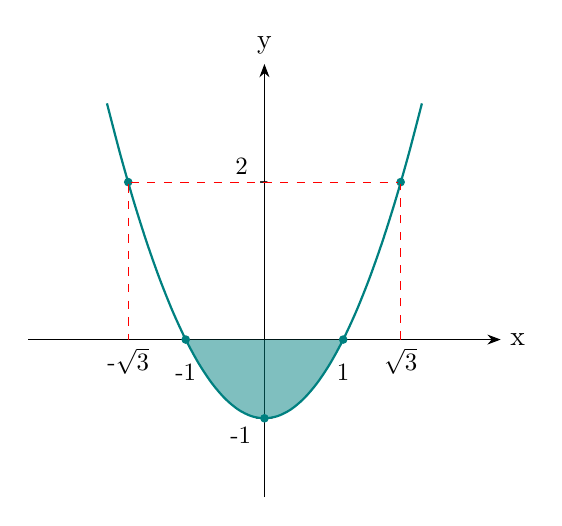
\begin{tikzpicture}[>=stealth]
\draw[-Stealth](-3,0)--(3,0)
node[right]{\text{x}};
\draw[-Stealth](0,-2)--(0,3.5) node[above]{\text{y}};
\draw
(0,2)node[]{-}
(0,-1)node[]{$-$}
(-1,-0.2)node[below,scale=0.9]{-1}
(1,-0.2)node[below,scale=0.9]{1}
(-0.1,2.2)node[left,scale=0.9]{2}
(-0.3,-1)node[below,scale=0.9]{-1}
(1.73,2)node[shape=circle,scale=0.01cm,fill=teal,draw=teal]{}
(-1.73,2)node[shape=circle,scale=0.01cm,fill=teal,draw=teal]{}
(0,-1)node[shape=circle,scale=0.01cm,fill=teal,draw=teal]{}
(-1,0)node[shape=circle,scale=0.01cm,fill=teal,draw=teal]{}
(1,0)node[shape=circle,scale=0.01cm,fill=teal,draw=teal]{};
\draw[scale= 1, domain=-2:2,smooth, variable=\x, teal,thick]plot({\x},{\x*\x-1});
\draw[dashed,color=red!100](1.73,0)--(1.73,1.97)
(-1.73,1.97)--(-1.73,0)
(-1.7,2)--(1.7,2);
\draw(1.73,0)node[below,scale=0.9]{$\sqrt{3}$}
(-1.73,0)node[below,scale=0.9]{-$\sqrt{3}$};
\path[fill=teal,opacity=0.5,domain=-1:1,smooth,variable=\x]plot(\x,\x*\x-1)--(1,0)--(-1,0)--cycle;
\end{tikzpicture}
\end{figure}




















On $[-1,1]$ the smallest value of $x^2-1$ is $-1$, at $x=0$, and the largest is
$0$, at $x=\pm 1$; the function is continuous, so it takes every value in
between. Hence
\begin{align*}
f([-1,1]) &=\{f(x):x\in [-1,1]\}\\
          &=\{x^2-1:x\in [-1,1]\}\\
          &=[-1,0].
\end{align*}
For the inverse image, $x^2-1\in(0,2)$ means $1<x^2<3$, that is
$1<|x|<\sqrt{3}$:
\begin{align*}
f^{-1}\big((0,2)\big) &=\{x:f(x)\in (0,2)\}\\
                      &=\{x:x^2-1\in (0,2)\}\\
                      &=\{x:1<|x|<\sqrt{3}\}\\
                      &=(-\sqrt{3},-1)\cup (1,\sqrt{3}).
\end{align*}
Note that the inverse image is defined for any function; it does not require
$f$ to be invertible, and here $f$ is not.
\end{solution}



\begin{defn}
A function $f:X\longrightarrow Y$ is said to be \emph{injective} (or one-to-one)
if $f(x)=f(y)$ implies that $x=y$. We say that $f$ is \emph{surjective} (or
onto) if $f(X)=Y$, that is, if every element of $Y$ is $f$ of something. A
function which is both injective and surjective is called \emph{bijective}.
\end{defn}

\begin{exa}
The function $f(x)=2x+1$ from $\mathbb{R}$ to $\mathbb{R}$ is bijective.\\\\
\end{exa}


\begin{proof}
Suppose $f(x)=f(y)$. Then $2x+1=2y+1\iff 2x=2y\iff x=y$. Therefore $f$ is injective.
\begin{align*}
\text{Also},\hspace{0.3cm} f(\mathbb{R}) &=\{f(x):x\in \mathbb{R}\}=\{2x+1:x\in \mathbb{R}\}\\
&=\mathbb{R}
\end{align*}
Thus $f$ is surjective. Since $f$ is both injective and surjective, $f$ is
bijective.
\end{proof}





\begin{defn}
Let $X$ be a non-empty set. The function $I:X\longrightarrow X$ defined by $I(x)=x$ is called the identity function on $X$.\\\\
\end{defn}
\begin{defn}
Let $X,Y$ and $Z$ be non-empty sets and $f:X\longrightarrow Y$ and
$g:Y\longrightarrow Z$ be functions. The \emph{composition} of $f$ followed by
$g$ is the function $g\circ f:X\longrightarrow Z$ defined by
$(g\circ f)(x)=g(f(x))$ for all $x\in X$.
\end{defn}
\begin{thm}\label{thm:inverse-exists}
If $f:X\longrightarrow Y$ is a bijective function then there exists a function
$g:Y\longrightarrow X$ such that $g\circ f=I_X$ and $f\circ g=I_Y$.
\end{thm}
\begin{proof}
Since $f$ is surjective, for every $y\in Y$ there is at least one $x\in X$ with
$f(x)=y$; since $f$ is injective there is at most one. So for every $y\in Y$
there is exactly one such $x$, and defining $g(y)$ to be that $x$ assigns to
each $y\in Y$ a unique element of $X$ --- which is what is needed for $g$ to be
a function. Bijectivity is used twice here, once for each half.

To show $g\circ f=I_X$, let $x\in X$ and put $y=f(x)$. Then $g(y)$ is the
unique element mapped by $f$ to $y$, which is $x$, so
$(g\circ f)(x)=g(f(x))=x$. To show $f\circ g=I_Y$, let $y\in Y$. Then
$g(y)$ is the element with $f(g(y))=y$, so $(f\circ g)(y)=y$.
\end{proof}
The function $g$ of Theorem~\ref{thm:inverse-exists} is called the
\emph{inverse function} of $f$, and is written $f^{-1}$.
The next theorem provides some of the properties of images and inverse images of sets under functions.\\\\
\begin{thm}\label{thm:image-props}
Let $f:X\longrightarrow Y$ be a function, $A,B\subset X$ and $C,D\subset Y$.
Then:
\begin{enumerate}
\item $f(A\cup B)=f(A)\cup f(B)$
\item $f(A\cap B)\subset f(A)\cap f(B)$
\item $f^{-1}(C\cup D)=f^{-1}(C)\cup f^{-1}(D)$
\item $f^{-1}(C\cap D)=f^{-1}(C)\cap f^{-1}(D)$
\end{enumerate}
\end{thm}

\begin{proof}
\begin{enumerate}
\item Let $y\in f(A\cup B)$. Then $y=f(x)$ for some $x\in A\cup B$, so $x\in A$
or $x\in B$, whence $y=f(x)\in f(A)$ or $y=f(x)\in f(B)$; that is,
$y\in f(A)\cup f(B)$. Thus $f(A\cup B)\subset f(A)\cup f(B)$.

Conversely, let $y\in f(A)\cup f(B)$, so $y\in f(A)$ or $y\in f(B)$. In the
first case $y=f(x)$ for some $x\in A$, and in the second $y=f(x)$ for some
$x\in B$. Either way $x\in A\cup B$, so $y\in f(A\cup B)$. Hence
$f(A)\cup f(B)\subset f(A\cup B)$, and the two sets are equal.

\item Let $y\in f(A\cap B)$. Then $y=f(x)$ for some $x\in A\cap B$. Since
$x\in A$ we get $y\in f(A)$, and since $x\in B$ we get $y\in f(B)$. Hence
$y\in f(A)\cap f(B)$, which proves $f(A\cap B)\subset f(A)\cap f(B)$.

The reverse inclusion may fail, and it is worth seeing why. If
$y\in f(A)\cap f(B)$ then $y=f(a)$ for some $a\in A$ and $y=f(b)$ for some
$b\in B$ --- but nothing forces $a$ and $b$ to be the \emph{same} point, and
without a common point in $A\cap B$ there is no $x$ to produce $y$ as an image
of the intersection. For a concrete counterexample take
$f:\mathbb{R}\to\mathbb{R}$, $f(x)=x^2$, with $A=\{-1\}$ and $B=\{1\}$. Then
$A\cap B=\emptyset$, so $f(A\cap B)=\emptyset$, while
$f(A)=f(B)=\{1\}$ and therefore $f(A)\cap f(B)=\{1\}$.

If $f$ is injective the difficulty disappears --- $f(a)=f(b)$ then forces
$a=b\in A\cap B$ --- and equality holds.

\item Let $x\in f^{-1}(C\cup D)$. Then $f(x)\in C\cup D$, so $f(x)\in C$ or
$f(x)\in D$, which says $x\in f^{-1}(C)$ or $x\in f^{-1}(D)$; that is,
$x\in f^{-1}(C)\cup f^{-1}(D)$. Hence
$f^{-1}(C\cup D)\subset f^{-1}(C)\cup f^{-1}(D)$.

Conversely, suppose $x\in f^{-1}(C)\cup f^{-1}(D)$, so $x\in f^{-1}(C)$ or
$x\in f^{-1}(D)$, and therefore $f(x)\in C$ or $f(x)\in D$. This means
$f(x)\in C\cup D$, so $x\in f^{-1}(C\cup D)$. Thus
$f^{-1}(C)\cup f^{-1}(D)\subset f^{-1}(C\cup D)$, and the two sets are equal.

\item Here every step is an equivalence, so both inclusions come at once. For
any $x\in X$,
\begin{align*}
x\in f^{-1}(C\cap D) &\iff f(x)\in C\cap D\\
                     &\iff f(x)\in C \ \text{ and }\ f(x)\in D\\
                     &\iff x\in f^{-1}(C) \ \text{ and }\ x\in f^{-1}(D)\\
                     &\iff x\in f^{-1}(C)\cap f^{-1}(D).
\end{align*}
\end{enumerate}
Parts (iii) and (iv) hold for \emph{every} function, with no injectivity
needed, while (ii) is only an inclusion. This asymmetry is worth remembering:
inverse images respect unions and intersections perfectly, images do not.
\end{proof}

\subsection*{Practice Problems}
\addcontentsline{toc}{subsection}{Practice Problems}

\begin{problem}
Let $X=\Big\{\frac{1}{n}:n<5,\ n\in \mathbb{N}\Big\}$ and
$Y=\Big\{\frac{1}{n+2}:n<4,\ n\in \mathbb{N}\Big\}$. List the elements of
$X\cap Y$, $X\cup Y$, $X-Y$, $X\bigtriangledown Y$ and $X\times Y$.
\end{problem}
\begin{solution}
First write out the two sets. Taking $\mathbb{N}=\{1,2,3,\dots\}$, the
condition $n<5$ gives $n=1,2,3,4$, and $n<4$ gives $n=1,2,3$:
$$X=\left\{1,\tfrac{1}{2},\tfrac{1}{3},\tfrac{1}{4}\right\},\qquad
Y=\left\{\tfrac{1}{3},\tfrac{1}{4},\tfrac{1}{5}\right\}.$$
Everything else is read off from these lists.
\begin{align*}
X\cap Y &=\left\{\tfrac{1}{3},\tfrac{1}{4}\right\}\\
X\cup Y &=\left\{1,\tfrac{1}{2},\tfrac{1}{3},\tfrac{1}{4},\tfrac{1}{5}\right\}\\
X-Y &=\left\{1,\tfrac{1}{2}\right\}\\
X\bigtriangledown Y &=(X-Y)\cup(Y-X)
 =\left\{1,\tfrac{1}{2}\right\}\cup\left\{\tfrac{1}{5}\right\}
 =\left\{1,\tfrac{1}{2},\tfrac{1}{5}\right\}
\end{align*}
Finally $X\times Y$ has $4\times 3=12$ ordered pairs:
\begin{align*}
X\times Y=\Big\{&(1,\tfrac13),(1,\tfrac14),(1,\tfrac15),
(\tfrac12,\tfrac13),(\tfrac12,\tfrac14),(\tfrac12,\tfrac15),\\
&(\tfrac13,\tfrac13),(\tfrac13,\tfrac14),(\tfrac13,\tfrac15),
(\tfrac14,\tfrac13),(\tfrac14,\tfrac14),(\tfrac14,\tfrac15)\Big\}.
\end{align*}
Note that $X\times Y$ is a set of \emph{pairs}, not of numbers, and that
$(1,\tfrac13)$ and $(\tfrac13,1)$ are different elements --- the second is not
in $X\times Y$ at all.
\end{solution}

\begin{problem}
If $X$ and $Y$ are any sets, prove that $X-Y=X\cap Y^c$, and deduce that
$X\bigtriangledown Y=(X\cap Y^c)\cup (Y\cap X^c)$.
\end{problem}
\begin{solution}
For the first identity, every step is an equivalence:
\begin{align*}
x\in X-Y &\iff x\in X \ \text{ and }\ x\notin Y\\
         &\iff x\in X \ \text{ and }\ x\in Y^c\\
         &\iff x\in X\cap Y^c.
\end{align*}
Hence $X-Y=X\cap Y^c$.

For the second, apply the first identity twice. By definition
$X\bigtriangledown Y=(X-Y)\cup(Y-X)$, and
$$X-Y=X\cap Y^c,\qquad Y-X=Y\cap X^c,$$
the second by the same argument with $X$ and $Y$ interchanged. Substituting,
$$X\bigtriangledown Y=(X\cap Y^c)\cup (Y\cap X^c).$$
\end{solution}

\begin{problem}
Show that if $X\subset Y$ then $Y^c\subset X^c$.
\end{problem}
\begin{solution}
Let $x\in Y^c$, so $x\notin Y$. Suppose, for contradiction, that $x\in X$.
Since $X\subset Y$, every element of $X$ lies in $Y$, so $x\in Y$ ---
contradicting $x\notin Y$. Therefore $x\notin X$, that is $x\in X^c$.

Since $x$ was an arbitrary element of $Y^c$, we conclude $Y^c\subset X^c$.
Taking complements reverses inclusions; it does not preserve them.
\end{solution}

\begin{problem}
On the set $\mathbb{R}[x]$ of all polynomials with real coefficients, define
$f\mathcal{R}g$ if and only if $f'=g'$. Show that $\mathcal{R}$ is an
equivalence relation and describe its equivalence classes.
\end{problem}
\begin{solution}
All three properties follow from properties of equality of the derivatives.
\begin{enumerate}
\item[i.] \emph{Reflexive.} $f'=f'$, so $f\mathcal{R}f$.
\item[ii.] \emph{Symmetric.} If $f'=g'$ then $g'=f'$, so $f\mathcal{R}g$
implies $g\mathcal{R}f$.
\item[iii.] \emph{Transitive.} If $f'=g'$ and $g'=h'$ then $f'=h'$, so
$f\mathcal{R}g$ and $g\mathcal{R}h$ imply $f\mathcal{R}h$.
\end{enumerate}
For the classes: $f'=g'$ means $(f-g)'=0$, and a polynomial with zero
derivative is constant. So $f\mathcal{R}g$ exactly when $f-g$ is a constant,
and
$$[f]=\{f+c: c\in\mathbb{R}\}.$$
Each class is a family of parallel curves, one for each value of the constant
of integration --- the classes are precisely what is being counted when an
indefinite integral is written with a ``$+\,c$''.
\end{solution}

\begin{problem}
Let $f:\mathbb{R}-\{0\}\rightarrow \mathbb{R}$ be given by $f(x)=\frac{1}{x}$.
Find $f(A)$ where $A=[-1,0)\cup (0,1]$, find $f^{-1}(B)$ where
$B=[-2,-1]\cup [1,2]$, and determine whether $f$ is bijective.
\end{problem}
\begin{solution}
\subhead{The image $f(A)$}
On $(0,1]$, as $x$ decreases from $1$ towards $0$ the value $1/x$ increases
from $1$ without bound, so $f\big((0,1]\big)=[1,\infty)$. On $[-1,0)$ the same
argument with signs reversed gives $f\big([-1,0)\big)=(-\infty,-1]$. Hence
$$f(A)=(-\infty,-1]\cup[1,\infty).$$

\subhead{The inverse image $f^{-1}(B)$}
We need every $x\neq 0$ with $1/x\in[-2,-1]\cup[1,2]$. For $1\leq \frac1x\leq
2$, taking reciprocals reverses the inequalities and gives
$\frac12\leq x\leq 1$. For $-2\leq\frac1x\leq -1$ the same reasoning gives
$-1\leq x\leq -\frac12$. Hence
$$f^{-1}(B)=\left[-1,-\tfrac{1}{2}\right]\cup\left[\tfrac{1}{2},1\right].$$

\subhead{Bijective?}
$f$ is injective: if $\frac1x=\frac1y$ then $x=y$. But $f$ is \emph{not}
surjective onto $\mathbb{R}$, because $\frac1x=0$ has no solution --- $0$ is
not in the range. So $f$ is not bijective as a map into $\mathbb{R}$.

It is worth noticing that this is a defect of the stated codomain only: as a
map $\mathbb{R}-\{0\}\rightarrow\mathbb{R}-\{0\}$ the same rule \emph{is}
bijective, and is its own inverse.
\end{solution}

\begin{problem}
Let $f:X\rightarrow Y$ be a function with $A\subset X$. Decide whether
$f(A^c)=\big(f(A)\big)^c$ is true in general. Give a proof or a counterexample,
and state a condition on $f$ under which it does hold.
\end{problem}
\begin{solution}
The statement is \textbf{false} in general.

\subhead{A counterexample}
Take $f:\mathbb{R}\rightarrow\mathbb{R}$ with $f(x)=x^2$ and $A=[0,\infty)$.
Then $A^c=(-\infty,0)$ and
$$f(A^c)=\{x^2:x<0\}=(0,\infty),$$
while $f(A)=[0,\infty)$ and so $\big(f(A)\big)^c=(-\infty,0)$. These two sets
are not merely unequal --- they are disjoint.

\subhead{Why it fails}
Two separate things go wrong. Because $f$ is not injective, a value can be
reached from both $A$ and $A^c$, so $f(A)$ and $f(A^c)$ may overlap; and
because $f$ is not surjective, a point of $Y$ outside $f(A)$ need not be in
$f(A^c)$ either, since it may not be in the range at all.

\subhead{When it holds}
If $f$ is bijective, both objections vanish and the identity is true. Indeed,
let $y\in Y$ and let $x$ be the unique point with $f(x)=y$. Then
$$y\in f(A^c)\iff x\in A^c \iff x\notin A \iff y\notin f(A)\iff
y\in\big(f(A)\big)^c,$$
where the third equivalence uses injectivity (no \emph{other} point maps to
$y$) and the existence of $x$ uses surjectivity.
\end{solution}

\begin{problem}
Let $f:X\rightarrow Y$ and $g:Y\rightarrow Z$ be functions. Prove that if $f$
and $g$ are both injective then $g\circ f$ is injective, and that if both are
surjective then $g\circ f$ is surjective.
\end{problem}
\begin{solution}
\subhead{Injective}
Suppose $(g\circ f)(x)=(g\circ f)(y)$, that is $g(f(x))=g(f(y))$. Since $g$ is
injective, $f(x)=f(y)$. Since $f$ is injective, $x=y$. Hence $g\circ f$ is
injective. Note the order: $g$'s injectivity is used first, on the outside.

\subhead{Surjective}
Let $z\in Z$. Since $g$ is surjective there is $y\in Y$ with $g(y)=z$. Since
$f$ is surjective there is $x\in X$ with $f(x)=y$. Then
$$(g\circ f)(x)=g(f(x))=g(y)=z,$$
so every $z\in Z$ is attained and $g\circ f$ is surjective.
\end{solution}

\begin{problem}
Let $f:X\rightarrow Y$ and $g:Y\rightarrow Z$ be bijective. Show that
$g\circ f$ is invertible and that $(g\circ f)^{-1}=f^{-1}\circ g^{-1}$.
\end{problem}
\begin{solution}
By the previous problem $g\circ f$ is both injective and surjective, hence
bijective, so by Theorem~\ref{thm:inverse-exists} it has an inverse.

To identify that inverse it is enough to check that $f^{-1}\circ g^{-1}$
composes with $g\circ f$ to give the identity on both sides. Using
associativity of composition and $g^{-1}\circ g=I_Y$,
\begin{align*}
(f^{-1}\circ g^{-1})\circ(g\circ f)
 &=f^{-1}\circ (g^{-1}\circ g)\circ f
 =f^{-1}\circ I_Y\circ f
 =f^{-1}\circ f=I_X,
\end{align*}
and symmetrically
\begin{align*}
(g\circ f)\circ (f^{-1}\circ g^{-1})
 &=g\circ (f\circ f^{-1})\circ g^{-1}
 =g\circ I_Y\circ g^{-1}
 =g\circ g^{-1}=I_Z.
\end{align*}
Hence $(g\circ f)^{-1}=f^{-1}\circ g^{-1}$.

The reversal of order is the point of the result, and it is not a quirk of
notation: to undo ``put on socks, then shoes'' you must take off the shoes
first.
\end{solution}

\pagebreak
\section{MATRICES}
\begin{defn}
Let $m$ and $n$ be positive integers. A rectangular array of the form
$$
\begin{pmatrix}
a_{11}&a_{12}&\cdots&a_{1n}\\
a_{21}&a_{22}&\cdots&a_{2n}\\
\vdots&\vdots&\ddots&\vdots\\
a_{m1}&a_{m2}&\cdots&a_{mn}\\
\end{pmatrix}
$$
is called a \emph{matrix}. It is also written $(a_{ij})_{mn}$, where $i$ indexes
the row and $j$ the column, so $a_{ij}$ is the entry in the $i^{\text{th}}$ row
and $j^{\text{th}}$ column. This matrix has $m$ rows and $n$ columns and is
called an $m$ by $n$ matrix.
\end{defn}

$A=
\begin{pmatrix}
1&2&-3\\0&-1&1\\
\end{pmatrix}
$ is a 2 by 3 matrix. Here the order of the matrix is 2 by 3.\\\\

Two matrices are equal if they have the same order and their corresponding entries are equal for example if $A=
\begin{pmatrix}
a_{11}&a_{12}\\a_{21}&a_{22}\\
\end{pmatrix}
$ and 
$B=
\begin{pmatrix}
b_{11}&b_{12}\\b_{12}&b_{22}
\end{pmatrix}
$ then $A=B$ if and only if $a_{11}=b_{11}$; $a_{12}=b_{12}$, $a_{21}=b_{21}$, $a_{22}=b_{22}$.\\\\






\subsection{Types of Matrices}
Here we will consider some special types of matrices.
\begin{enumerate}
\item The zero matrix is a matrix in which all the entries are zeroes. An example of zero matrix is $
\begin{pmatrix}
0&0&0\\0&0&0\\
\end{pmatrix}
$

\item A matrix in which the number of rows equals the number of columns is called a square matrix
$
\begin{pmatrix}
1&2\\3&4\\
\end{pmatrix}
$ and 
$
\begin{pmatrix}
1&2&1\\4&2&-1\\3&-3&7\\
\end{pmatrix}
$ are squares matrices.

\item A square matrix is called a diagonal matrix if all its non-diagonal entries are zeroes. The matrix 
$
\begin{pmatrix}
1&0&0\\0&2&0\\0&0&3\\
\end{pmatrix}
$ is a diagonal matrix.

\item An identity matrix is a square matrix whose diagonal entries are all ones and the non-diagonal entries are zeroes
$
\begin{pmatrix}
1&0\\ 0&1
\end{pmatrix}
$ and 
$
\begin{pmatrix}
1&0&0\\ 0&1&0\\0&0&1\\
\end{pmatrix}
$ are identity matrices.

\item A square matrix in which all the entries below that leading diagonal are zeroes is called an upper triangular matrix. A lower triangular matrix is a square matrix in which all the elements above the leading diagonal are zeroes 
$
\begin{pmatrix}
6&3&1\\0&2&7\\0&0&1\\
\end{pmatrix}
$ is upper triangular and $
\begin{pmatrix}
4&0&0\\4&2&0\\7&1&-3\\
\end{pmatrix}
$ is lower triangular.

\item The transpose of a matrix $A$, denoted by $A^t$ is the matrix obtained by interchanging the rows and columns of $A$ if $A=
\begin{pmatrix}
1&3&4\\-1&0&2\\
\end{pmatrix}
$, the $ A^t=
\begin{pmatrix}
1&-1\\3&0\\4&2\\
\end{pmatrix}
$

\item A matrix $A$ is said to be symmetric if $A=A^t$. Example $
\begin{pmatrix}
1&0\\0&1\\
\end{pmatrix}^t=
\begin{pmatrix}
1&0\\0&1\\
\end{pmatrix}
$

\item A matrix $A$ is said to be skew-symmetric if $A=-A^t$\\\\
\end{enumerate}







\begin{exa}
The matrix $A=
\begin{pmatrix}
1&-1\\-1&2\\
\end{pmatrix}
$ is symmetric since
$A^t=
\begin{pmatrix}
1&-1\\-1&2\\
\end{pmatrix}
=A$\\\\ 
The matrix $B=
\begin{pmatrix}
0&1\\-1&0\\
\end{pmatrix}
$ is skew-symmetric since $-B^t=
\begin{pmatrix}
0&1\\-1&0\\
\end{pmatrix}
=B$.\\\\
\end{exa}




\subsection{Matrix Algebra}
The sum (difference) of two $m$ by $n$ matrices $A=(a_{ij})$ and $B=(b_{ij})$ is the $m$ by $n$ matrix obtained by adding (subtracting) their corresponding entries.\\ That is $A+B=(a_{ij}+b_{ij})$\\\\
Let $A=
\begin{pmatrix}
1&4\\0&-2\\6&5\\
\end{pmatrix}
$ and 
$B=
\begin{pmatrix}
0&3\\-1&1\\-3&2\\
\end{pmatrix}
$.\\\\\\
Then $A+B=
\begin{pmatrix}
1&7\\-1&-1\\3&7\\
\end{pmatrix}
$ and 
$
A-B=
\begin{pmatrix}
1&1\\1&-3\\9&3\\
\end{pmatrix}
$.\\\\
Let $A=(a_{ij})$ be an $m$ by $n$ matrix and let $c$ be any scalar. Then $cA$ is the matrix obtained by multiplying each entry on $A$ by $c$.\\\\






\begin{exa}
If $A=
\begin{pmatrix}
1&4&6\\2&-1&0\\
\end{pmatrix}
$ and $c=-3$, then $cA=
\begin{pmatrix}
-3&-12&-18\\-6&3&0\\
\end{pmatrix}
$.\\\\
If $A=(a_{ij})$ is an $m$ by $n$ matrix and $B=(b_{ij})$ is an $n$ by $r$ matrix, then the product $C=AB$ is defined at it is an $m$ by $r$ matrix. Then $(i,j)$ entry of the matrix is calculated as follows:\\ $c_{ij}=a_{i1}b_{1j}+a_{i2}b_{2j}+\cdots+a_{in}b_{nj}$.\\\\
\end{exa}



\begin{exa}
$A=
\begin{pmatrix}
-1&-3&3\\1&-1&3\\
\end{pmatrix}
$ and $B=
\begin{pmatrix}
4&0&-3&1\\-5&2&1&-1\\1&-2&0&6\\
\end{pmatrix}
$ then $$AB=
\begin{pmatrix}
-1&-3&3\\1&-1&3\\
\end{pmatrix}
\begin{pmatrix}
4&0&-3&1\\-5&2&1&-1\\1&-2&0&6\\
\end{pmatrix}
=
\begin{pmatrix}
14&-10&0&14\\12&-8&-4&20\\
\end{pmatrix}
$$\\\\
\end{exa}






\begin{exa}
Let $A$ and $B$ be any $m$ by $n$ matrices. Then
\begin{enumerate}
\item $(A+B)^t=A^t+B^t$
\item $(AB)^t=A^tB^t$
\item $(A^t)^t=A$
\item $(A^t)^n=(A^n)^t$ for any positive integer $n$.\\
\end{enumerate}
\end{exa}






\begin{proof}
\begin{enumerate}
\item Let $A=(a_{ij})=A^t$, $B=(b_{ij})=B^t$
\begin{align*}
(A+B) &=(a_{ij}+b_{ij})\\
(A+B)^t &=(a_{ij}+b_{ij})\\
A^t+B^t &=(a_{ij}+b_{ij})\\\\
\therefore \hspace{0.5cm} (A+B)^t &=A^t+B^t\\
\end{align*}

\item
\begin{align*}
(AB)' &=(a_{ij}(b_{ij})=(a_{ij}\hspace{0.1cm}.\hspace{0.1cm}b_{ij})\\\\
(AB)^t &=(a_{ij}\hspace{0.1cm}\cdot\hspace{0.1cm}b_{ij})^t\\
A^t\hspace{0.1cm}\cdot\hspace{0.1cm}B^t &=(a_{ij})^t\hspace{0.1cm}\cdot\hspace{0.1cm}(b_{ij})^t\\
\end{align*}
\end{enumerate}
\end{proof}






\begin{exa}
\begin{enumerate}
\item If $A$ is a square matrix, then $1/2(A+A^t)$ is symmetric and $1/2(A-A^t)$ is skew-symmetric.
\item For any matrix $A$, both $AA^t$ and $A^tA$ are symmetric.\\
\end{enumerate}
\end{exa}


\begin{proof}
\begin{enumerate}
\item
\begin{flushleft}
\begin{align*}
\Big(\frac{1}{2}(A+A^t)\Big)^t &=\frac{1}{2}\Big(A^t+(A^t)^t\Big)\\
&=\frac{1}{2}(A^t+A)\\
&=\frac{1}{2}(A+A^t)\hspace{2cm}\text{and}\\
\end{align*}
\end{flushleft}


\begin{flushright}
\begin{align*}
\Big(\frac{1}{2}(A-A^t)\Big)^t &=\frac{1}{2}\Big(A^t-(A^t)^t\Big)\\
&=\frac{1}{2}(A^t-A)\\
&=-\frac{1}{2}(A-A^t)\\
\end{align*}
\end{flushright}

\item
$(AA^t)^t =(A^t)^tA^t =AA^t\hspace{0.4cm}
 \text{and}\hspace{0.4cm} (A^tA)^t = A^t(A^t)^t=A^tA$\\\\
\end{enumerate}
\end{proof}





\subsection{Non-Singular Matrices}

\begin{defn}
An $n$ by $m$ matrix is said to be non-singular if there exists a matrix $B$,denoted by $A^{-1}$, such that $AB=BA=I_n$ where $I_n$ is the $n$ by $n$ identity matrix.\\
Non-singular matrices are also called invertible matrices. A matrix which is not non-singular is called singular.\\\\
\end{defn}



\begin{exa}
The matrix $A=
\begin{pmatrix}
-2&5\\1&-3\\
\end{pmatrix}
$ is non-singular if $B=
\begin{pmatrix}
-3&-5\\-1&-2\\
\end{pmatrix}
$ then $AB=
\begin{pmatrix}
1&0\\0&1\\
\end{pmatrix}
$ and $BA=
\begin{pmatrix}
1&0\\0&1\\
\end{pmatrix}
$.\\\\\\
\end{exa}




\begin{thm}
If $A$ is a non-singular matrix, then its inverse is unique.\\\\
\end{thm}

\begin{proof}
Suppose $B$ and $C$ are both inverses of $A$. Then $AB=BA=I$ and $AC=CA=I$.\\ Therefore, $B=B\cdot I=B(AC)=(BA)C=I\cdot C=C$. Thus $B=C$.\\\\
\end{proof}
The next theorem gives properties of non-singular matrices.\\\\


\begin{thm}
Let $A$ and $B$ be non-singular $n$ by $n$ matrices and $k$ be a non-zero real number. Then
\begin{enumerate}
\item $A^{-1}$ is non-singular and $(A^{-1})^{-1}=A$.
\item $kA$ is non-singular and $(kA)^{-1}=\dfrac{1}{k}\,A^{-1}$.
\item $AB$ is non-singular and $(AB)^{-1}=A^{-1}B^{-1}$.
\item $A^t$ is non-singular and $(A^t)^{-1}=(A^{-1})^t$.\\
\end{enumerate}
\end{thm}




\begin{proof}
\begin{enumerate}
\item Since $A^{-1}A=AA^{-1}=I$, $A^{-1}$ is non-singular and $(A^{-1})^{-1}=A$.
\item We have $(kA)\Big(\dfrac{1}{k}\,A^{-1}\Big)=k\cdot\dfrac{1}{k}\,A\cdot A^{-1}=I$ and $\Big(\dfrac{1}{k}\,A^{-1}\Big)(kA)=\dfrac{1}{k}\cdot kA^{-1}A=I$.\\\\
\end{enumerate}
\end{proof}


\subsection{Elementary Row Operations On Matrices}

The following are called elementary row operations on a matrix.
\begin{enumerate}
\item Interchange the $i^{\text{th}}$ and $j^{\text{th}}$ rows; $r_i\longleftrightarrow r_j$. For instance$$
\begin{pmatrix}
1&2\\3&4\\
\end{pmatrix}
\hspace{0.5cm} 
\begin{matrix}
r_1 \longleftrightarrow r_2\\ \longrightarrow\\
\end{matrix}
\hspace{0.5cm}
\begin{pmatrix}
3&4\\1&2\\
\end{pmatrix}
$$
\item Multiply the $i^{\text{th}}$ row by $\alpha$, where $\alpha$ is a non-zero scalar; $r_i\longrightarrow \alpha r_j$. For example
$$
\begin{pmatrix}
1&2\\3&4\\
\end{pmatrix}
\hspace{0.5cm}
\begin{matrix}
r_1\longrightarrow 2r_1\\
\end{matrix}
\hspace{0.5cm}
\begin{pmatrix}
2&4\\3&4\\
\end{pmatrix}
$$
\item Add the $i^{\text{th}}$ row to $\alpha$ times the $j^{\text{th}}$ row; $r_i\longrightarrow r_i+\alpha r_j$. For example
$$
\begin{pmatrix}
1&2\\3&4\\
\end{pmatrix}
\hspace{0.5cm}
\begin{matrix}
r_1\longrightarrow r_1+2r_2\\
\end{matrix}
\hspace{0.5cm}
\begin{pmatrix}
7&10\\3&4\\
\end{pmatrix}
$$
\end{enumerate}



\begin{defn}
Two $m$ by $n$ matrices $A$ and $B$ are said to be row equivalent if $B$ can be obtained from $A$ by a finite sequence of elementary row operations.\\\\
\end{defn}
\begin{exa}
$
\begin{pmatrix}
1&-3&1&0\\-1&2&4&1\\1&0&-2&1\\
\end{pmatrix}
$ is row equivalent to $
\begin{pmatrix}
1&-3&1&0\\0&-1&5&1\\0&1&1&1\\
\end{pmatrix}
$ since
\begin{align*}
\begin{pmatrix}
1&-3&1&0\\-1&2&4&1\\1&0&-2&1\\
\end{pmatrix}
&\hspace{0.5cm}
\begin{matrix}
r_3\longrightarrow r_3+r_2\\
\end{matrix}
\hspace{0.5cm}
\begin{pmatrix}
1&-3&1&0\\-1&2&4&1\\0&2&2&2\\
\end{pmatrix}\\\\
&\hspace{0.5cm}
\begin{matrix}
r_2\longrightarrow r_2+r_1\\ r_3\longrightarrow \frac{1}{2}r_3\\
\end{matrix}
\hspace{0.5cm}
\begin{pmatrix}
1&-3&1&0\\0&-1&5&1\\0&1&1&1\\
\end{pmatrix}
\end{align*}
\end{exa}



\begin{defn}
An $m$ by $n$ matrix $A$ is called an echelon matrix if it satisfies the following:
\begin{enumerate}
\item[i.] the leading non-zero element in every row is 1.
\item[ii.] the leading 1 in each row occurs to the right of the leading 1 in any preceding row.
\item[iii.] non-zero rows appear before zero rows.\\
\end{enumerate}
\end{defn}



\begin{defn}
A reduced echelon matrix is an echelon matrix with the property that the leading 1 in every row is the only non-zero element in the column in which it occurs.\\\\
\end{defn}
\begin{exa}
$
\begin{pmatrix}
1&0&3&4\\0&1&-1&0\\0&0&1&5\\
\end{pmatrix}
$ is an echelon matrix but not a reduced echelon matrix.\\\\\\
$
\begin{pmatrix}
1&0&0&0\\0&1&0&0\\0&0&1&0\\0&0&0&1
\end{pmatrix}
$ is a reduced echelon matrix.\\\\\\
\end{exa}


\begin{exa}
Find the reduced echelon of\hspace{0.5cm} (a) $
\begin{pmatrix}
1&1&0\\1&-3&0\\
\end{pmatrix}
\hspace{0.5cm}$ (b) 
$
\begin{pmatrix}
3&1&-2\\-4&2&1\\-1&0&1\\
\end{pmatrix}
$.\\\\
\end{exa}
\begin{solution}
\begin{align*}
\text{(a)}\hspace{0.4cm}
\begin{pmatrix}
1&1&0\\1&-3&0\\
\end{pmatrix}
&
\hspace{0.3cm}
\begin{matrix}
r_2\longrightarrow r_2-r_1\\
\end{matrix}
\hspace{0.3cm}
\begin{pmatrix}
1&1&0\\0&-4&0\\
\end{pmatrix}
\hspace{0.3cm}
\begin{matrix}
r_2\longrightarrow-\frac{1}{2}r_2\\
\end{matrix}
\hspace{0.3cm}
\begin{pmatrix}
1&1&0\\0&1&0\\
\end{pmatrix}\\\\
&\hspace{0.3cm}
\begin{matrix}
r_1\longrightarrow r_1-r_2\\
\end{matrix}
\hspace{0.3cm}
\begin{pmatrix}
1&0&0\\0&1&0\\
\end{pmatrix}\\
\end{align*}

\begin{align*}
\text{(b)}\hspace{0.4cm}
\begin{pmatrix}
3&1&-2\\ -4&2&1\\-1&0&1\\
\end{pmatrix}
&\hspace{0.3cm}
\begin{matrix}
r_1\rightarrow r_1+3r_2\\ \longrightarrow\\ r_2\rightarrow r_2-4r_3\\
\end{matrix}
\hspace{0.3cm}
\begin{pmatrix}
0&1&1\\0&2&-3\\-1&0&1\\
\end{pmatrix}
\hspace{0.3cm}
\begin{matrix}
r_1\leftrightarrow r_3\\ \longrightarrow\\
\end{matrix}
\begin{pmatrix}
-1&0&1\\0&2&-3\\0&1&1\\
\end{pmatrix}\\\\
&\hspace{0.3cm}
\begin{matrix}
r_2\rightarrow r_2-2r_3\\ \longrightarrow\\
\end{matrix}
\hspace{0.3cm}
\begin{pmatrix}
-1&0&1\\0&0&-5\\0&1&1\\
\end{pmatrix}
\hspace{0.3cm}
\begin{matrix}
r_2\leftrightarrow r_3\\ \longrightarrow\\ r_1\rightarrow -r_1\\
\end{matrix}
\hspace{0.3cm}
\begin{pmatrix}
1&0&-1\\0&1&1\\0&0&-5\\
\end{pmatrix}\\\\
&\hspace{0.3cm}
\begin{matrix}
r_3\rightarrow -\frac{1}{5}r_3\\
\end{matrix}
\hspace{0.3cm}
\begin{pmatrix}
1&0&-1\\0&1&1\\0&0&1\\
\end{pmatrix}
\hspace{0.3cm}
\begin{matrix}
r_1\rightarrow r_1+r_3\\ \longrightarrow\\ r_2\rightarrow r_2-r_3\\
\end{matrix}
\hspace{0.3cm}
\begin{pmatrix}
1&0&0\\ 0&1&0\\0&0&1\\
\end{pmatrix}\\
\end{align*}




\pagebreak
\end{solution}


\subsection{Elementary Matrices}

\begin{defn}
An elementary matrix is a matrix obtained by applying an elementary row operation to the identity matrix.\\\\
\end{defn}

\begin{exa}
The matrices 
$
\begin{pmatrix}
-1&0\\0&1\\
\end{pmatrix}
\hspace{0.4cm}
\begin{pmatrix}
1&0\\0&-1\\
\end{pmatrix}
$ and $
\begin{pmatrix}
1&2\\0&1\\
\end{pmatrix}
$ are elementary matrices. The corresponding elementary row operations are $r_1\longrightarrow -r_1,\hspace{0.3cm} r_2\longrightarrow -r_2,\hspace{0.3cm}r_1\longrightarrow r_1-2r_2$.\\\\
\end{exa}
The following theorem provides some of the properties of elementary matrices.\\

\begin{thm}\label{thm:elementary-matrices}
\begin{enumerate}
\item If a matrix $B$ can be obtained from a matrix $A$ by applying an
elementary row operation, then $B=EA$, where $E$ is the elementary matrix
corresponding to that operation.
\item Every elementary matrix is non-singular, and the inverse of an elementary
matrix is again elementary.
\item If $B$ can be obtained from $A$ by a finite sequence of elementary row
operations, then there are elementary matrices $E_1,E_2,\dots,E_k$ such that
$B=E_kE_{k-1}\cdots E_1A$.
\item If $R$ is the reduced echelon matrix of $A$, then there are elementary
matrices $E_1,E_2,\dots,E_k$ such that $A=E_1E_2\cdots E_kR$.
\end{enumerate}
\end{thm}

\begin{proof}
\begin{enumerate}
\item Write $e$ for the row operation and $E=e(I)$ for the elementary matrix it
produces. The key observation is that row $i$ of a product $MA$ depends only on
row $i$ of $M$: explicitly, $(MA)_{i\bullet}=\sum_{j}m_{ij}A_{j\bullet}$, a
combination of the rows of $A$ with the coefficients taken from row $i$ of $M$.

Now each of the three elementary operations changes the rows of $I$ in a
particular way, and applying $E$ to $A$ reproduces exactly that change on the
rows of $A$. For instance, if $e$ is $r_i\rightarrow r_i+kr_j$, then row $i$ of
$E$ is $\text{(row $i$ of $I$)}+k\,\text{(row $j$ of $I$)}$, so row $i$ of $EA$
is $A_{i\bullet}+kA_{j\bullet}$, while every other row of $E$ is a row of $I$
and leaves the corresponding row of $A$ unchanged. That is precisely $e(A)$.
The other two operations are checked the same way. Hence $B=e(A)=EA$.

\item Every elementary row operation can be undone by an elementary row
operation of the same type:
$$r_i\leftrightarrow r_j \ \text{ by }\ r_i\leftrightarrow r_j,\qquad
r_i\rightarrow kr_i \ \text{ by }\ r_i\rightarrow \tfrac{1}{k}r_i \ (k\neq 0),
\qquad
r_i\rightarrow r_i+kr_j \ \text{ by }\ r_i\rightarrow r_i-kr_j.$$
Let $e'$ be the operation undoing $e$, and $E'=e'(I)$ the corresponding
elementary matrix. Applying part (1) twice, $E'E=e'(E)=e'(e(I))=I$ and
similarly $EE'=I$. So $E$ is invertible with $E^{-1}=E'$, which is elementary.

\item Induction on the number of operations. If $B$ is obtained from $A$ by
operations $e_1,\dots,e_k$ applied in that order, let $A_0=A$ and
$A_t=e_t(A_{t-1})$, so $B=A_k$. By part (1), $A_t=E_tA_{t-1}$ for each $t$.
Composing,
$$B=A_k=E_kA_{k-1}=E_kE_{k-1}A_{k-2}=\cdots=E_kE_{k-1}\cdots E_1A.$$

\item By definition $R$ is obtained from $A$ by a finite sequence of elementary
row operations, so part (3) gives $R=E_kE_{k-1}\cdots E_1A$. By part (2) each
$E_t$ is invertible, so we may multiply on the left successively by
$E_k^{-1},E_{k-1}^{-1},\dots$ to obtain
$$A=E_1^{-1}E_2^{-1}\cdots E_k^{-1}R,$$
and each $E_t^{-1}$ is elementary, again by part (2). Renaming these inverses
$E_1,\dots,E_k$ gives the statement.
\end{enumerate}
\end{proof}

\begin{remark}
Part (1) is the reason elementary row operations can be treated as
\emph{multiplication by a matrix} rather than as an informal procedure. It is
what makes the rest of the subject possible: once row reduction is matrix
multiplication, facts about it can be proved rather than merely described.

Note the order in part (3): the operation applied \emph{first} contributes the
matrix nearest to $A$, so the elementary matrices appear in reverse order of
application.
\end{remark}
\begin{exa}
Find $A^{-1}$ for $A=
\begin{pmatrix}
-1&1&2\\ 1&1&0\\ 0&-2&-1\\
\end{pmatrix}
$
\end{exa}


\begin{solution}
\begin{align*}
& \begin{pmatrix}
-1&1&2&&|&1&0&0\\ 1&1&0&&|&0&1&0\\0&-2&-1&&|&0&0&1\\
\end{pmatrix}
\hspace{0.3cm}
\begin{matrix}
r_2\rightarrow r_2+r_1\\ \longrightarrow\\ r_3\rightarrow -r_3\\
\end{matrix}
\hspace{0.3cm}
\begin{pmatrix}
-1&1&2&&|&1&0&0\\0&2&2&&|&1&1&0\\0&2&1&&|&0&0&-1\\
\end{pmatrix}\\\\
&\hspace{0.3cm}
\begin{matrix}
r_3\rightarrow r_3-r_2\\ \longrightarrow\\
\end{matrix}
\hspace{0.3cm}
\begin{pmatrix}
-1&1&2&&|&1&0&0\\0&2&2&&|&1&1&0\\0&0&-1&&|&-1&-1&-1\\
\end{pmatrix}
\hspace{0.3cm}
\begin{matrix}
r_2\rightarrow \frac{1}{2}r_2\\ \longrightarrow\\ r_3\rightarrow -r_3\\
\end{matrix}
\hspace{0.3cm}
\begin{pmatrix}
-1&1&2&&|&1&0&0\\0&1&1&&|&1/2&1/2&0\\0&0&1&&|&1&1&1\\
\end{pmatrix}\\\\
&\hspace{0.3cm}
\begin{matrix}
r_2\rightarrow r_2-r_3\\ \longrightarrow\\
\end{matrix}
\hspace{0.3cm}
\begin{pmatrix}
-1&1&2&&|&1&0&0\\0&1&0&&|&-1/2&-1/2&-1\\0&0&1&&|&1&1&1\\
\end{pmatrix}\\\\
\hspace{0.3cm}&
\begin{matrix}
r_1\rightarrow -r_1\\ \longrightarrow\\
\end{matrix}
\hspace{0.3cm}
\begin{pmatrix}
1&-1&-2&&|&-1&0&0\\0&1&0&&|&-1/2&-1/2&-1\\0&0&1&&|&1&1&1\\
\end{pmatrix}\\\\
&\hspace{0.3cm}
\begin{matrix}
r_1\rightarrow r_1+r_2\\ \longrightarrow\\
\end{matrix}
\hspace{0.3cm}
\begin{pmatrix}
1&0&-2&&|&-3/2&-1/2&-1\\0&1&0&&|&-1/2&-1/2&-1\\0&0&1&&|&1&1&1\\
\end{pmatrix}\\\\
&\hspace{0.3cm}
\begin{matrix}
r_1\rightarrow r_1+2r_3\\ \longrightarrow\\
\end{matrix}
\hspace{0.3cm}
\begin{pmatrix}
1&0&0&&|&1/2&3/2&1\\0&1&0&&|&-1/2&-1/2&-1\\0&0&1&&|&1&1&1\\
\end{pmatrix}\\
\end{align*}


$$\therefore\hspace{0.3cm}
A^{-1}=
\begin{pmatrix}
1/2&3/2&1\\-1/2&-1/2&-1\\1&1&1\\
\end{pmatrix}
$$\\


\pagebreak
\end{solution}

\subsection{Normal Form of a Matrix}
Elementary column operations are defined similarly to elementary row operations.\\

\begin{defn}
By a finite sequence of elementary row/column operations: an $m$ by $n$ matrix $A$ can be reduced to one of the forms $$I_r,\hspace{0.3cm}
\begin{bmatrix}
I_r\\0\\
\end{bmatrix}
,\hspace{0.3cm}
\begin{bmatrix}
I_r&0\\
\end{bmatrix}
\hspace{0.3cm}\text{or}\hspace{0.3cm}
\begin{bmatrix}
I_r&0\\0&0\\
\end{bmatrix}
$$ called the normal form of $A$. $I_r$ is an $r$ by $r$ identity matrix where $1\leq r\leq m$ and $1\leq r\leq n$, and $0$ represents a block of zeroes.\\\\
\end{defn}
\begin{exa}
Find the normal form of the matrix
$
\begin{pmatrix}
-1&0&2\\1&-2&3\\2&0&4\\
\end{pmatrix}
$.\\\\
\end{exa}
\begin{solution}
\begin{align*}
\begin{pmatrix}
-1&0&2\\1&-2&3\\2&0&4\\
\end{pmatrix}
&\hspace{0.3cm}
\begin{matrix}
r_2\rightarrow r_2+r_1\\ \longrightarrow\\ r_3\rightarrow r_3+2r_1\\
\end{matrix}
\hspace{0.3cm}
\begin{pmatrix}
-1&0&2\\0&-2&5\\0&0&8\\
\end{pmatrix}
\hspace{0.3cm}
\begin{matrix}
r_3\rightarrow \frac{1}{8}r_3\\ \longrightarrow\\
\end{matrix}
\hspace{0.3cm}
\begin{pmatrix}
-1&0&2\\0&-2&5\\0&0&1\\
\end{pmatrix}\\\\
&\hspace{0.3cm}
\begin{matrix}
r_2\rightarrow r_2-5r_3\\ \longrightarrow\\ r_1\rightarrow r_1-2r_3\\
\end{matrix}
\hspace{0.3cm}
\begin{pmatrix}
-1&0&0\\0&-2&0\\0&0&1\\
\end{pmatrix}
\hspace{0.3cm}
\begin{matrix}
r_1\rightarrow -r_1\\ \longrightarrow\\ r_2\rightarrow -\frac{1}{2}r_2\\
\end{matrix}
\hspace{0.3cm}
\begin{pmatrix}
1&0&0\\0&1&0\\0&0&1\\
\end{pmatrix}\\
\end{align*}
Therefore the normal form of $
\begin{pmatrix}
-1&0&2\\1&-2&3\\2&0&4\\
\end{pmatrix}
$ is $I_3$.\\\\\\
\end{solution}



\begin{exa}
Find the normal form of the matrix $A=
\begin{pmatrix}
0&5&13&6\\-4&2&3&1\\0&0&3&-1\\0&-2&-3&6.\\
\end{pmatrix}
$.\\\\
\end{exa}



\begin{solution}
$$
\begin{pmatrix}
0&5&13&6\\-4&2&3&1\\0&0&3&-1\\0&-2&-3&6\\
\end{pmatrix}
\hspace{0.3cm}
\begin{matrix}
r_1\leftrightarrow r_2\\ \longrightarrow\\ r_3\leftrightarrow r_4\\
\end{matrix}
\hspace{0.3cm}
\begin{pmatrix}
-4&2&3&1\\0&5&13&6\\0&-2&-3&6\\0&0&3&-1\\
\end{pmatrix}
\hspace{0.3cm}
\begin{matrix}
r_2\rightarrow r_2+2r_3\\ \longrightarrow\\
\end{matrix}
\hspace{0.3cm}
\begin{pmatrix}
-4&2&3&1\\0&1&7&18\\0&-2&-3&6\\0&0&3&-1\\
\end{pmatrix}
$$
\begin{align*}
&
\begin{matrix}
r_3\rightarrow r_3+2r_2\\ \longrightarrow\\
\end{matrix}
\hspace{0.3cm}
\begin{pmatrix}
-4&2&3&1\\0&1&7&18\\0&0&11&42\\0&0&3&-1\\
\end{pmatrix}
\hspace{0.3cm}
\begin{matrix}
c_1\rightarrow -\frac{1}{4}c_1\\ \longrightarrow\\
\end{matrix}
\hspace{0.3cm}
\begin{pmatrix}
1&2&3&1\\0&1&7&18\\0&0&11&42\\0&0&3&-1\\
\end{pmatrix}
\hspace{0.3cm}
\begin{matrix}
c_2\rightarrow c_2-2c_1\\c_3\rightarrow c_3-3c_1\\ \longrightarrow\\ c_4\rightarrow c_4-c_1\\
\end{matrix}\\\\
&
\begin{pmatrix}
1&0&0&0\\0&1&7&18\\0&0&11&42\\0&0&3&-1\\
\end{pmatrix}
\hspace{0.3cm}
\begin{matrix}
c_3\rightarrow c_3-7c_2\\ \longrightarrow\\ c_4\rightarrow c_4-18c_2\\
\end{matrix}
\hspace{0.3cm}
\begin{pmatrix}
1&0&0&0\\0&1&0&0\\0&0&11&42\\0&0&3&-1\\
\end{pmatrix}
\hspace{0.3cm}
\begin{matrix}
c_4\rightarrow c_4-4c_3\\ \longrightarrow\\
\end{matrix}
\hspace{0.3cm}
\begin{pmatrix}
1&0&0&0\\0&1&0&0\\0&0&11&-2\\0&0&3&-13\\
\end{pmatrix}\\\\
&
\begin{matrix}
r_4\rightarrow r_4-3/11r_3\\ \longrightarrow\\
\end{matrix}
\hspace{0.3cm}
\begin{pmatrix}
1&0&0&0\\0&1&0&0\\0&0&11&-2\\0&0&0&-137/11\\
\end{pmatrix}
\hspace{0.3cm}
\begin{matrix}
r_4\rightarrow -\frac{11}{137}r_4\\ \longrightarrow\\
\end{matrix}
\hspace{0.3cm}
\begin{pmatrix}
1&0&0&0\\0&1&0&0\\0&0&11&-2\\0&0&0&1\\
\end{pmatrix}
\hspace{0.3cm}
\begin{matrix}
r_3\rightarrow r_3+2r_4\\ \longrightarrow\\
\end{matrix}\\\\
&
\begin{pmatrix}
1&0&0&0\\0&1&0&0\\0&0&11&0\\0&0&0&1\\
\end{pmatrix}
\hspace{0.3cm}
\begin{matrix}
r_3\rightarrow \frac{1}{11}\\ \longrightarrow\\
\end{matrix}
\hspace{0.3cm}
\begin{pmatrix}
1&0&0&0\\0&1&0&0\\0&0&1&0\\0&0&0&1\\
\end{pmatrix}
\hspace{0.3cm} = I_4\\
\end{align*}
\end{solution}




\begin{defn}
Two matrices $A$ and $B$ are said to be equivalent if there exist invertible matrices $P$ and $Q$ such that $PAQ=B$.\\\\
\end{defn}
The next theorem shows that every matrix is equivalent to its normal form.\\\\
\begin{thm}\label{thm:normal-form}
If $A$ is an $m$ by $n$ matrix, then there exist an invertible $m$ by $m$ matrix
$P$ and an invertible $n$ by $n$ matrix $Q$ such that $PAQ=N$, where $N$ is the
normal form of $A$. In particular every matrix is equivalent to its normal
form.
\end{thm}

\begin{proof}
By definition of the normal form, $A$ can be carried to $N$ by a finite
sequence of elementary row operations followed by a finite sequence of
elementary column operations.

By Theorem~\ref{thm:elementary-matrices}(1), performing the row operations is
the same as multiplying on the left by elementary $m$ by $m$ matrices
$E_1,\dots,E_k$, in the order applied. The corresponding statement for columns
is proved in the same way, with the roles of rows and columns exchanged:
applying an elementary column operation to $A$ is multiplication on the
\emph{right} by the $n$ by $n$ elementary matrix obtained by applying that
operation to $I_n$. Let $F_1,\dots,F_l$ be those matrices. Then
$$E_k\cdots E_1\,A\,F_1\cdots F_l=N.$$
Put $P=E_k\cdots E_1$ and $Q=F_1\cdots F_l$, so that $PAQ=N$. Each $E_t$ and
each $F_t$ is invertible by Theorem~\ref{thm:elementary-matrices}(2), and a
product of invertible matrices is invertible, so $P$ and $Q$ are invertible ---
of sizes $m$ by $m$ and $n$ by $n$ respectively, as required.
\end{proof}

\begin{remark}
The proof also says how to \emph{find} $P$ and $Q$, which is what the next
example does: carry out the reduction while performing the same row operations
on an adjoined copy of $I_m$ and the same column operations on an adjoined copy
of $I_n$. Whatever those copies become is $P$ and $Q$.
\end{remark}



\begin{exa}
Find invertible matrices $P$ and $Q$ such that $PAQ=N$, where $A=
\begin{pmatrix}
-1&0&2\\1&-2&3\\
\end{pmatrix}
$ and $N$ is the normal form of $A$.\\\\
\end{exa}



\begin{solution}
\begin{align*}
&
\begin{pmatrix}
-1&0&2&&|&1&0\\1&-2&3&&|&0&1\\
\end{pmatrix}
\hspace{0.3cm}
\begin{matrix}
r_2\rightarrow r_2+r_1\\ \longrightarrow\\
\end{matrix}
\hspace{0.3cm}
\begin{pmatrix}
-1&0&2&&|&1&0\\0&-2&5&&|&1&1\\
\end{pmatrix}
\hspace{0.3cm}
\begin{matrix}
r_1\rightarrow -r_1\\ \longrightarrow\\
\end{matrix}\\\\
&
\begin{pmatrix}
1&0&-2&&|&-1&0\\0&-2&5&&|&1&1\\
\end{pmatrix}
\hspace{0.3cm}
\begin{matrix}
r_2\rightarrow -\frac{1}{2}r_2\\ \longrightarrow\\
\end{matrix}
\hspace{0.3cm}
\begin{pmatrix}
1&0&-2&&|&-1&0\\0&1&-5/2&&|&-1/2&-1/2\\
\end{pmatrix}\\
\end{align*}

Take $P=
\begin{pmatrix}
-1&0\\\\-1/2&-1/2\\
\end{pmatrix}
$\\
\begin{align*}
&\text{Now}\hspace{0.3cm}
\begin{pmatrix}
1&0&-2&&|&1&0&0\\0&1&-5/2&&|&0&1&0\\&&&&|&0&0&1\\
\end{pmatrix}
\hspace{0.3cm}
\begin{matrix}
c_3\rightarrow c_3+2c_1\\ \longrightarrow\\
\end{matrix}
\hspace{0.3cm}
\begin{pmatrix}
1&0&0&&|&1&0&2\\0&1&-5/2&&|&0&1&0\\&&&&|&0&0&1\\
\end{pmatrix}\\\\
&
\begin{matrix}
c_3\rightarrow c_3+2c_2\\ \longrightarrow\\
\end{matrix}
\hspace{0.3cm}
\begin{pmatrix}
1&0&0&&|&1&0&2\\0&1&0&&|&0&1&5/2\\&&&&|&0&0&1\\
\end{pmatrix}\\
\end{align*}
$$\text{Take}\hspace{0.4cm}Q=
\begin{pmatrix}
1&0&2\\0&1&5/2\\0&0&1\\
\end{pmatrix}
$$\\

$$\text{Then}\hspace{0.3cm} PAQ=
\begin{pmatrix}
-1&0\\-1/2&-1/2\\
\end{pmatrix}
\begin{pmatrix}
-1&0&2\\1&-2&3\\
\end{pmatrix}
\begin{pmatrix}
1&0&2\\0&1&5/2\\0&0&1\\
\end{pmatrix}
=
\begin{pmatrix}
1&0&0\\0&1&0\\
\end{pmatrix}
$$



\end{solution}

\subsection*{Practice Problems}
\addcontentsline{toc}{subsection}{Practice Problems}

\begin{problem}
Let $A=\begin{pmatrix}-1&2\\0&1\end{pmatrix}$ and
$B=\begin{pmatrix}1&1\\-1&0\end{pmatrix}$. Find $A^3$ and
$A^2+2AB+B^2-A^{-1}B^{-1}+3I$.
\end{problem}
\begin{solution}
Compute $A^2$ first, because it makes everything else shorter:
$$A^2=\begin{pmatrix}-1&2\\0&1\end{pmatrix}
      \begin{pmatrix}-1&2\\0&1\end{pmatrix}
     =\begin{pmatrix}1&0\\0&1\end{pmatrix}=I.$$
So $A$ is its own inverse, and therefore
$$A^3=A^2A=IA=A=\begin{pmatrix}-1&2\\0&1\end{pmatrix},\qquad A^{-1}=A.$$
For the second expression, the pieces are
$$AB=\begin{pmatrix}-3&-1\\-1&0\end{pmatrix},\qquad
B^2=\begin{pmatrix}0&1\\-1&-1\end{pmatrix},\qquad
B^{-1}=\begin{pmatrix}0&-1\\1&1\end{pmatrix},$$
the last because $\det B=1$. Then
$A^{-1}B^{-1}=AB^{-1}=\begin{pmatrix}2&3\\1&1\end{pmatrix}$, and adding
everything up,
\begin{align*}
A^2+2AB+B^2-A^{-1}B^{-1}+3I
&=\begin{pmatrix}1&0\\0&1\end{pmatrix}
 +\begin{pmatrix}-6&-2\\-2&0\end{pmatrix}
 +\begin{pmatrix}0&1\\-1&-1\end{pmatrix}
 -\begin{pmatrix}2&3\\1&1\end{pmatrix}
 +\begin{pmatrix}3&0\\0&3\end{pmatrix}\\
&=\begin{pmatrix}-4&-4\\-4&2\end{pmatrix}.
\end{align*}
Note that $2AB$ is genuinely needed here: $A$ and $B$ do not commute, so
$(A+B)^2$ is \emph{not} $A^2+2AB+B^2$ and the expression cannot be shortened
that way.
\end{solution}

\begin{problem}
Let $A=\begin{pmatrix}1&0&-1\\2&-1&0\\0&0&1\end{pmatrix}$. Verify that $AA^t$
and $A^tA$ are symmetric, that $\frac{1}{2}(A+A^t)$ is symmetric and that
$\frac{1}{2}(A-A^t)$ is skew-symmetric. Explain why the first two facts hold
for \emph{every} matrix.
\end{problem}
\begin{solution}
The computations give
$$AA^t=\begin{pmatrix}2&2&-1\\2&5&0\\-1&0&1\end{pmatrix},\qquad
  A^tA=\begin{pmatrix}5&-2&-1\\-2&1&0\\-1&0&2\end{pmatrix},$$
and both are visibly equal to their own transposes. Also
$$\tfrac{1}{2}(A+A^t)=\begin{pmatrix}1&1&-1/2\\1&-1&0\\-1/2&0&1\end{pmatrix},
\qquad
  \tfrac{1}{2}(A-A^t)=\begin{pmatrix}0&-1&-1/2\\1&0&0\\1/2&0&0\end{pmatrix},$$
the first symmetric, the second skew-symmetric (note its diagonal is zero, as
it must be: $s_{ii}=-s_{ii}$ forces $s_{ii}=0$).

None of this depends on the particular $A$. Using $(XY)^t=Y^tX^t$ and
$(X^t)^t=X$,
$$(AA^t)^t=(A^t)^tA^t=AA^t,$$
so $AA^t$ is symmetric for every $A$, and the same argument applies to $A^tA$.
Likewise
$$\left(\tfrac{1}{2}(A+A^t)\right)^t=\tfrac{1}{2}(A^t+A)=\tfrac{1}{2}(A+A^t),
\qquad
\left(\tfrac{1}{2}(A-A^t)\right)^t=\tfrac{1}{2}(A^t-A)=-\tfrac{1}{2}(A-A^t).$$
Adding the last two gives $A$ itself, so \emph{every} square matrix splits as a
symmetric part plus a skew-symmetric part, and that splitting is unique.
\end{solution}

\begin{problem}
Find the reduced echelon matrix of
$A=\begin{pmatrix}3&-1&2\\-5&7&3\end{pmatrix}$.
\end{problem}
\begin{solution}
Make the leading entry $1$, clear the column below it, then clear upwards.
\begin{align*}
\begin{pmatrix}3&-1&2\\-5&7&3\end{pmatrix}
&\xrightarrow{\ r_1\rightarrow \frac{1}{3}r_1\ }
\begin{pmatrix}1&-1/3&2/3\\-5&7&3\end{pmatrix}
\xrightarrow{\ r_2\rightarrow r_2+5r_1\ }
\begin{pmatrix}1&-1/3&2/3\\0&16/3&19/3\end{pmatrix}\\[2mm]
&\xrightarrow{\ r_2\rightarrow \frac{3}{16}r_2\ }
\begin{pmatrix}1&-1/3&2/3\\0&1&19/16\end{pmatrix}
\xrightarrow{\ r_1\rightarrow r_1+\frac{1}{3}r_2\ }
\begin{pmatrix}1&0&17/16\\0&1&19/16\end{pmatrix}.
\end{align*}
So the reduced echelon matrix is
$\begin{pmatrix}1&0&17/16\\0&1&19/16\end{pmatrix}$, and $A$ has rank $2$.
\end{solution}

\begin{problem}
Use elementary row operations to find the inverse of
$A=\begin{pmatrix}-1&2&3\\1&0&-1\\2&1&-3\end{pmatrix}$.
\end{problem}
\begin{solution}
Adjoin $I$ and reduce the left half to $I$; whatever the right half becomes is
$A^{-1}$. Carrying this out gives
$$A^{-1}=\begin{pmatrix}1/4&9/4&-1/2\\1/4&-3/4&1/2\\1/4&5/4&-1/2\end{pmatrix}.$$
It is worth checking the answer rather than trusting the arithmetic:
$$AA^{-1}=\begin{pmatrix}-1&2&3\\1&0&-1\\2&1&-3\end{pmatrix}
\begin{pmatrix}1/4&9/4&-1/2\\1/4&-3/4&1/2\\1/4&5/4&-1/2\end{pmatrix}
=\begin{pmatrix}1&0&0\\0&1&0\\0&0&1\end{pmatrix}.$$
For instance the $(1,1)$ entry is
$(-1)\frac14+2\cdot\frac14+3\cdot\frac14=\frac{-1+2+3}{4}=1$, and the $(1,2)$
entry is $(-1)\frac94+2\left(-\frac34\right)+3\cdot\frac54
=\frac{-9-6+15}{4}=0$.
\end{solution}

\begin{problem}
Express $A=\begin{pmatrix}1&0&-1\\2&1&2\\-3&2&-3\end{pmatrix}$ in the form
$E_1E_2\cdots E_kR$, where the $E_i$ are elementary matrices and $R$ is the
reduced echelon form of $A$. What is $R$ here, and why?
\end{problem}
\begin{solution}
Row reducing $A$ gives $R=I_3$: the matrix has rank $3$. This is forced, not a
coincidence --- a square reduced echelon matrix of full rank has a leading $1$
in every row and zeros elsewhere in those columns, and the only such matrix is
the identity.

The reduction can be done with the six operations
$$r_2\rightarrow r_2-2r_1,\quad r_3\rightarrow r_3+3r_1,\quad
r_3\rightarrow r_3-2r_2,\quad r_3\rightarrow -\tfrac{1}{14}r_3,\quad
r_1\rightarrow r_1+r_3,\quad r_2\rightarrow r_2-4r_3.$$
The fourth is easy to forget: after the third operation the last row is
$(0,0,-14)$, and it must be scaled to a leading $1$ before it can be used to
clear the column above it.

With $E'_t$ the elementary matrix of the $t$-th operation,
$E'_6E'_5\cdots E'_1A=I$. By Theorem~\ref{thm:elementary-matrices}(2) each
$E'_t$ is invertible with elementary inverse, so multiplying back through,
$$A=(E'_1)^{-1}(E'_2)^{-1}\cdots (E'_6)^{-1}R,$$
which is the required form with $E_t=(E'_t)^{-1}$. Concretely
$$(E'_1)^{-1}=\begin{pmatrix}1&0&0\\2&1&0\\0&0&1\end{pmatrix},\qquad
  (E'_2)^{-1}=\begin{pmatrix}1&0&0\\0&1&0\\-3&0&1\end{pmatrix},\qquad
  (E'_4)^{-1}=\begin{pmatrix}1&0&0\\0&1&0\\0&0&-14\end{pmatrix}.$$
An inverse of an ``add a multiple'' operation is the identity with the sign of
the multiplier flipped; the inverse of a scaling is the reciprocal scaling.

Since $R=I$ here, the factorisation also says $A$ is a product of elementary
matrices, which is true of every invertible matrix.
\end{solution}

\begin{problem}
Find invertible matrices $P$ and $Q$ such that $PAQ=N$ is the normal form of
$A=\begin{pmatrix}1&-1\\2&0\\-3&2\end{pmatrix}$.
\end{problem}
\begin{solution}
$A$ is $3$ by $2$, so $P$ is $3$ by $3$ and $Q$ is $2$ by $2$. Row reduce,
recording the operations on a copy of $I_3$:
$$r_2\rightarrow r_2-2r_1,\qquad r_3\rightarrow r_3+3r_1,\qquad
r_2\rightarrow \tfrac{1}{2}r_2,\qquad r_3\rightarrow r_3+r_2,\qquad
r_1\rightarrow r_1+r_2,$$
which carries $A$ to $\begin{pmatrix}1&0\\0&1\\0&0\end{pmatrix}$. That is
already the normal form $N=\begin{pmatrix}I_2\\0\end{pmatrix}$, so no column
operations are needed and $Q=I_2$. Applying the same operations to $I_3$ gives
$$P=\begin{pmatrix}0&1/2&0\\-1&1/2&0\\2&1/2&1\end{pmatrix},\qquad Q=I_2,
\qquad PAQ=\begin{pmatrix}1&0\\0&1\\0&0\end{pmatrix}.$$
The rank of $A$ is $2$, which is what the number of leading ones in $N$ records
--- and by Theorem~\ref{thm:normal-form} that number is the same whatever
sequence of operations is used.
\end{solution}

\begin{problem}
Prove that if $A$ is invertible then its inverse is unique, and that
$(AB)^{-1}=B^{-1}A^{-1}$ whenever $A$ and $B$ are both invertible.
\end{problem}
\begin{solution}
\subhead{Uniqueness}
Suppose $B$ and $C$ both satisfy $AB=BA=I$ and $AC=CA=I$. Then
$$B=BI=B(AC)=(BA)C=IC=C,$$
so there is only one such matrix. The argument uses only associativity and the
two-sided identity property; note that it needs $B$ to be a \emph{left} inverse
and $C$ a \emph{right} inverse, which is why both equations are assumed.

\subhead{The inverse of a product}
It suffices to check that $B^{-1}A^{-1}$ works, since by the first part nothing
else can:
$$(AB)(B^{-1}A^{-1})=A(BB^{-1})A^{-1}=AIA^{-1}=AA^{-1}=I,$$
$$(B^{-1}A^{-1})(AB)=B^{-1}(A^{-1}A)B=B^{-1}IB=B^{-1}B=I.$$
Hence $AB$ is invertible with $(AB)^{-1}=B^{-1}A^{-1}$. The order reverses, for
the same reason it reverses for the inverse of a composition of functions.
\end{solution}

\begin{problem}
Let $A$ be an $n$ by $n$ matrix. Show that $A$ is invertible if and only if its
reduced echelon form is $I_n$.
\end{problem}
\begin{solution}
Let $R$ be the reduced echelon form of $A$. By
Theorem~\ref{thm:elementary-matrices}(3) there are elementary matrices with
$R=E_k\cdots E_1A$, and by part (2) of the same theorem each is invertible, so
$R=PA$ with $P=E_k\cdots E_1$ invertible.

If $R=I_n$ then $PA=I$, and since $P$ is invertible, $A=P^{-1}$, which is
invertible.

Conversely suppose $A$ is invertible. Then $R=PA$ is a product of invertible
matrices and so is invertible. Now $R$ is a square reduced echelon matrix; if
it had a row of zeros it would send some non-zero vector to $0$ and could not
be invertible, so every row of $R$ contains a leading $1$. With $n$ leading
ones in $n$ columns, and zeros above and below each, $R=I_n$.
\end{solution}

\pagebreak
\section{SYSTEMS OF LINEAR EQUATIONS}



\subsection{Substitution and Gaussian Elimination}
To solve a system of linear equations by substitution, we start by making one variable the subject of the formula in one of the equations. Then we substitute for this variable in one of the remaining equations. We keep substituting until the fewest number of variables possible remain. The solution can then be obtained.\\

\begin{exa}
Use the substitution method to solve the system of linear equations.
\begin{align*}
-x+y+z &=1\\x-y+z &=2\\x+y-z &=3\\
\end{align*}
\end{exa}


\begin{solution}
From the first equation, $x=y+z-1$ substitute for $x$ in the second equation. $y+z-1-y+z=2$ or $2z=3$; Thus $z=3/2$. From the third equation, we obtain $x=-y+9/2$ and from $x=y+z-1$, we have $x=y+1/2$. Thus $x=5/2$ and $y=2$.\\\\


\end{solution}
The next example illustrates the Gaussian elimination method for solving systems of linear equations.\\\\
\begin{exa}
Use the method of Gaussian elimination to solve the system of linear equations.
\begin{align*}
x-2y+z &-1\\3x+y-4z&=3\\-2x+4y+3z&=-2\\
\end{align*}
\end{exa}


\begin{solution}
Multiply the first equation by 2 and add to the third equation $5z=-4$ of $z=-4/5$. Therefore the system reduces to
\begin{align*}
z&=-4/5\\
3x+y-4z&=3\\-2x+4y+3z &=-2
\end{align*}
Multiply the second equation by 2 and the third equation by 3 then add
\begin{align*}
z&=-4/5\\14y+z&=0\\ -2x+4y+3z&=2\\\\ \implies\hspace{0.4cm}(x,y,z)&=\Big(\frac{7}{2},\frac{3}{70},\frac{-4}{5}\Big)\\
\end{align*}
\end{solution}


\subsection{Elementary Row Operations and Systems of Linear Equations}
The substitution and Gaussian elimination methods for solving systems of linear equations work well for systems with a small number of variables. For systems with many equations and many variables, these methods become innefficient. In this section the Gaussian elimination method will be developed to a more efficient method for solving systems of linear equations with many variables or many equations.\\\\


\begin{defn}
The augmented matrix of the system of linear equations
\begin{align*}
a_{11}x_1+a_{12}x_2+\cdots+a_{1n}x_n &=b_1\\
a_{21}x_1+a_{22}x_2+\cdots+a_{2n}x_n &=b_2\\
\vdots\\
a_{n1}x_1+a_{n2}x_2+\cdots+a_{mn}x_n&=b_m\\
\end{align*}
is the matrix
$
\begin{pmatrix}
a_{11}&a_{12}&\cdots&a_{1n}&&|&b_1\\
a_{21}&a_{22}&\cdots&a_{2n}&&|&b_2\\
.&&&.&&|&.\\
.&&&.&&|&.\\
.&&&.&&|&.\\
a_{m1}&a_{m2}&\cdots&a_{mn}&&|&b_{mn}\\
\end{pmatrix}
=\Big(A/b\Big)$ where $A$ is the coefficient matrix\\\\
$
A=
\begin{pmatrix}
a_{11}&a_{12}&\cdots&a_{1n}\\
a_{21}&a_{22}&\cdots&a_{2n}\\
\vdots&\vdots&\ddots&\vdots\\
a_{m1}&a_{m2}&\cdots&a_{mn}\\
\end{pmatrix}
\hspace{0.3cm}$
and 
$\hspace{0.3cm}
b=
\begin{pmatrix}
b_1\\b_2\\.\\.\\.\\b_m\\
\end{pmatrix}
$\\\\\\
\end{defn}

\begin{exa}
The system of linear equations.
\begin{align*}
x+2y+3z&=4\\2x+3y+4z&=5\\3x+4y+5y&=6\\
\end{align*}
has coefficient matrix
$
\begin{pmatrix}
1&2&3\\2&3&4\\3&4&5\\
\end{pmatrix}
$
and augmented matrix
$
\begin{pmatrix}
1&2&3&&|&4\\2&3&4&&|&5\\3&4&5&&|&6\\
\end{pmatrix}
$\\\\\\\\




The following terminology is used for systems of linear equations
\begin{enumerate}
\item An $n$-tuple $(x_1,x_2,\dots,x_n)$ which satisfies each of the $m$
equations in the system $$\sum^n_{j=1}a_{ij}x_j=b_i\qquad(i=1,2,\dots,m)$$ is
called a solution of the system.
\item Two systems of linear equations are equivalent if every solution of one
system is a solution of the other and vice versa --- that is, if they have the
same solution set.
\item A system with at least one solution is called consistent. An inconsistent
system is one with no solution.
\end{enumerate}
\end{exa}

\begin{thm}\label{thm:row-ops-systems}
\begin{enumerate}
\item If $(A'|b')=(a'_{ij}|b'_i)$ is the $m$ by $n+1$ matrix obtained from
$(A|b)$ by a single elementary row operation, then the systems
$$\sum^n_{j=1}a'_{ij}x_j=b'_i \qquad\text{and}\qquad \sum^n_{j=1}a_{ij}x_j=b_i
\qquad(i=1,2,\dots,m)$$
are equivalent.
\item If $(R|s)$ is the reduced echelon matrix of the augmented matrix $(A|b)$,
then the systems $\sum^n_{j=1}r_{ij}x_j=s_i$ and $\sum^n_{j=1}a_{ij}x_j=b_i$
$(i=1,\dots,m)$ are equivalent.
\item A system of linear equations is consistent if and only if the reduced
echelon matrix of its augmented matrix has no leading element in its last
column.
\end{enumerate}
\end{thm}

\begin{proof}
\begin{enumerate}
\item Read each row of the augmented matrix as an equation. The three
elementary row operations then say, respectively: list two of the equations in
the other order; multiply one equation through by a non-zero constant $k$; add
$k$ times one equation to another.

None of these changes the solution set. If $(x_1,\dots,x_n)$ satisfies all the
original equations then it satisfies each of the new ones, since each new
equation is a consequence of the old ones. Conversely --- and this is the part
that needs the restriction $k\neq 0$ --- each operation can be undone by an
operation of the same kind (Theorem~\ref{thm:elementary-matrices}(2)), so by
the same argument every solution of the new system is a solution of the old.
Hence the two solution sets contain each other and the systems are equivalent.

\item $(R|s)$ is obtained from $(A|b)$ by a finite sequence of elementary row
operations. Applying part (1) once for each operation, the solution set is
unchanged at every step, so the first and last systems are equivalent.

\item Suppose the reduced echelon matrix has a leading element in its last
column. That leading element is a $1$ in some row $i$, and being a leading
element it is the first non-zero entry of its row, so every $r_{ij}$ is zero.
Row $i$ therefore reads
$$0\cdot x_1+0\cdot x_2+\cdots+0\cdot x_n=1,$$
which no $n$-tuple satisfies. By part (2) the original system has the same
solution set, so it too is inconsistent.

Conversely, suppose there is no leading element in the last column. Then every
leading element sits in one of the first $n$ columns. Call the variables
belonging to those columns \emph{leading} and the rest \emph{free}. Assign the
value $0$ to every free variable; each equation containing a leading element
then determines its leading variable outright, and any row with no leading
element is the equation $0=0$, which is satisfied. This produces a solution, so
the system is consistent.
\end{enumerate}
\end{proof}

\begin{remark}
Part (3) is what makes row reduction a decision procedure rather than merely a
simplification: after reducing, consistency can be read off by looking at one
column, and the proof of the converse also shows how to write down a solution
when one exists.
\end{remark}


\begin{exa}
Solve the system
\begin{align*}
3x-y+4z&=-2\\-x+y+2z&=1\\6x+3y-z&=4
\end{align*}
\end{exa}
\begin{solution}
\begin{align*}
&
\begin{pmatrix}
3&-1&4&|&-2\\-1&1&2&|&1\\6&3&-1&|&4\\
\end{pmatrix}
\hspace{0.3cm}
\begin{matrix}
r_1\rightarrow r_1+3r_2\\ \longrightarrow\\ r_3\rightarrow r_3+6r_2\\
\end{matrix}
\hspace{0.3cm}
\begin{pmatrix}
0&2&10&|&1\\-1&1&2&|&1\\0&9&11&|&10\\
\end{pmatrix}
\hspace{0.3cm}
\begin{matrix}
r_1\leftrightarrow r_2\\ \longrightarrow\\
\end{matrix}\\\\
&
\begin{pmatrix}
-1&1&2&|&1\\0&2&10&|&1\\0&9&11&|&10\\
\end{pmatrix}
\hspace{0.3cm}
\begin{matrix}
r_3\rightarrow r_3-r_2\\ \longrightarrow\\
\end{matrix}
\hspace{0.3cm}
\begin{pmatrix}
-1&1&2&|&1\\0&2&10&|&1\\0&7&1&|&9\\
\end{pmatrix}
\hspace{0.3cm}
\begin{matrix}
r_2\rightarrow \frac{1}{2}r_2\\ \longrightarrow\\
\end{matrix}
\hspace{0.3cm}
\begin{pmatrix}
-1&1&2&|&1\\0&1&5&|&1/2\\0&7&1&|&9\\
\end{pmatrix}\\\\
&
\begin{matrix}
r_3\rightarrow r_3-7r_2\\ \longrightarrow\\
\end{matrix}
\hspace{0.3cm}
\begin{pmatrix}
-1&1&2&|&1\\0&1&5&|&1/2\\0&0&-34&|&11/2\\
\end{pmatrix}
\hspace{0.3cm}
\begin{matrix}
r_1\rightarrow r_1-r_2\\ \longrightarrow\\ r_3\rightarrow -\frac{1}{34}r_3\\
\end{matrix}
\hspace{0.3cm}
\begin{pmatrix}
-1&0&-3&|&1/2\\0&1&5&|&1/2\\0&0&1&|&-11/68\\
\end{pmatrix}\\
\end{align*}
$$
\begin{matrix}
r_1\rightarrow r_1+3r_3\\ \longrightarrow\\ r_2\rightarrow r_2-5r_3\\
\end{matrix}
\hspace{0.4cm}
\begin{pmatrix}
-1&0&0&|&1/68\\0&1&0&|&-21/68\\0&0&1&|&-11/68
\end{pmatrix}
$$\\
$$\text{Therefore,}\hspace{0.4cm}(x,y,z)=\Big(\frac{1}{68},-\frac{21}{68},-\frac{11}{68}\Big)\hspace{0.4cm}\text{is the solution.}$$\\
\end{solution}
For some systems of linear equations there is a parameter whose value determines the nature of the solution of the system. This is illustrated in the following example.\\\\


\begin{exa}
Find the value of $t$ for which the system
\begin{align*}
x+y+tz&=1\\x+ty+z&=1\\tx+y+z&=-2
\end{align*}
has (i). no solution  (ii). a unique solution (iii). infinitely many solutions.\\\\
\end{exa}


\begin{solution}
\begin{align*}
&
\begin{pmatrix}
1&1&t&|&1\\1&t&1&|&1\\t&1&1&|&-2\\
\end{pmatrix}
\hspace{0.3cm}
\begin{matrix}
r_1\leftrightarrow r_3\\ \longrightarrow\\
\end{matrix}
\hspace{0.3cm}
\begin{pmatrix}
t&1&1&|&-2\\1&t&1&|&1\\1&1&t&|&1\\
\end{pmatrix}
\hspace{0.3cm}
\begin{matrix}
r_3\rightarrow r_3-r_1\\ \longrightarrow\\
\end{matrix}
\hspace{0.3cm}
\begin{pmatrix}
t&1&1&|&-2\\1&t&1&|&1\\1-t&0&t-1&|&3\\
\end{pmatrix}\\\\
&
\begin{matrix}
r_2\rightarrow r_2-r_1\\ \longrightarrow\\
\end{matrix}
\hspace{0.3cm}
\begin{pmatrix}
t&1&1&|&-2\\1-t&t-1&0&|&3\\1-t&0&t-1&|&3\\
\end{pmatrix}
\hspace{0.3cm}
\begin{matrix}
r_2\rightarrow \frac{1}{1-t}r_2\\ \longrightarrow\\ r_3\rightarrow \frac{1}{1-t}r_3\\
\end{matrix}
\hspace{0.3cm}
\begin{pmatrix}
t&1&1&|&-2\\1&-1&0&|&3/1-t\\1&0&-1&|&3/1-t\\
\end{pmatrix}\\\\
&
\begin{matrix}
r_3\rightarrow r_3-r_2\\ \longrightarrow\\
\end{matrix}
\hspace{0.3cm}
\begin{pmatrix}
t&1&1&|&-2\\1&-1&0&|&3/1-t\\0&1&-1&|&0\\
\end{pmatrix}
\hspace{0.3cm}
\begin{matrix}
r_1\rightarrow r_1+r_3\\ \longrightarrow\\
\end{matrix}
\hspace{0.3cm}
\begin{pmatrix}
t&2&0&|&-2\\1&-1&0&|&3/1-t\\0&1&-1&|&0\\
\end{pmatrix}\\\\
&
\begin{matrix}
r_1\rightarrow r_1+2r_2\\ \longrightarrow\\
\end{matrix}
\hspace{0.3cm}
\begin{pmatrix}
t+2&0&0&|&\frac{2t+4}{1-t}\\\\ 1&-1&0&|&\frac{3}{1-t}\\\\0&1&-1&|&0\\
\end{pmatrix}
\hspace{0.3cm}
\begin{matrix}
r_1\rightarrow (1/t+2)r_2\\ \longrightarrow\\
\end{matrix}
\hspace{0.3cm}
\begin{pmatrix}
1&0&0&|&\frac{2t+4}{(t+2)(1-t)}\\\\1&-1&0&|&\frac{3}{1-t}\\\\ 0&1&-1&|&0\\
\end{pmatrix}\\\\
&
\begin{matrix}
r_2\rightarrow r_2-r_1\\ \longrightarrow\\
\end{matrix}
\hspace{0.3cm}
\begin{pmatrix}
1&0&0&|&\frac{2}{(1-t)}\\0&-1&0&|&\frac{1}{1-t}\\0&1&-1&|&0\\
\end{pmatrix}
\hspace{0.3cm}
\begin{matrix}
r_3\rightarrow r_3+r_2\\ \longrightarrow\\
\end{matrix}
\hspace{0.3cm}
\begin{pmatrix}
1&0&0&|&\frac{2}{1-t}\\0&-1&0&|&\frac{1}{1-t}\\0&0&-1&|&\frac{1}{1-t}\\
\end{pmatrix}\\\\
&
\begin{matrix}
r_1\rightarrow (1-t)r_1\\ \longrightarrow\\ r_2\rightarrow (1-t)r_2\\ r_3\rightarrow (1-t)r_3\\
\end{matrix}
\hspace{0.3cm}
\begin{pmatrix}
1-t&0&0&|&2\\0&1-t&0&|&1\\0&0&t-1&|&1\\
\end{pmatrix}
\end{align*}

(i). $t-1=0,\hspace{0.4cm} t=1\hspace{1cm}$ (ii). $t\neq 0\hspace{1cm}$ (iii). No values of $t$ satisfy this requirement.\\



\pagebreak
\end{solution}

\subsection{Homogeneous Systems of Linear Equations}
\begin{defn}
A homogeneous system of linear equations is a system of the form;
\begin{align*}
a_{11}x_1+a_{12}x_2+\cdots+a_{1n}x_n &=0\\
a_{21}x_1+a_{22}x_2+\cdots+a_{2n}x_n &=0\\
\vdots\\
a_{m1}x_1+a_{m2}x_2+\cdots+a_{mn}x_n &=0
\end{align*}
In shortened notation, this is denoted by $\sum\limits^n_{j=1}a_{ij}x_j=0$ $(i=1,2,\dots, m)$\\\\
The $n$-tuple $(0,0,0,\dots,0)$ is always a solution of the homogeneous system. It is called the trivial solution of the system.\\
\end{defn}

\begin{exa}
The system of linear equations
\begin{align*}
x+y+z &=0\\
2x-3y-z&=0\\
4x+5y+2z &=0
\end{align*}
is a homogeneous system.\\
\end{exa}

\begin{thm}\label{thm:homogeneous}
\begin{enumerate}
\item If the number of equations is less than the number of variables in a
homogeneous system of linear equations, then the system has a non-trivial
solution.
\item A system of $n$ homogeneous linear equations in $n$ variables has a
non-trivial solution if and only if $R\neq I_n$, where $R$ is the reduced
echelon matrix of the coefficient matrix of the system.
\end{enumerate}
\end{thm}

\begin{proof}
Both parts turn on counting leading elements. Reduce the augmented matrix
$(A|0)$ to reduced echelon form. Row operations combine rows, so a column of
zeros stays a column of zeros: the augmented column remains $0$ throughout, and
the reduced augmented matrix is $(R|0)$ where $R$ is the reduced echelon matrix
of $A$. In particular there is never a leading element in the last column,
which by Theorem~\ref{thm:row-ops-systems}(3) confirms what we already knew ---
a homogeneous system is always consistent, the trivial solution being one.

Let $r$ be the number of leading elements of $R$. Each occupies its own row and
its own column, so the $n$ variables split into $r$ leading variables and
$n-r$ free ones, and by
Theorem~\ref{thm:row-ops-systems}(2) the original system is equivalent to the
reduced one. Assigning arbitrary values to the free variables determines the
leading variables uniquely, so:
$$\text{the system has a non-trivial solution}\iff n-r>0 \iff r<n,$$
since if $n-r>0$ we may set one free variable to $1$ and obtain a solution
which is not all zeros, while if $r=n$ every variable is leading and the
reduced equations read $x_1=0,\dots,x_n=0$.

\begin{enumerate}
\item Each leading element lies in its own row, so $r\leq m$, the number of
equations. If $m<n$ then $r\leq m<n$, so $r<n$ and a non-trivial solution
exists.

\item Here $R$ is $n$ by $n$. If $R=I_n$ then $r=n$ and only the trivial
solution exists. If $R\neq I_n$ then $r<n$ --- a square reduced echelon matrix
with a leading element in every row is the identity --- so a non-trivial
solution exists.
\end{enumerate}
\end{proof}

\begin{remark}
Part (1) is the formal version of a fact worth carrying: \emph{more unknowns
than equations always leaves room to move.} It is the same statement as
Theorem~\ref{thm:rank-nullity}(ii), seen from the matrix side rather than the
linear-map side.
\end{remark}

\begin{exa}
Find the values of $t$ for which the homogeneous system
\begin{align*}
x+5y+3z &=0\\5x+y-z &=0\\x+2y+tz &=0
\end{align*}
has a non-trivial solution.\\
\end{exa}

\begin{solution}
\begin{align*}
\begin{pmatrix}
1&5&3&|&0\\5&1&-1&|&0\\1&2&t&|&0\\
\end{pmatrix}
& \hspace{0.3cm}
\begin{matrix}
r_2\rightarrow r_2-5r_1\\ \longrightarrow\\ r_3\rightarrow r_3-r_1\\
\end{matrix}
\hspace{0.3cm}
\begin{pmatrix}
1&5&3&|&0\\0&-24&-16&|&0\\ 0&-3&t-3&|&0\\
\end{pmatrix}
\hspace{0.3cm}
\begin{matrix}
r_2\rightarrow -\frac{1}{8}r_2\\ \longrightarrow\\ r_3\rightarrow -r_3\\
\end{matrix}\\\\
&
\hspace{0.3cm}
\begin{pmatrix}
1&5&3&|&0\\ 0&3&2&|&0\\0&3&-t+3&|&0\\
\end{pmatrix}
\hspace{0.3cm}
\begin{matrix}
r_3\rightarrow r_3-r_2\\ \longrightarrow\\
\end{matrix}
\hspace{0.3cm}
\begin{pmatrix}
1&5&3&|&0\\ 0&3&2&|&0\\0&0&-t+1&|&0\\
\end{pmatrix}
\end{align*}
$\therefore$ The system has a non-trivial solution when $t=1$.
\end{solution}

\subsection*{Practice Problems}
\addcontentsline{toc}{subsection}{Practice Problems}

\begin{problem}
Solve the system
$$\frac{1}{x}+\frac{2}{y}-\frac{4}{z}=1,\qquad
  \frac{2}{x}+\frac{3}{y}+\frac{8}{z}=0,\qquad
 -\frac{1}{x}+\frac{9}{y}+\frac{10}{z}=5.$$
\end{problem}
\begin{solution}
The system is not linear in $x,y,z$, but it is linear in the reciprocals. Put
$$u=\frac1x,\qquad v=\frac1y,\qquad w=\frac1z,$$
which is legitimate because none of $x,y,z$ may be zero for the equations to
make sense. The system becomes
$$u+2v-4w=1,\qquad 2u+3v+8w=0,\qquad -u+9v+10w=5,$$
and row reducing the augmented matrix gives
$$u=-\frac{7}{13},\qquad v=\frac{54}{91},\qquad w=-\frac{8}{91}.$$
Inverting,
$$x=-\frac{13}{7},\qquad y=\frac{91}{54},\qquad z=-\frac{91}{8}.$$
Substituting back into the first equation as a check:
$-\frac{7}{13}+2\cdot\frac{54}{91}-4\cdot\left(-\frac{8}{91}\right)
=-\frac{49}{91}+\frac{108}{91}+\frac{32}{91}=\frac{91}{91}=1.$

The lesson is that a substitution can make a non-linear system linear; what
must be checked is that the substitution is reversible on the domain in
question, which here means $x,y,z\neq 0$.
\end{solution}

\begin{problem}
Solve the system
$$x_1+x_2+x_3=a,\qquad 2x_1+2x_3=b,\qquad 3x_2+3x_3=c,$$
where $a,b,c$ are constants. For which $a,b,c$ is it consistent?
\end{problem}
\begin{solution}
Divide the second equation by $2$ and the third by $3$:
$$x_1+x_2+x_3=a,\qquad x_1+x_3=\tfrac{b}{2},\qquad x_2+x_3=\tfrac{c}{3}.$$
Subtracting the second from the first gives $x_2=a-\frac{b}{2}$. Substituting
into the third gives
$$x_3=\frac{c}{3}-x_2=\frac{c}{3}-a+\frac{b}{2},$$
and then the second equation gives
$$x_1=\frac{b}{2}-x_3=\frac{b}{2}-\frac{c}{3}+a-\frac{b}{2}=a-\frac{c}{3}.$$
So the solution is
$$x_1=a-\frac{c}{3},\qquad x_2=a-\frac{b}{2},\qquad
  x_3=\frac{b}{2}+\frac{c}{3}-a,$$
and it exists and is unique for \emph{every} $a,b,c$: the coefficient matrix
has rank $3$, so by Theorem~\ref{thm:row-ops-systems} there is never a leading
element in the augmented column. A square system with an invertible coefficient
matrix is consistent whatever the right-hand side.
\end{solution}

\begin{problem}
For what values of $a$ does the system
$$x+2y-3z=4,\qquad 3x-y+5z=2,\qquad 4x+y+(a^2-14)z=a+2$$
have (i) no solution, (ii) a unique solution, (iii) infinitely many solutions?
\end{problem}
\begin{solution}
Row reduce the augmented matrix, using the first row to clear the first column:
$$\begin{pmatrix}1&2&-3&|&4\\3&-1&5&|&2\\4&1&a^2-14&|&a+2\end{pmatrix}
\xrightarrow[\ r_3\rightarrow r_3-4r_1\ ]{\ r_2\rightarrow r_2-3r_1\ }
\begin{pmatrix}1&2&-3&|&4\\0&-7&14&|&-10\\0&-7&a^2-2&|&a-14\end{pmatrix}.$$
Now $r_3\rightarrow r_3-r_2$ gives
$$\begin{pmatrix}1&2&-3&|&4\\0&-7&14&|&-10\\0&0&a^2-16&|&a-4\end{pmatrix}.$$
Everything is decided by the last row, whose coefficient is
$a^2-16=(a-4)(a+4)$.
\begin{enumerate}
\item[(ii)] If $a\neq 4$ and $a\neq -4$ the coefficient is non-zero, the third
variable is determined, and there is a \textbf{unique solution}.
\item[(iii)] If $a=4$ the last row is $0=0$, which imposes no condition. There
are two leading elements and three variables, so one free variable remains and
there are \textbf{infinitely many solutions}.
\item[(i)] If $a=-4$ the last row reads $0=-8$, which is impossible, so there
is \textbf{no solution}.
\end{enumerate}
Note that $a=4$ and $a=-4$ both make the determinant vanish, but they behave
differently. A zero determinant tells you the solution is not unique; it does
not tell you which of the other two cases you are in --- for that the augmented
column must be looked at.
\end{solution}

\begin{problem}
Determine conditions on $\lambda$ and $\mu$ so that
$$2x+3y+z=5,\qquad 3x-y+\lambda z=2,\qquad x+7y-6z=\mu$$
has (i) a unique solution, (ii) no solution, (iii) infinitely many solutions.
\end{problem}
\begin{solution}
The determinant of the coefficient matrix is
$$\det\begin{pmatrix}2&3&1\\3&-1&\lambda\\1&7&-6\end{pmatrix}=-11(\lambda-8).$$
\begin{enumerate}
\item[(i)] If $\lambda\neq 8$ the determinant is non-zero, the coefficient
matrix is invertible, and there is a \textbf{unique solution} for every $\mu$.
\item[] For $\lambda=8$ the determinant vanishes and $\mu$ decides. Eliminate
$x$ using the third equation:
$$r_1-2r_3:\ -11y+13z=5-2\mu,\qquad r_2-3r_3:\ -22y+26z=2-3\mu.$$
The left-hand side of the second is exactly twice that of the first, so the two
are consistent only if $2-3\mu=2(5-2\mu)$, that is $\mu=8$.
\item[(iii)] If $\lambda=8$ and $\mu=8$ the second equation is a consequence of
the first, leaving two independent equations in three unknowns:
\textbf{infinitely many solutions}.
\item[(ii)] If $\lambda=8$ and $\mu\neq 8$ the two equations contradict each
other: \textbf{no solution}.
\end{enumerate}
\end{solution}

\begin{problem}
Consider $ax+by=0$, $cx+dy=0$, $ex+fy=0$ as three lines in the plane. Describe
their relative positions when the system has (i) only the trivial solution,
(ii) non-trivial solutions.
\end{problem}
\begin{solution}
Every one of these lines passes through the origin, since $(0,0)$ satisfies
each equation --- so the system is always consistent, and the question is only
whether the three lines meet anywhere \emph{else}.

\begin{enumerate}
\item[(i)] \emph{Only the trivial solution.} The three lines have exactly one
common point, the origin. So at least two of them are genuinely different
lines: they cross at the origin and nowhere else.

\item[(ii)] \emph{Non-trivial solutions.} If $(x_0,y_0)\neq(0,0)$ satisfies all
three equations, then so does $t(x_0,y_0)$ for every scalar $t$, since the
equations are homogeneous. The common solutions therefore form a whole line
through the origin, and all three lines must \emph{be} that line --- they
coincide.
\end{enumerate}
The dividing line is rank: the solution set is a point when the coefficient
matrix has rank $2$, and a line when it has rank $1$. (Rank $0$ would mean all
six coefficients are zero, in which case the ``lines'' are not lines at all and
every point of the plane is a solution.)
\end{solution}

\begin{problem}
Say whether each statement is always true or sometimes false, and justify your
answer with an argument or a counterexample.
\begin{enumerate}
\item[(a)] If a matrix is reduced to \emph{reduced} echelon form by two
different sequences of elementary row operations, the resulting matrices will
be different.
\item[(b)] If a matrix is reduced to echelon form by two different sequences,
the resulting matrices might be different.
\item[(c)] If the reduced echelon form of the augmented matrix of a system has
a row of zeros, the system must have infinitely many solutions.
\end{enumerate}
\end{problem}
\begin{solution}
\begin{enumerate}
\item[(a)] \textbf{Always false} --- the reduced echelon form of a matrix is
\emph{unique}. Different routes may take different numbers of steps, but they
arrive at the same matrix. This is exactly why it can be spoken of as
``\emph{the} reduced echelon form''.

\item[(b)] \textbf{Always true.} Echelon form, unlike reduced echelon form,
is not unique, because nothing forces the entries above a leading element to be
cleared or the leading entries to be $1$. For example
$$\begin{pmatrix}1&2\\2&5\end{pmatrix}\longrightarrow
\begin{pmatrix}1&2\\0&1\end{pmatrix}
\qquad\text{and}\qquad
\begin{pmatrix}1&2\\2&5\end{pmatrix}\longrightarrow
\begin{pmatrix}2&5\\0&-1/2\end{pmatrix}$$
are both echelon forms of the same matrix.

\item[(c)] \textbf{Sometimes false.} A row of zeros means one equation carried
no information, but it says nothing on its own about the number of solutions.
The system
$$x=1,\qquad y=2,\qquad 0=0$$
has augmented matrix with reduced echelon form
$\begin{pmatrix}1&0&|&1\\0&1&|&2\\0&0&|&0\end{pmatrix}$ --- a row of zeros, and
exactly one solution. What produces infinitely many solutions is a
\emph{free variable}, that is, fewer leading elements than variables; a zero
row only guarantees fewer leading elements than \emph{equations}.
\end{enumerate}
\end{solution}

\begin{problem}
Say whether each statement is always true or sometimes false, with
justification.
\begin{enumerate}
\item[(a)] A system of three linear equations in five unknowns must be
consistent.
\item[(b)] A system of five linear equations in three unknowns cannot be
consistent.
\item[(c)] If a system of $n$ linear equations in $n$ unknowns has $n$ leading
ones in the reduced echelon form of its augmented matrix, then it has exactly
one solution.
\end{enumerate}
\end{problem}
\begin{solution}
\begin{enumerate}
\item[(a)] \textbf{Sometimes false.} Having more unknowns than equations
guarantees that there is no \emph{unique} solution, but not that a solution
exists. The system
$$x_1+x_2+x_3+x_4+x_5=1,\qquad x_1+x_2+x_3+x_4+x_5=2$$
(padded with a third equation $0=0$) is inconsistent. The correct statement is
the homogeneous one: a homogeneous system with more unknowns than equations
always has a non-trivial solution, which is
Theorem~\ref{thm:homogeneous}(1).

\item[(b)] \textbf{Sometimes false.} Extra equations may simply repeat
information. Take $x=1$, $y=1$, $z=1$ and then repeat two of them: five
equations in three unknowns, perfectly consistent with the unique solution
$(1,1,1)$.

\item[(c)] \textbf{Sometimes false}, and the subtlety is which matrix the
leading ones are counted in. The augmented matrix of a system of $n$ equations
in $n$ unknowns has $n+1$ columns. If one of the $n$ leading ones falls in the
last column, that row reads $0=1$ and the system is \emph{inconsistent}. For
example
$$\begin{pmatrix}1&0&|&0\\0&0&|&1\end{pmatrix}$$
has two leading ones for a system of two equations in two unknowns and no
solution at all. The statement becomes true if the $n$ leading ones are
required to lie in the coefficient columns.
\end{enumerate}
\end{solution}

\pagebreak
\section{DETERMINANTS}


\subsection{2 by 2 Determinants}

\begin{defn}
Let $
A=
\begin{pmatrix}
a&b\\c&d\\
\end{pmatrix}
$
be any 2 by 2 matrix. The determinant of $A$ is the number $ad-bc$. This is denoted by $\det A=ad-bc$ or $|A|=ad-bc$.\\
\end{defn}


\begin{exa}
If $A=
\begin{pmatrix}
1&2\\3&4\\
\end{pmatrix}
$ then the $\det A=(1\times 4)-(2\times 3)=-2$.\\\\\\
\end{exa}
Determinats of 2 by 2 matrices satisfy the following properties:\\



\begin{thm}\label{thm:det2-props}
\begin{enumerate}
\item If $A$ is any 2 by 2 matrix, then $\det A=\det A^t$.
\item $\det
\begin{pmatrix}
ka&kb\\c&d\\
\end{pmatrix}
=k\det
\begin{pmatrix}
a&b\\c&d\\
\end{pmatrix}
$ for any real number $k$.
\item If $A=
\begin{pmatrix}
a&b\\c&d
\end{pmatrix}
$ and $B=
\begin{pmatrix}
c&d\\a&b\\
\end{pmatrix}
$, then $\det B=-\det A$.
\item $
\begin{pmatrix}
a&a\\b&b\\
\end{pmatrix}
=0$.
\item $
\det
\begin{pmatrix}
a&ka\\b&kb\\
\end{pmatrix}
=0$.\\
\end{enumerate}
\end{thm}


\begin{proof}
\begin{enumerate}
\item Let $
A=
\begin{pmatrix}
a&b\\c&d\\
\end{pmatrix}
$. Then $A^t=
\begin{pmatrix}
a&c\\b&d\\
\end{pmatrix}
$. Therefore $\det A=ad-bc$ and $\det A^t=ad-bc$, so that $\det A=\det A^t$.
\item $\det
\begin{pmatrix}
ka&kb\\c&d\\
\end{pmatrix}
=kad-kbc=k(ad-bc)=
k\det
\begin{pmatrix}
a&b\\c&d\\
\end{pmatrix}
$.
\item $\det
\begin{pmatrix}
a&b\\c&d\\
\end{pmatrix}
=ad-bc
$ and $\det
\begin{pmatrix}
c&d\\a&b\\
\end{pmatrix}
bc-cd=-(ad-bc)=-\det
\begin{pmatrix}
a&b\\c&d\\
\end{pmatrix}
$.\\ i.e. $\det B=-\det A$.
\item $\det
\begin{pmatrix}
a&a\\b&b\\
\end{pmatrix}
=ab-ab=0
$.
\item $\det
\begin{pmatrix}
a&ka\\b&kb\\
\end{pmatrix}
=kab-kab=0$.\\
\end{enumerate}
The properties of  2 by 2 determinants in Theorem~\ref{thm:det2-props} can be used to calculate the determinant of a 2 by 2 matrix in terms of simpler determinants.\\\\
\end{proof}
\begin{exa}
\begin{enumerate}
\item Let $A=
\begin{pmatrix}
-1&2\\3&4\\
\end{pmatrix}
$ and $B=
\begin{pmatrix}
-1&2\\12&16\\
\end{pmatrix}
$. Then the $\det A=-10$ and by Theorem~\ref{thm:det2-props} $\det B=4\det A=-40$.
\item If $
\begin{pmatrix}
xyz&-x^2y\\yz^2&3z\\
\end{pmatrix}
$ then by Theorem~\ref{thm:det2-props}
\begin{align*}
\det A &=\det
\begin{pmatrix}
xyz&-x^2y\\yz^2&3z\\
\end{pmatrix}
=x\det
\begin{pmatrix}
yz&-xy\\yz^2&3z\\
\end{pmatrix}
=xy\det
\begin{pmatrix}
z&-x\\yz^2&3z\\
\end{pmatrix}\\\\
&=xyz\det
\begin{pmatrix}
z&-x\\yz&3\\
\end{pmatrix}
=xyz^2\det
\begin{pmatrix}
1&-x\\y&3\\
\end{pmatrix}\\\\
&=xyz^2(3+xy)\\
\end{align*}
\end{enumerate}


If two or more 2 by 2 determinants have a common row (or column), then their sum can be expressed as a single determinant.\\ For example $$\det
\begin{pmatrix}
a_1&x_1\\a_2&x_2\\
\end{pmatrix}
+\det
\begin{pmatrix}
a_1&y_1\\a_2&y_2\\
\end{pmatrix}
+\det
\begin{pmatrix}
a_1&z_1\\a_2&z_2\\
\end{pmatrix}
=\det
\begin{pmatrix}
a_1&x_1+y_1+z_1\\a_2&x_2+y_2+z_2\\
\end{pmatrix}
$$
You can verify this identity by expanding both sides. Here the common column is $
\begin{pmatrix}
a_1\\a_2
\end{pmatrix}
$. This property implies that the value of a 2 by 2 determinant is unaltered if you add to one row (or column) a multiple of the other row (or column).\\\\ From the discussion above, the properties of 2 by 2 determinants can be stated in terms of elementary row (or column) operations.
\begin{enumerate}
\item[i.] If $B$ is the matrix obtained from $A$ by applying the elementary row operation $r_i\longrightarrow kr_i$, then $\det B=k\det A$.
\item[ii.] If $B$ is the matrix obtained from $A$ by applying the elementary row operation $r_i\longleftrightarrow r_j$, then $\det B=-\det A$.
\item[iii.] If $B$ is the matrix obtained from $A$ by applying the elementary row operation\\ $r_i\longrightarrow r_i+kr_j$, then $\det A=\det B$.\\
\end{enumerate} 
\end{exa}
\begin{exa}
\begin{align*}
\det
\begin{pmatrix}
14&-11\\3&-17\\
\end{pmatrix}
&=\det
\begin{pmatrix}
-1&74\\3&-17\\
\end{pmatrix}
=\det
\begin{pmatrix}
-1&74\\0&205\\
\end{pmatrix}\\\\
&=205\det
\begin{pmatrix}
-1&74\\0&1\\
\end{pmatrix}
=205\det
\begin{pmatrix}
-1&0\\0&1\\
\end{pmatrix}
=-205\det
\begin{pmatrix}
1&0\\0&1\\
\end{pmatrix}\\\\
&=-205\\
\end{align*}
\end{exa}


\begin{thm}
If $A$ and $B$ are any 2 by 2 matrices then $\det AB=\det A\det B$.\\\\
\end{thm}
\begin{proof}
Let $A=
\begin{pmatrix}
a_1&a_2\\a_3&a_4\\
\end{pmatrix}
$ and $B=
\begin{pmatrix}
b_1&b_2\\b_3&b_4\\
\end{pmatrix}
$. Then $\det AB=
\begin{bmatrix}
\begin{pmatrix}
a_1&a_2\\a_3&a_4\\
\end{pmatrix}
&
\begin{pmatrix}
b_1&b_2\\b_3&b_4\\
\end{pmatrix}\\
\end{bmatrix}
$, thus 
\begin{align*}
\det
\begin{pmatrix}
a_1b_1+a_2b_3&a_1b_2+a_2b_4\\a_3b_1+a_4b_3&a_3b_2+a_4b_4\\
\end{pmatrix}
&=(a_1b_1+a_2b_2)(a_3b_2+a_4b_4)-(a_1b_2+a_2b_4)(a_3b_1+a_4b_3)\\
&=a_1a_4b_1b_4-a_1a_4b_2b_3+a_2a_3b_2b_3-a_2a_3b_1b_4\\
&=a_1a_4(b_1b_4-b_2b_3)-a_2a_3(b_1b_4-b_2b_3)\\
&=(a_1a_4-a_2a_3)(b_1b_4-b_2b_3)\\
&=\det A\det B\\
\end{align*}
\end{proof}


\begin{exa}
Given that $A=
\begin{pmatrix}
-1&-2\\3&2\\
\end{pmatrix}
$ and $B=
\begin{pmatrix}
1&2\\3&4\\
\end{pmatrix}
$ verify that $\det AB=\det A\det B$.\\
\end{exa}


\begin{proof}
$\det AB=\det
\begin{bmatrix}
\begin{pmatrix}
-1&-2\\3&2\\
\end{pmatrix}
&
\begin{pmatrix}
1&2\\3&4\\
\end{pmatrix}
\end{bmatrix}
=\det
\begin{pmatrix}
-5&-6\\9&14\\
\end{pmatrix}
=-16
$.\\\\
$\det A=\det 
\begin{pmatrix}
-1&-2\\3&2\\
\end{pmatrix}
=8.
$ and 
$\det B=\det
\begin{pmatrix}
1&2\\3&4\\
\end{pmatrix}
=-2
$.\\\\\\
Therefore, $\det A\det B=-16=\det AB$.\\\\
\end{proof}


\subsection{3 by 3 Determinants}
\begin{defn}
The determinant of the 3 by 3 matrix,
$$ A=
\begin{pmatrix}
a_{11}&a_{12}&a_{13}\\
a_{21}&a_{22}&a_{23}\\
a_{31}&a_{32}&a_{33}\\
\end{pmatrix}
$$
is defined by 
$$\det A=
a_{11}\det
\begin{pmatrix}
a_{22}&a_{23}\\
a_{32}&a_{33}\\
\end{pmatrix}
-a_{12}\det
\begin{pmatrix}
a_{21}&a_{23}\\
a_{31}&a_{33}
\end{pmatrix}
+a_{13}\det
\begin{pmatrix}
a_{21}&a_{22}\\
a_{31}&a_{32}\\
\end{pmatrix}
$$\\
\end{defn}

\begin{exa}
The determinant of $A=
\begin{pmatrix}
1&-1&3\\2&0&4\\-3&1&5\\
\end{pmatrix}
$ is\\\\
\begin{align*}
\det A &=\det
\begin{pmatrix}
0&4\\1&5\\
\end{pmatrix}
+\det
\begin{pmatrix}
2&4\\-3&5\\
\end{pmatrix}
+\det
\begin{pmatrix}
2&0\\-3&1
\end{pmatrix}\\\\
&=-4+22+6\\
&=24.\\
\end{align*}

The expansion of $\det A$ above is in terms of the first row. Any row or column can be used to obtain the expansion of $\det A$. So there are six ways of expanding $\det A$, as follows $$\det A=\det
\begin{pmatrix}
a_{11}&a_{12}&a_{13}\\a_{21}&a_{22}&a_{23}\\a_{31}&a_{32}&a_{33}\\
\end{pmatrix}
$$
\begin{enumerate}
\item (along the first row) $\det A=a_{11}\det
\begin{pmatrix}
a_{22}&a_{23}\\a_{32}&a_{33}\\
\end{pmatrix}
-a_{12}\det
\begin{pmatrix}
a_{21}&a_{23}\\a_{31}&a_{33}\\
\end{pmatrix}
+a_{13}\det
\begin{pmatrix}
a_{21}&a_{22}\\a_{31}&a_{32}\\
\end{pmatrix}
$\\
\item $\det A=-a_{21}\det
\begin{pmatrix}
a_{12}&a_{13}\\a_{32}&a_{33}\\
\end{pmatrix}
+a_{22}\det
\begin{pmatrix}
a_{11}&a_{13}\\a_{31}&a_{33}\\
\end{pmatrix}
-a_{23}\det
\begin{pmatrix}
a_{11}&a_{12}\\a_{31}&a_{32}
\end{pmatrix}
$\\
\item $\det A=a_{31}\det
\begin{pmatrix}
a_{12}&a_{13}\\a_{22}&a_{23}\\
\end{pmatrix}
-a_{32}\det
\begin{pmatrix}
a_{11}&a_{13}\\a_{21}&a_{23}\\
\end{pmatrix}
+a_{33}\det
\begin{pmatrix}
a_{11}&a_{12}\\a_{21}&a_{22}\\
\end{pmatrix}
$\\
\item (along the first column) $\det A=a_{11}\det
\begin{pmatrix}
a_{22}&a_{23}\\a_{32}&a_{33}\\
\end{pmatrix}
-a_{21}\det
\begin{pmatrix}
a_{12}&a_{13}\\a_{32}&a_{33}\\
\end{pmatrix}
+a_{31}\det
\begin{pmatrix}
a_{12}&a_{13}\\a_{22}&a_{23}\\
\end{pmatrix}
$\\
\item (along the second column) $\det A=-a_{12}\det
\begin{pmatrix}
a_{21}&a_{23}\\a_{31}&a_{33}\\
\end{pmatrix}
+a_{22}\det
\begin{pmatrix}
a_{11}&a_{13}\\a_{31}&a_{33}\\
\end{pmatrix}
-a_{32}\det
\begin{pmatrix}
a_{11}&a_{13}\\a_{21}&a_{23}\\
\end{pmatrix}
$\\
\item (along the third column) $\det A=a_{13}\det
\begin{pmatrix}
a_{21}&a_{22}\\a_{31}&a_{32}\\
\end{pmatrix}
-a_{23}\det
\begin{pmatrix}
a_{11}&a_{12}\\a_{31}&a_{32}\\
\end{pmatrix}
+a_{33}\det
\begin{pmatrix}
a_{11}&a_{12}\\a_{21}&a_{22}\\
\end{pmatrix}
$\\
\end{enumerate}
The signs follow the chequerboard pattern
$\begin{pmatrix}+&-&+\\-&+&-\\+&-&+\end{pmatrix}$: the sign attached to
$a_{ij}$ is $(-1)^{i+j}$. That all six expansions give the same number is the
content of part (1) of the next theorem together with the fact that expanding
along any row gives the same answer --- it is not obvious, and it is what makes
"the" determinant well defined.

\end{exa}
Like the case of 2 by 2 determinants the following properties of 3 by 3 determinants can be proved.\\\\

\begin{thm}
$$\text{Let}\hspace{0.4cm} A=
\begin{pmatrix}
a_{11}&a_{12}&a_{13}\\a_{21}&a_{22}&a_{23}\\a_{31}&a_{32}&a_{33}\\
\end{pmatrix}
\hspace{0.4cm}\text{be a 3 by 3 matrix. Then:}
$$
\begin{enumerate}
\item $\det A=\det A^t$
\item $\det
\begin{pmatrix}
ka_{11}&ka_{12}&ka_{13}\\a_{21}&a_{22}&a_{23}\\a_{31}&a_{32}&a_{33}\\
\end{pmatrix}
=k\det
\begin{pmatrix}
a_{11}&a_{12}&a_{13}\\a_{21}&a_{22}&a_{23}\\a_{31}&a_{32}&a_{33}\\
\end{pmatrix}
$ for any real number $k$.
\item Interchanging two rows (columns) changes the sign of the determinant.
\item If any two rows (columns) are identical, then $\det A=0$.
\item If any row or columns is a scalar multiple of another row (column) the $\det A=0$.\\\\
\end{enumerate}


For elementary row operations and determinants we have the following properties.
\begin{enumerate}
\item[i.] If $B$ is the matrix obtained from $A$ by applying the elementary row operation $r_i\longrightarrow kr_i$, then the $\det B=k\det A$.
\item[ii.] If $B$ is the matrix obtained from $A$ by applying the elementary row operations $r_i\longleftrightarrow r_j$, then $\det B=-\det A$.
\item[iii.] If $B$ is the matrix obtained from $A$ by applying the elementary row operations\\ $r_i\longrightarrow r_i+kr_j$, then $\det B=\det A$.\\
\end{enumerate}
If two or more determinants of a 3 by 3 matrix have a common row (column), then their sum can be expressed as a single determinant.
\end{thm}

\begin{proof}
Each part can be verified by expanding both sides into the six products
$\pm a_{1i}a_{2j}a_{3k}$ and comparing, but the expansions are more
illuminating than the arithmetic, so we indicate the reason in each case.

\begin{enumerate}
\item Expanding $\det A$ along the first \emph{row} and $\det A^t$ along the
first \emph{column} produces the same three terms: transposing exchanges rows
with columns, and the six expansions listed above already show that a row
expansion and the corresponding column expansion agree.

\item Expanding along the row that has been multiplied, every term of the
expansion contains exactly one entry from that row. Multiplying that row by $k$
therefore multiplies every term by $k$, so the whole determinant is multiplied
by $k$. Note this is a statement about \emph{one} row: multiplying the entire
$3$ by $3$ matrix by $k$ multiplies the determinant by $k^3$.

\item Each of the six products $\pm a_{1i}a_{2j}a_{3k}$ contains exactly one
entry from each row and one from each column. Interchanging two rows permutes
these products among themselves but reverses the sign attached to each, so the
sum changes sign.

\item If two rows are identical, interchanging them leaves the matrix unchanged
but, by (3), changes the sign of the determinant. Hence $\det A=-\det A$, so
$2\det A=0$ and $\det A=0$.

\item Suppose row $i$ equals $k$ times row $j$. If $k=0$ the row is zero and
every term of the expansion along it vanishes. Otherwise, by (2) we may take
the factor $k$ outside, leaving a determinant with two identical rows, which is
zero by (4). So $\det A=k\cdot 0=0$.
\end{enumerate}

The three statements about elementary row operations now follow: (i) is (2);
(ii) is (3); and for (iii), the determinant of the matrix obtained by
$r_i\rightarrow r_i+kr_j$ splits, by the additivity in row $i$ recorded at the
end of the theorem, into $\det A$ plus $k$ times a determinant with row $i$
equal to row $j$, and that second determinant is $0$ by (4).
\end{proof}

Determinants of 3 by 3 matrices have the following additional properties.\\



\begin{thm}\label{thm:det-product}
\begin{enumerate}
\item[i.] If $A$ and $B$ are any 3 by 3 matrices then $\det AB=\det A\det B$.
\item[ii.] If $A$ is a non-singular 3 by 3 matrix then $\det A^{-1}=\dfrac{1}{\det A}$.
\item[iii.] For any 3 by 3 matrix $A$ and any positive integer $n$, $\det A^n=(\det A)^n$.
\end{enumerate}
\end{thm}

\begin{proof}
\begin{enumerate}
\item[i.] First suppose $A$ is an elementary matrix $E$. The three elementary
row operations have $\det E=k$, $\det E=-1$ and $\det E=1$ respectively
(apply the previous theorem to $I$), and by
Theorem~\ref{thm:elementary-matrices}(1) the matrix $EB$ is $B$ with that same
operation applied. The previous theorem then gives $\det(EB)=\det E\cdot\det B$
in each of the three cases.

Now take a general $A$ and let $R$ be its reduced echelon form, so
$A=E_1E_2\cdots E_k R$ by Theorem~\ref{thm:elementary-matrices}(4). Applying
the elementary case repeatedly,
$$\det(AB)=\det(E_1\cdots E_kRB)=\det E_1\cdots\det E_k\det(RB),$$
$$\det A=\det E_1\cdots \det E_k \det R.$$
If $A$ is invertible then $R=I$ and $\det(RB)=\det B$, giving the result. If
$A$ is not invertible then $R$ has a zero row, so both $R B$ and $R$ have a
zero row, making $\det(AB)=0=\det A\cdot\det B$.

\item[ii.] Apply (i) to $AA^{-1}=I$: since $\det I=1$,
$$\det A\cdot\det A^{-1}=1.$$
As $A$ is non-singular, $\det A\neq 0$, so we may divide to get
$\det A^{-1}=1/\det A$.

\item[iii.] Induction on $n$. The case $n=1$ is trivial. If
$\det A^{n}=(\det A)^{n}$, then by (i)
$$\det A^{n+1}=\det(A^{n}A)=\det A^{n}\cdot\det A=(\det A)^{n}\det A
=(\det A)^{n+1}.$$
\end{enumerate}
\end{proof}

\begin{remark}
Part (ii) explains the phrase ``non-singular'': a matrix has an inverse exactly
when its determinant is not zero, since $\det A\cdot\det A^{-1}=1$ is
impossible if $\det A=0$.
\end{remark}



\begin{exa}
\begin{enumerate}
\item Express $\det 
\begin{pmatrix}
x^2+y^2&x+y&x\\y^2+z^2&y+z&y\\x^2+z^2&x+y&z\\
\end{pmatrix}
$ as a sum of four determinants.
\item Use elementary row operations to find the determinant of $A=
\begin{pmatrix}
1&-1&0\\3&2&-1\\3&4&1\\
\end{pmatrix}
$.
\item Given that $A=
\begin{pmatrix}
1&-1&0\\3&2&-1\\3&-4&1\\
\end{pmatrix}
$ verify that $\det A^2=(\det A)^2$.\\
\end{enumerate}
\end{exa}



\begin{solution}
\begin{align*}
1.\hspace{0.5cm} \det 
\begin{pmatrix}
x^2+y^2&x+y&z\\y^2+z^2&y+z&y\\x^2+z^2&x+y&z\\
\end{pmatrix}
&=\det
\begin{pmatrix}
x^2&x+y&x\\y^2&y+z&y\\x^2&x+y&z
\end{pmatrix}
+\det
\begin{pmatrix}
y^2&x+y&x\\z^2+y+z&y\\z^2&x+y&z\\
\end{pmatrix}\\\\
&=\det
\begin{pmatrix}
x^2&x&x\\y^2&y&y\\x^2&x&z\\
\end{pmatrix}
+\det
\begin{pmatrix}
x^2&y&x\\y^2&z&y\\x^2&y&z\\
\end{pmatrix}
+\det
\begin{pmatrix}
y^2&x&x\\z^2&y&y\\z^2&x&z\\
\end{pmatrix}\\\\
&
+\det
\begin{pmatrix}
y^2&y&x\\z^2&z&y\\z^2&y&z\\
\end{pmatrix}\\
\end{align*}
\begin{align*}
2.\hspace{0.5cm} \det A &=\det
\begin{pmatrix}
1&-1&0\\3&2&-1\\3&4&1\\
\end{pmatrix}=\det
\begin{pmatrix}
1&-1&0\\0&5&-1\\0&7&1\\
\end{pmatrix}
\hspace{0.3cm}
\begin{matrix}
r_2\rightarrow r_2-3r_1\\ \longrightarrow\\ r_3\rightarrow r_3-3r_1\\
\end{matrix}\\\\
&=\det
\begin{pmatrix}
1&-1&0\\0&5&-1\\0&2&2\\
\end{pmatrix}
\hspace{0.3cm}
\begin{matrix}
r_3\rightarrow r_3-r_2\\ \longrightarrow\\
\end{matrix}
\hspace{0.3cm}=2\det
\begin{pmatrix}
1&-1&0\\0&5&-1\\0&1&1\\
\end{pmatrix}
\hspace{0.3cm}
\begin{matrix}
r_3\rightarrow \frac{1}{2}r_3
\end{matrix}\\\\
&=2\det
\begin{pmatrix}
1&-1&0\\0&0&-6\\0&1&1\\
\end{pmatrix}
\hspace{0.3cm}
\begin{matrix}
r_2\rightarrow r_2-5r_3\\\\
\end{matrix}
\hspace{0.3cm}
=-12\det
\begin{pmatrix}
1&-1&0\\0&0&1\\0&1&1\\
\end{pmatrix}
\hspace{0.3cm}
\begin{matrix}
r_2\rightarrow r_2-5r_3\\
\end{matrix}\\\\
&=-12\det
\begin{pmatrix}
1&-1&0\\0&0&1\\0&1&0\\
\end{pmatrix}
\hspace{0.3cm}
\begin{matrix}
r_3\rightarrow r_3-r_2\\
\end{matrix}
\hspace{0.3cm}
=-12\det
\begin{pmatrix}
1&0&0\\ 0&0&1\\0&1&0\\
\end{pmatrix}
\hspace{0.3cm}
\begin{matrix}
r_1\rightarrow r_1+r_3\\
\end{matrix}\\\\
&=12\det
\begin{pmatrix}
1&0&0\\0&1&0\\0&0&1\\
\end{pmatrix}
\hspace{0.3cm}
\begin{matrix}
r_2\longleftrightarrow r_3
\end{matrix}\\\\
&=12\\
\end{align*}

$$3.\hspace{2cm} A^2=
\begin{pmatrix}
1&-1&0\\3&2&-1\\3&-4&1\\
\end{pmatrix}
\begin{pmatrix}
1&-1&0\\3&2&-1\\3&-4&1\\
\end{pmatrix}
=
\begin{pmatrix}
-2&-3&1\\6&5&-3\\-6&-15&5\\
\end{pmatrix}
$$
\begin{align*}
\therefore\hspace{0.3cm} \det A^2 &=\det
\begin{pmatrix}
-2&-3&1\\6&5&-3\\-6&-15&5\\
\end{pmatrix}\\\\
&=-2\det
\begin{pmatrix}
5&-3\\-15&5\\
\end{pmatrix}
+3\det
\begin{pmatrix}
6&-3\\-6&5\\
\end{pmatrix}
+\det
\begin{pmatrix}
6&5\\-6&-15\\
\end{pmatrix}\\\\
&=-2(-20)+3(12)-60=40+36-60\\
&=16\\\\
\det A&=\det
\begin{pmatrix}
1&-1&0\\3&2&-1\\3&-4&1
\end{pmatrix}=\det
\begin{pmatrix}
2&-1\\-4&1\\
\end{pmatrix}+\det
\begin{pmatrix}
3&-1\\3&1\\
\end{pmatrix}
+0\det
\begin{pmatrix}
3&2\\3&-4\\
\end{pmatrix}
\\\\
&=-2+6=4\\\\
\therefore\hspace{0.4cm} (\det A)^2=4^2=16=\det A^2\\
\end{align*}

The determinant of a 3 by 3 matrix $A=
\begin{pmatrix}
a_{11}&a_{12}&a_{13}\\a_{21}&a_{22}&a_{23}\\a_{31}&a_{32}&a_{33}\\
\end{pmatrix}
$ is given by $$\det A=a_{11}\det
\begin{pmatrix}
a_{22}&a_{23}\\a_{32}&a_{33}\\
\end{pmatrix}
-a_{12}\det
\begin{pmatrix}
a_{21}&a_{23}\\a_{31}&a_{33}\\
\end{pmatrix}
+a_{13}\det
\begin{pmatrix}
a_{21}&a_{22}\\a_{31}&a_{32}\\
\end{pmatrix}
$$
Each of the 2 by 2 determinants is obtained by deleting the row and the column of $A$ that contains the entry the determinant is being multiplied by. For example the first term is $a_{11}$ multiplied by the determinant of the 2 by 2 matrix obtained by deleting row 1 and column 1. Also the plus and minus signs alternate term by term in the expansion of $A$.\\\\
Let $A_{ij}$ denote the 2 by 2 matrix obtained by deleting the $i^{\text{th}}$ row and $j^{\text{th}}$ column of $A$. Then the equation
\begin{align*}
\det A &=a_{11}\det
\begin{pmatrix}
a_{22}&a_{23}\\a_{32}&a_{33}
\end{pmatrix}
-a_{12}\det
\begin{pmatrix}
a_{21}&a_{23}\\a_{31}&a_{33}\\
\end{pmatrix}
+a_{13}\det
\begin{pmatrix}
a_{21}&a_{22}\\a_{31}&a_{32}\\
\end{pmatrix}\\
\det A &=a_{11}\det A_{11}-a_{12}\det A_{12}+a_{13}\det A_{13}\\
\implies\hspace{0.3cm} \det A &=\sum^3_{j=1}(-1)^{i+j}a_{ij}\det A_{ij}
\end{align*}
The number $m_{ij}=\det A_{ij}$ is called the $(i,j)-$ minor of $A$.\\\\
\end{solution}



\begin{exa}
If $A=
\begin{pmatrix}
1&-1&0\\2&1&3\\-2&0&-1\\
\end{pmatrix}
$, then the minors of $A$ are $M_{11}=\det
\begin{pmatrix}
1&3\\0&-1\\
\end{pmatrix}
=-1$,\\ $M_{12}=\det
\begin{pmatrix}
2&3\\-2&-1\\
\end{pmatrix}
=4$, $M_{13}=\det
\begin{pmatrix}
2&1\\-2&0\\
\end{pmatrix}
=2$, $M_{21}=\det
\begin{pmatrix}
-1&0\\0&-1\\
\end{pmatrix}
=1$,\\ $M_{22}=\det
\begin{pmatrix}
1&0\\-2&-1\\
\end{pmatrix}
=-1$, $M_{23}=\det
\begin{pmatrix}
1&-1\\-2&0\\
\end{pmatrix}
=-2$, $M_{31}=\det
\begin{pmatrix}
-1&0\\1&3\\
\end{pmatrix}
=-3$, $M_{32}=\det
\begin{pmatrix}
1&0\\2&3\\
\end{pmatrix}
=3$, $M_{33}=\det
\begin{pmatrix}
1&-1\\2&1\\
\end{pmatrix}
=3$.\\\\
The $(i,j)-$ cofactor of the matrix $A=
\begin{pmatrix}
a_{11}&a_{12}&a_{13}\\a_{21}&a_{22}&a_{23}\\a_{31}&a_{32}&a_{33}\\
\end{pmatrix}
$ is defined by $C_{ij}=(-1)^{i+j}M_{ij}$, where $M_{ij}$ is the $C_{ij}-$ minor of $A$.\\\\
\end{exa}


\begin{exa}\label{exa:minors}
From the previous example the minors of the matrix $A=
\begin{pmatrix}
1&-1&0\\2&1&3\\-2&0&1\\
\end{pmatrix}
$ are $M_{11}=-1$, $M_{12}=4$, $M_{13}=2$, $M_{21}=1$, $M_{22}=-1$, $M_{23}=-2$, $M_{31}=-3$, $M_{32}=3$ and $M_{33}=3$.\\\\
Therefore the cofactors of $A$ are $C_{11}=(-1)^{1+1}M_{11}=-1$, $C_{12}=(-1)^{1+2}M_{12}=-4$,\\ $C_{13}=(-1)^{1+3}M_{13}=2$, $C_{21}=(-1)^{2+1}M_{21}=-1$, $C_{22}=(-1)^{2+2}M_{22}=-1$,\\ $C_{23}=(-1)^{2+3}M_{23}=2$, $C_{31}=(-1)^{3+1}M_{31}=-3$, $C_{32}=(-1)^{3+2}M_{32}=-3$,\\ $C_{33}=(-1)^{3+3}M_{33}=3$.\\\\
\end{exa}


\begin{defn}
The adjoint of the matrix $A=
\begin{pmatrix}
a_{11}&a_{12}&a_{13}\\a_{21}&a_{22}&a_{23}\\a_{31}&a_{32}&a_{33}\\
\end{pmatrix}
$ is defined by $\text{adj}A=
\begin{pmatrix}
C_{11}&C_{12}&C_{13}\\C_{21}&C_{22}&C_{23}\\C_{31}&C_{32}&C_{33}\\
\end{pmatrix}^t
$ where $C_{ij}$ is the $(i,j)$-cofactor of $A$.\\\\ Note that the adjoint of the matrix $A$ is the transpose of the matrix of cofactors of $A$.\\\\
\end{defn}



\begin{exa}\label{exa:adjoint}
From Example~\ref{exa:minors} the adjoint of the matrix $A=
\begin{pmatrix}
1&-1&0\\2&1&3\\-2&0&-1\\
\end{pmatrix}
$ is $$\text{adj} A=
\begin{pmatrix}
C_{11}&C_{12}&C_{13}\\C_{21}&C_{22}&C_{23}\\C_{31}&C_{32}&C_{33}
\end{pmatrix}^t=
\begin{pmatrix}
-1&-4&2\\-1&-1&2\\-3&-3&3\\
\end{pmatrix}^t
=
\begin{pmatrix}
-1&-1&-3\\-4&-1&-3\\2&2&3\\
\end{pmatrix}
$$\\
\end{exa}


\begin{thm}\label{thm:adjoint-inverse}
If $A$ is a non-singular 3 by 3 matrix then
$A^{-1}=\dfrac{1}{\det A}\,\text{adj}\,A$.
\end{thm}

\begin{proof}
Write $C_{ij}$ for the cofactor of $a_{ij}$, so that $\text{adj}\,A$ is the
matrix whose $(i,j)$ entry is $C_{ji}$ --- the transpose of the matrix of
cofactors. Consider the $(i,j)$ entry of the product $A\,\text{adj}\,A$:
$$\left(A\,\text{adj}\,A\right)_{ij}=\sum_{k}a_{ik}\left(\text{adj}\,A\right)_{kj}
=\sum_{k}a_{ik}C_{jk}.$$
Two cases arise.

\subhead{When $i=j$} The sum is $\sum_k a_{ik}C_{ik}$, which is exactly the
cofactor expansion of $\det A$ along row $i$. So the diagonal entries are all
$\det A$.

\subhead{When $i\neq j$} The sum $\sum_k a_{ik}C_{jk}$ pairs the entries of row
$i$ with the cofactors of row $j$. That is the cofactor expansion, along row
$j$, of the matrix obtained from $A$ by replacing row $j$ with a copy of row
$i$ --- the cofactors of row $j$ do not involve row $j$ at all, so they are
unchanged by the replacement. That matrix has two equal rows, so its
determinant is $0$. Hence every off-diagonal entry is $0$.

Therefore
$$A\,\text{adj}\,A=(\det A)\,I.$$
Since $A$ is non-singular, $\det A\neq 0$, and dividing by it gives
$A\left(\frac{1}{\det A}\text{adj}\,A\right)=I$. The same computation with
columns in place of rows gives
$\left(\frac{1}{\det A}\text{adj}\,A\right)A=I$, so this matrix is the inverse.
\end{proof}

\begin{exa}\label{exa:inverse-adj}
Let $A=
\begin{pmatrix}
1&-1&0\\2&1&3\\-2&0&-1\\
\end{pmatrix}
$. Then $\det A=3$ from Example~\ref{exa:adjoint} $\text{adj}A=
\begin{pmatrix}
-1&-1&-3\\-4&-1&-3\\2&2&3\\
\end{pmatrix}
$, therefore
$$A^{-1}=\frac{1}{\det A}\hspace{0.1cm}.\hspace{0.1cm}\text{adj}A=\frac{1}{3}
\begin{pmatrix}
-1&-1&-3\\-4&-1&-3\\2&2&3\\
\end{pmatrix}
$$


Determinants and the inverse of a matrix can be used to solve systems of linear equations in which there are three variables and three equations.
\begin{align*}
\text{Let}\hspace{0.4cm} a_{11}x+a_{12}y+a_{13}z &=b_1\\
a_{21}x+a_{22}y+a_{23}z&=b_2\\ a_{31}x+a_{32}y+a_{33}z&=b_3
\end{align*}
be a system of 3 linear equations in 3 variables. If the coefficients matrix $A=
\begin{pmatrix}
a_{11}&a_{12}&a_{13}\\a_{21}&a_{22}&a_{23}\\a_{31}&a_{32}&a_{33}\\
\end{pmatrix}
$ is non-singular, then $$
\begin{pmatrix}
x\\y\\z\\
\end{pmatrix}
=
\begin{pmatrix}
a_{11}&a_{12}&a_{13}\\a_{21}&a_{22}&a_{23}\\a_{31}&a_{32}&a_{33}\\
\end{pmatrix}^{-1}
\begin{pmatrix}
b_1\\b_2\\b_3\\
\end{pmatrix}
=\frac{1}{\det A}.\text{adj}A
\begin{pmatrix}
b_1\\b_2\\b_3\\
\end{pmatrix}
$$\\
\end{exa}

\begin{exa}
Use the inverse matrix method to solve the system of linear equations
\begin{align*}
x-y&=1\\2x+y+3z&=-3\\-2x-z&=2\\
\end{align*}
\end{exa}
\begin{solution}
 The coefficient matrix $A=
\begin{pmatrix}
1&-1&0\\2&1&3\\-2&0&-1\\
\end{pmatrix} 
 $ from Example~\ref{exa:inverse-adj}
\begin{align*}
\begin{pmatrix}
x\\y\\z\\
\end{pmatrix}
&=\frac{1}{\det A}\hspace{0.1cm}.\hspace{0.1cm}\text{adj}A
\begin{pmatrix}
1\\-3\\2\\
\end{pmatrix}
=\frac{1}{3}
\begin{pmatrix}
-1&-1&-3\\-4&-1&-3\\2&2&3\\
\end{pmatrix}
\begin{pmatrix}
1\\-3\\2\\
\end{pmatrix}\\\\
&=\frac{1}{3}
\begin{pmatrix}
-4\\-7\\2\\
\end{pmatrix}\\\\
&=
\begin{pmatrix}
-4/3\\-7/3\\2/3\\
\end{pmatrix}\\
\end{align*}
\end{solution}




\begin{thm}[Cramer's Rule]
\begin{align*}
\text{Let}\hspace{0.5cm} a_{11}x+a_{12}y+a_{13}z&=b_1\\a_{21}x+a_{22}y+a_{23}z&=b_2\\a_{31}x+a_{32}y+a_{33}z&=b_3
\end{align*}
be a system of linear equations in the variables. If the coefficients matrix $A=
\begin{pmatrix}
a_{11}&a_{12}&a_{13}\\a_{21}&a_{22}&a_{23}\\a_{31}&a_{32}&a_{33}\\
\end{pmatrix} 
$ is non-singular, then the solution of the system is given by 
$$x=\frac{
\begin{vmatrix}
b_1&a_{12}&a_{13}\\b_2&a_{22}&a_{23}\\b_3&a_{32}&a_{33}\\
\end{vmatrix}
}{
\begin{vmatrix}
a_{11}&a_{12}&a_{13}\\a_{21}&a_{22}&a_{23}\\a_{31}&a_{32}&a_{33}\\
\end{vmatrix}
},\hspace{1cm}
y=\frac{
\begin{vmatrix}
a_{11}&b_1&a_{13}\\a_{21}&b_2&a_{23}\\a_{31}&b_3&a_{33}\\
\end{vmatrix}
}{
\begin{vmatrix}
a_{11}&a_{12}&a_{13}\\a_{21}&a_{22}&a_{23}\\a_{31}&a_{32}&a_{33}
\end{vmatrix}
}
,\hspace{1cm}z=\frac{
\begin{vmatrix}
a_{11}&a_{12}&b_1\\a_{21}&a_{22}&b_2\\a_{31}&a_{32}&b_3\\
\end{vmatrix}
}{
\begin{vmatrix}
a_{11}&a_{12}&a_{13}\\a_{21}&a_{22}&a_{23}\\a_{31}&a_{32}&a_{33}\\
\end{vmatrix}
}
$$
\end{thm}



\begin{proof}
Since $A$ is non-singular the system $A\underline{x}=\underline{b}$ has the
unique solution $\underline{x}=A^{-1}\underline{b}$, and by
Theorem~\ref{thm:adjoint-inverse},
$$\underline{x}=\frac{1}{\det A}\,\text{adj}\,A\,\underline{b}.$$
Take the $i$-th component. Since $(\text{adj}\,A)_{ik}=C_{ki}$,
$$x_i=\frac{1}{\det A}\sum_{k}C_{ki}b_k.$$
Now let $A_i$ be the matrix obtained from $A$ by replacing its $i$-th
\emph{column} with $\underline{b}$. Expanding $\det A_i$ along that column
gives
$$\det A_i=\sum_{k}b_k\,C_{ki},$$
because the cofactors of the $i$-th column do not involve the entries of that
column, so replacing it leaves them unchanged. Comparing the two displays,
$$x_i=\frac{\det A_i}{\det A},$$
which for $i=1,2,3$ is precisely the stated formula for $x$, $y$ and $z$.
\end{proof}

\begin{remark}
Cramer's rule is a formula, not a method: for anything larger than $3$ by $3$
it requires far more arithmetic than row reduction, since it computes $n+1$
determinants instead of doing one elimination. Its value is theoretical --- it
shows the solution depends on the data as a \emph{ratio of polynomials} in the
entries, which is the fact used whenever the solution has to be differentiated
or its sign tracked as the coefficients vary.
\end{remark}

\begin{exa}
Use Cramer's rule to solve the system
\begin{align*}
x-y&=1\\2x+y+3z&=-3\\-2x-z&=2
\end{align*}
\end{exa}


\begin{solution}
\begin{align*}
x & =\frac{
\begin{vmatrix}
1&-1&0\\-3&1&3\\2&0&-1\\
\end{vmatrix}
}{
\begin{vmatrix}
1&-1&0\\2&1&3\\-2&0&-1\\
\end{vmatrix}
}=\frac{-1-3}{-1+4}=\frac{-4}{3}\\\\
y & =\frac{
\begin{vmatrix}
1&1&0\\2&-3&3\\-2&2&-1\\
\end{vmatrix}
}{3}=\frac{-3}{3}=-1\\\\
z &=\frac{
\begin{vmatrix}
1&-1&1\\2&1&-3\\-2&0&2\\
\end{vmatrix}
}{3}=\frac{10}{3}\\\\
\end{align*} 
\end{solution}
 
 
 
 
\subsection{$n$ by $n$ Determinants}
\begin{defn}
Let $A=(a_{ij})$ be an $n$ by $n$ matrix. The \emph{determinant} of $A$ is
defined by
\begin{align*}
\det A &=a_{11}\det A_{11}-a_{12}\det A_{12}+\cdots+(-1)^{1+n}a_{1n}\det A_{1n}\\
       &=\sum^n_{j=1}(-1)^{1+j}a_{1j}\det A_{1j},
\end{align*}
where $A_{1j}$ is the $n-1$ by $n-1$ matrix obtained by deleting the first row
and the $j^{\text{th}}$ column of $A$.

The definition is recursive: an $n$ by $n$ determinant is written in terms of
$n$ determinants of size $n-1$, and the recursion stops at the $1$ by $1$ case,
where $\det(a)=a$.
\end{defn}


\begin{exa}
The determinant of the 4 by 4 $A=
\begin{pmatrix}
1&-1&2&1\\ 2&0&-1 &1\\ 0&0&1&3\\ -1&1&-2&0\\
\end{pmatrix}
$ is 
\begin{align*}
\det A &=\det
\begin{pmatrix}
0&-1&1\\0&1&3\\1&-2&0\\
\end{pmatrix}
+\det
\begin{pmatrix}
2&-1&1\\0&1&3\\-1&-2&0\\
\end{pmatrix}
+2\det
\begin{pmatrix}
2&0&1\\0&0&3\\-1&1&0\\
\end{pmatrix}
-\det
\begin{pmatrix}
2&0&-1\\0&0&1\\-1&1&-2\\
\end{pmatrix}\\\\
&=-4+16-12-2
=-2\\
\end{align*}
The following properties of $n$ by $n$ determinants can be proven:
\begin{enumerate}
\item $\det I_n=1$, where $I_n$ is the $n$ by $n$ identity matrix.
\item If $B$ is the matrix obtained by carrying out the elementary row operation $r_i\longrightarrow kr_i$ on the $n$ by $n$ matrix $A$, then $\det B=k\det A$.
\item If $B$ is the matrix obtained by carrying out the elementary row operation $r_i\longleftrightarrow r_j$ on an $n$ by $n$ matrix $A$, then $\det B=-\det A$.
\item If the matrix $B$ is obtained by carrying out the elementary row operation $r_i\longrightarrow r_i+kr_j$, on an $n$ by $n$, matrix $A$ then $\det B=\det A$.
\item The sum of two or more $n$ by $n$ determinants that have a common row or column can be written as a single determinant.\\
\end{enumerate}
To prove the multiplicative properties of 2 by 2 and 3 by 3 determinants explicitly expressions for 2 by 2 and 3 by 3 determinants were used.\\\\ For general $n$ by $n$ matrices where $n\geq 2$, the explicit expressions for determinants are too complicated to be used in the proofs. The multiplicative properties of $n$ by $n$ determinants are proved using elementary matrices.\\
\end{exa}



\begin{thm}\label{thm:elementary-det}
Let $E$ be an elementary matrix. Then 
\begin{enumerate}
\item[i.] $\det E\neq 0$
\item[ii.] $\det E^t=\det E$\\
\end{enumerate}
\end{thm}


\begin{proof}
\begin{enumerate}
\item[i.] If $E$ is obtained from $I_n$ by the elementary row operation $r_i\longrightarrow kr_i$, then\\ $\det E=k\det I_n=k$. If $E$ is obtained from $I_n$ by the elementary row operation $r_i\longleftrightarrow r_j$, then $\det E=-\det I_n=-1$. If $E$ is obtained from $I_n$ by the elementary row operation $r_i\longrightarrow r_i+kr_j$, then $\det E=\det I_n=1$. Hence $\det E\neq 0$.
\item[ii.] If $E$ is obtained from $I_n$ by the elementary row operation $r_i\longleftrightarrow r_j$ then $E^t=E$, so that the $\det E=\det E^t$. If $E$ is obtained from $I_n$ by the elementary row operation $r_i\longrightarrow kr_i$, $k\neq 0$ then $E=E^t$ and $\det E=\det E^t$. If $E$ is obtained from $I_n$ using the elementary row operation $r_i\longrightarrow r_i+kr_j$ then $E$ is lower triangular or upper triangular and so is $E^t$. The diagonal elements of $E$ and $E^t$ are the same, and since $\det E$ is the product of the diagonal elements it follows that $\det E^t=\det E$.\\
\end{enumerate}

\end{proof}
The following theorem is a consequence of Theorem~\ref{thm:elementary-det}\\\\
\begin{thm}
\begin{enumerate}
\item If $E$ is an elementary $n$ by $n$ matrix, then $\det EA=\det E\det A$.
\item An $n$ by $n$ matrix $A$ is non-singular if and only if $\det A\neq 0$.
\item If $A$ and $B$ are any $n$ by $n$ matrices, then $\det A\det B=\det AB$.
\item The system of $n$ homogeneous equations in $n$ variables
$\sum\limits_{j=1}^{n}a_{ij}x_j=0$ $(i=1,2,\dots,n)$ has a non-trivial solution
if and only if $\det A=0$, where $A=(a_{ij})$ is the coefficient matrix of the
system.
\item If $A$ is an $n$ by $n$ matrix then $\det A=\det A^t$.
\end{enumerate}
\end{thm}

\begin{proof}
\begin{enumerate}
\item By Theorem~\ref{thm:elementary-matrices}(1), $EA$ is $A$ with the
corresponding row operation applied, and the effect of each operation on the
determinant is known: multiplying a row by $k$ multiplies the determinant by
$k$, interchanging two rows changes its sign, and adding a multiple of one row
to another leaves it unchanged. Applying the same three facts to $E=e(I)$ gives
$\det E=k$, $-1$ and $1$ respectively. In each case $\det(EA)=\det E\cdot\det
A$.

\item Let $R$ be the reduced echelon form of $A$, so $R=E_k\cdots E_1A$ with
each $E_t$ elementary. By (1) applied repeatedly,
$$\det R=\det E_k\cdots\det E_1\cdot\det A,$$
and every $\det E_t$ is non-zero. So $\det A=0$ if and only if $\det R=0$.

Now $R$ is a square reduced echelon matrix, so it is either $I_n$ --- in which
case $\det R=1\neq 0$ --- or it has a row of zeros, in which case expanding
along that row gives $\det R=0$. By the Section~2 problem on reduced echelon
forms, $R=I_n$ exactly when $A$ is non-singular. Combining, $A$ is non-singular
if and only if $\det A\neq 0$.

\item If $A$ is singular then by (2) $\det A=0$; also $AB$ is then singular
(if $AB$ had an inverse $C$ then $BC$ would be a right inverse of $A$, forcing
$A$ non-singular), so $\det AB=0=\det A\det B$. If $A$ is non-singular, write
$A=E_1E_2\cdots E_k$ as a product of elementary matrices --- possible because
its reduced echelon form is $I_n$ --- and apply (1) $k$ times to both
$\det(AB)$ and $\det A$.

\item By Theorem~\ref{thm:homogeneous}(2) the system has a non-trivial solution
if and only if $R\neq I_n$, and by the argument in (2) that happens exactly
when $\det A=0$.

\item Both $\det A$ and $\det A^t$ can be written as the same sum over
permutations, each term being a product of $n$ entries, one from each row and
one from each column. Transposing exchanges the roles of the row and column
indices, which replaces each permutation by its inverse; a permutation and its
inverse have the same sign, so the terms --- and hence the sums --- agree.
\end{enumerate}
\end{proof}

\begin{remark}
Part (2) is the result that ties the whole section together. It says the
determinant is not merely a number attached to a matrix but a complete test for
invertibility, and it is what lets (4) convert a question about solutions into
a single computation.
\end{remark}


\begin{exa}
\begin{enumerate}
\item Determine which of the following matrices are non-singular $$\text{(i)}\hspace{0.3cm}
\begin{pmatrix}
-3&2&1\\2&1&-1\\-2&4&5\\
\end{pmatrix}
\hspace{0.4cm}\text{(ii)}.\hspace{0.3cm}
\begin{pmatrix}
1&-1&1\\1&2&0\\5&1&5\\
\end{pmatrix}
\hspace{0.4cm}\text{(iii).}\hspace{0.3cm}
\begin{pmatrix}
0&1&2\\1&-1&1\\-1&2&1\\
\end{pmatrix}
$$
\item Determine whether the following systems of homogeneous equations have non-trivial solutions
\begin{align*}
\text{i.}\hspace{0.5cm} 2w-x+y+3z &=0\\ w+2x-y+z&=0\\ -w+x+3y+2z&=0\\4w-3x-y-z&=0\\\\
\text{ii.}\hspace{0.5cm} x_1+x_2+x_3-x_4&=0\\x_1+x_2-x_3-x_4&=0\\x_1-x_2-x_3-x_4&=0\\-x_1-x_2-x_3-x_4&=0\\
\end{align*}
\end{enumerate}
\end{exa}


\begin{solution}
\begin{enumerate}
\item (i). $
\begin{vmatrix}
-3&2&1\\2&1&-1\\-2&4&5\\
\end{vmatrix}
=-33\neq 0$, so it is non-singular.\\\\ (ii).\\\\ (iii).\\
\item (i). $A=
\begin{pmatrix}
2&-1&1&3\\1&2&-1&1\\-1&1&3&2\\4&-3&-1&-1\\
\end{pmatrix}
$  is the coefficient matrix. Since $\det A=-72$, there is a non-trivial solution.\\\\
(ii). $A=
\begin{pmatrix}
1&1&1&-1\\1&1&-1&-1\\1&-1&-1&-1\\-1&-1&-1&-1\\
\end{pmatrix}
$ is the coefficient matrix. Since $\det A=8\neq 0$ there is no non-trivial solution.\\
\end{enumerate}





\end{solution}

\subsection*{Practice Problems}
\addcontentsline{toc}{subsection}{Practice Problems}

\begin{problem}
Find the determinants of
$$\begin{pmatrix}2&1\\3&4\end{pmatrix},\quad
\begin{pmatrix}-2&5\\-17&3\end{pmatrix},\quad
\begin{pmatrix}1&-1&1\\3&3&2\\-7&4&1\end{pmatrix},\quad
\begin{pmatrix}9&8&1\\-2&0&1\\3&0&-2\end{pmatrix}.$$
\end{problem}
\begin{solution}
The two $2$ by $2$ determinants are immediate:
$$2\cdot 4-1\cdot 3=5,\qquad (-2)(3)-5(-17)=-6+85=79.$$
For the third, expand along the first row:
\begin{align*}
\begin{vmatrix}1&-1&1\\3&3&2\\-7&4&1\end{vmatrix}
&=1\begin{vmatrix}3&2\\4&1\end{vmatrix}
 +1\begin{vmatrix}3&2\\-7&1\end{vmatrix}
 +1\begin{vmatrix}3&3\\-7&4\end{vmatrix}\\
&=(3-8)+(3+14)+(12+21)=-5+17+33=45.
\end{align*}
For the fourth, choose the \emph{second column}, which has two zeros --- the
whole point of being allowed to expand along any row or column:
$$\begin{vmatrix}9&8&1\\-2&0&1\\3&0&-2\end{vmatrix}
=-8\begin{vmatrix}-2&1\\3&-2\end{vmatrix}=-8(4-3)=-8.$$
\end{solution}

\begin{problem}
Show that
$\begin{vmatrix}1&1&1\\a&b&c\\a^2&b^2&c^2\end{vmatrix}=(b-a)(c-a)(c-b)$.
\end{problem}
\begin{solution}
Clear the first column using column operations, which by the determinant
properties do not change the value:
$$c_2\rightarrow c_2-c_1,\qquad c_3\rightarrow c_3-c_1$$
gives
$$\begin{vmatrix}1&0&0\\a&b-a&c-a\\a^2&b^2-a^2&c^2-a^2\end{vmatrix}
=\begin{vmatrix}b-a&c-a\\b^2-a^2&c^2-a^2\end{vmatrix},$$
expanding along the first row. Now factor $b-a$ out of the first column and
$c-a$ out of the second, using $b^2-a^2=(b-a)(b+a)$:
$$=(b-a)(c-a)\begin{vmatrix}1&1\\b+a&c+a\end{vmatrix}
=(b-a)(c-a)\big((c+a)-(b+a)\big)=(b-a)(c-a)(c-b).$$
This is the $3$ by $3$ case of the \emph{Vandermonde determinant}. Notice what
it says: the determinant vanishes exactly when two of $a,b,c$ are equal, which
is the algebraic form of the statement that three points with a repeated
$x$-coordinate do not determine a unique parabola.
\end{solution}

\begin{problem}
Use Cramer's rule to solve
$$2x-y+z=-1,\qquad x+y+3z=0,\qquad -3x+4y-z=5.$$
\end{problem}
\begin{solution}
The coefficient determinant is
$$\det A=\begin{vmatrix}2&-1&1\\1&1&3\\-3&4&-1\end{vmatrix}=-11\neq 0,$$
so the system has a unique solution and Cramer's rule applies. Replacing each
column in turn by the right-hand side $(-1,0,5)^t$:
$$\det A_1=\begin{vmatrix}-1&-1&1\\0&1&3\\5&4&-1\end{vmatrix}=-7,\qquad
  \det A_2=\begin{vmatrix}2&-1&1\\1&0&3\\-3&5&-1\end{vmatrix}=-17,\qquad
  \det A_3=\begin{vmatrix}2&-1&-1\\1&1&0\\-3&4&5\end{vmatrix}=8.$$
Hence
$$x=\frac{-7}{-11}=\frac{7}{11},\qquad y=\frac{-17}{-11}=\frac{17}{11},\qquad
  z=\frac{8}{-11}=-\frac{8}{11}.$$
Checking in the second equation:
$\frac{7}{11}+\frac{17}{11}+3\left(-\frac{8}{11}\right)
=\frac{7+17-24}{11}=0$, as required.
\end{solution}

\begin{problem}
Use determinants to find the values of $k$ for which
$$kx+y+z=1,\qquad x+ky+z=1,\qquad x+y+kz=1$$
has (a) a unique solution, (b) no solution, (c) infinitely many solutions.
\end{problem}
\begin{solution}
The coefficient determinant factors as
$$\det\begin{pmatrix}k&1&1\\1&k&1\\1&1&k\end{pmatrix}=(k-1)^2(k+2).$$
\begin{enumerate}
\item[(a)] If $k\neq 1$ and $k\neq -2$ the determinant is non-zero, so there is
a \textbf{unique solution}.
\item[(c)] If $k=1$ all three equations become $x+y+z=1$: one equation in three
unknowns, so \textbf{infinitely many solutions}.
\item[(b)] If $k=-2$ the three equations are
$$-2x+y+z=1,\qquad x-2y+z=1,\qquad x+y-2z=1.$$
Adding all three gives $0=3$, which is impossible, so there is \textbf{no
solution}.
\end{enumerate}
Both roots of the determinant give a non-unique situation, but they differ, and
the determinant alone cannot distinguish them --- exactly the point made in the
Section~3 problem on the parameter $a$.
\end{solution}

\begin{problem}
Show that
$\begin{vmatrix}\sin\alpha&\cos\alpha&0\\-\cos\alpha&\sin\alpha&0\\
\sin\alpha-\cos\alpha&\sin\alpha+\cos\alpha&1\end{vmatrix}$
does not depend on $\alpha$.
\end{problem}
\begin{solution}
Expand along the third column, which has only one non-zero entry:
$$\begin{vmatrix}\sin\alpha&\cos\alpha&0\\-\cos\alpha&\sin\alpha&0\\
\sin\alpha-\cos\alpha&\sin\alpha+\cos\alpha&1\end{vmatrix}
=1\cdot\begin{vmatrix}\sin\alpha&\cos\alpha\\-\cos\alpha&\sin\alpha\end{vmatrix}
=\sin^2\alpha+\cos^2\alpha=1.$$
The value is $1$ for every $\alpha$, so it certainly does not depend on
$\alpha$. The third row, which looks like the complicated part, contributes
nothing at all --- choosing the right column to expand along removes it before
any trigonometry is needed.
\end{solution}

\begin{problem}
Without evaluating it directly, show that
$$\begin{vmatrix}
\sin\alpha&\cos\alpha&\sin(\alpha+\delta)\\
\sin\beta&\cos\beta&\sin(\beta+\delta)\\
\sin\gamma&\cos\gamma&\sin(\gamma+\delta)\end{vmatrix}=0.$$
\end{problem}
\begin{solution}
Use the addition formula on the third column. For each row,
$$\sin(\theta+\delta)=\sin\theta\cos\delta+\cos\theta\sin\delta,$$
so the third column is
$$\cos\delta\cdot(\text{first column})+\sin\delta\cdot(\text{second column}).$$
The third column is therefore a linear combination of the other two. Applying
the column operation
$$c_3\rightarrow c_3-\cos\delta\,c_1-\sin\delta\,c_2,$$
which does not change the determinant, turns the third column into a column of
zeros, and a determinant with a zero column is $0$.

This is the general principle behind the question: a determinant vanishes as
soon as one row or column is a linear combination of the others, whatever the
entries happen to look like.
\end{solution}

\begin{problem}
Show, using determinants, that the system
$$x+y+\alpha z=0,\qquad x+y+\beta z=0,\qquad \alpha x+\beta y+z=0$$
has a non-trivial solution if and only if $\alpha=\beta$.
\end{problem}
\begin{solution}
By Theorem~\ref{thm:homogeneous} (or part (4) of the $n$ by $n$ determinant
theorem) a square homogeneous system has a non-trivial solution exactly when
the coefficient determinant is zero. Compute it by subtracting the first row
from the second, which does not change the value:
$$\begin{vmatrix}1&1&\alpha\\1&1&\beta\\\alpha&\beta&1\end{vmatrix}
=\begin{vmatrix}1&1&\alpha\\0&0&\beta-\alpha\\\alpha&\beta&1\end{vmatrix}.$$
Expanding along the second row, whose only non-zero entry is in position
$(2,3)$ with sign $(-1)^{2+3}=-1$,
$$=-(\beta-\alpha)\begin{vmatrix}1&1\\\alpha&\beta\end{vmatrix}
=-(\beta-\alpha)(\beta-\alpha)=-(\beta-\alpha)^2.$$
This is zero if and only if $\beta=\alpha$, which is the assertion. Note that
the first two equations differ only in the coefficient of $z$; when
$\alpha=\beta$ they are the same equation, leaving two equations in three
unknowns.
\end{solution}

\begin{problem}
Let $A$ be a non-singular $n$ by $n$ matrix. Prove that
$\det(\text{adj}\,A)=(\det A)^{n-1}$.
\end{problem}
\begin{solution}
The proof of Theorem~\ref{thm:adjoint-inverse} established the identity
$$A\,\text{adj}\,A=(\det A)\,I,$$
and this holds for every square matrix, of any size. Take determinants of both
sides. On the left, by the multiplicative property,
$$\det\big(A\,\text{adj}\,A\big)=\det A\cdot\det(\text{adj}\,A).$$
On the right, $(\det A)I$ is a scalar multiple of the $n$ by $n$ identity, and
multiplying an $n$ by $n$ matrix by a scalar $c$ multiplies its determinant by
$c^n$, so
$$\det\big((\det A)I\big)=(\det A)^n\det I=(\det A)^n.$$
Equating,
$$\det A\cdot\det(\text{adj}\,A)=(\det A)^n.$$
Since $A$ is non-singular, $\det A\neq 0$ and we may divide by it:
$$\det(\text{adj}\,A)=(\det A)^{n-1}.$$
The step that is easy to get wrong is $\det(cI)=c^n$ rather than $c$: the
scalar multiplies \emph{every} one of the $n$ rows.
\end{solution}

\pagebreak
\section{VECTOR SPACES}
Vector spaces are important because of linear mappings defined on them. To define a vector space, we need the notion of a field.\\

\subsection{Definition and Examples of Vector Spaces}
\begin{defn}
A non-empty set $\mathbb{F}$ is called a field if two binary operations $+$ and $.$ are defined on $\mathbb{F}$, such that the following axioms are satisfied for all $x,y,z\in \mathbb{F}$:
\begin{enumerate}
\item $(x+y)+z=x+(y+z)$
\item $x+y=y+x$
\item There is an element $0\in \mathbb{F}$ such that $x+0=x$.
\item There is an element $-x\in \mathbb{F}$ such that $x+(-x)=0$.
\item $(xy)z=x(yz)$
\item $xy=yx$
\item There is an element $1\in \mathbb{F}$ such that $1.x=x$
\item There is an element $x^{-1}\in \mathbb{F}$ such that $x.x^{-1}=1$
\item $x(y+z)=xy+xz$\\
\end{enumerate}
\end{defn}


\begin{exa}
\begin{enumerate}
\item The set $\mathbb{R}$ of real numbers under ordinary addition and multiplication is a field.
\item The set $\mathbb{C}$ of complex numbers under ordinary addition and multiplication is a field.\\
\end{enumerate}
\end{exa}

\begin{defn}
A non-empty set $V$ is called a vector space over a field $\mathbb{F}$ if two operations, addition and scalar multiplication are defined on $V$ such that the following hold for all $u,v,w\in V$ and for all $\alpha, \beta \in \mathbb{F}$,
\begin{enumerate}
\item[i.] $u+v$ is in $V$.
\item[ii.] $(u+v)+w=u+(v+w)$
\item[iii.] $u+v=v+u$
\item[iv.] There is an element $0\in V$ such that $u+0=u$.
\item[v.] There is an element $-u\in V$ such that $u+(-u)=0$
\item[vi.] $\alpha u$ is in $V$
\item[vii.] $\alpha (u+v)=\alpha u+\alpha v$
\item[viii.] $(\alpha +\beta ) u=\alpha u+\beta u$
\item[xi.] $1.u=u$
\end{enumerate}
The scalars will be real or complex numbers. The elements of a vector space are called vectors.\\
A vector space whose scalar field is the set of real numbers is called a real vector space. A complex vector space is a vector space with the set of complex numbers as the scalar field.\\
\end{defn}

\begin{exa}
\begin{enumerate}
\item The set $\mathbb{R}$ of real numbers with the usual operations of addition and multiplication is a real vector space.
\item The set $\mathbb{C}$ of complex numbers with the usual operations of addition and multiplication is a complex vector space.
\item The set $\mathbb{R}^n$ of ordered $n$ tuples of real numbers is a real vector space under component-wise addition and scalar multiplication.
\item The set $M_{mn}(\mathbb{R})$ of real matrices with the usual addition and scalar multiplication of matrices is a real vector space.
\item The set $C[a,b]$ of all continuous real valued functions of the closed, bounded interval $[a,b]$ is a vector space under the operations $(f+g)(x)=f(x)+g(x)$ and $(\alpha f)(x)=\alpha f(x)$ for all $x\in [a,b]$.\\
\end{enumerate}
\end{exa}
The following are some of the basic properties of vector spaces.\\


\begin{prop}
Let $V$ be a vector space over a field $\mathbb{F}$. Then:
\begin{enumerate}
\item The zero element $0$ is unique in $V$.
\item If $u\in V$ then the element $-u\in V$ such that $u+(-u)=0$ is unique.
\item If $u,v,w\in V$ and $u+v=u+w$ then $v=w$.
\item $0\cdot u=0$ for all $u\in V$.
\item $-(\alpha u)=(-\alpha u)=\alpha (-u)$ for all $\alpha \in \mathbb{F}$, $u\in V$.\\
\end{enumerate}
\end{prop}

\begin{proof}
\begin{enumerate}
\item Let $0$ and $0'$ in $V$ be such that $u+0=u$ and $u+0'=u$ for all $u\in V$. Let $u=0$. Then $0+0'=0=0'$
\item Let $-u$ and $u'$ in $V$ be such that $u+(-u)=0$ and $u+u'=0$. Then\\ $u'=u'+0=u'+(u+(-u))=(u'+u)+(-u)=0+(-u)=-u$.
\item If $u+v=u+w$, then $(-u)+u+v=(-u)+u+w$. This means $((-u)+u)+v=((-u)+u)+w$, so that $0+v=0+w$, i.e. $v=w$.
\item $0\cdot u=(0+0)\cdot u=0\cdot u+0\cdot u=0+0\cdot u+0\cdot u$ from (2) it follows that $0\cdot u=0$
\item Let $\alpha \in \mathbb{F}$ and $u\in V$. Then $(\alpha u)+(-\alpha u)=0$ and $u+(-u)=0$ imply $\alpha u+\alpha (-u)=\alpha (u+(-u))=\alpha\cdot 0=0$. From $\alpha u+(-(\alpha u))=0,$ $\alpha u+\alpha (-u)=0$ and (2), it follows that $-\alpha u=\alpha (-u).$\\ Also, $\alpha +(-\alpha)=0$, so that $(\alpha +(-\alpha))u=0.u=0$. Thus $\alpha u +(-\alpha u)=0=\alpha u+(-(\alpha u))$, so that $(-\alpha)u=-(\alpha u)$. Hence $-(\alpha u)=(-\alpha)(u)=\alpha (-u)$.\\
\end{enumerate}
\end{proof}




\subsection{Vector Subspaces}
\begin{defn}
A non-empty subset $U$ of a vector space $V$ is called a subspace of $V$ if $U$ is itself a vector space with the same operations of additions and scalar multiplication as those of $V$.\\
\end{defn}



\begin{defn}
 Let $V$ be a vector space over a field $\mathbb{F}$. A non-empty subset $U$ of $V$ is a subspace of $V$ if and only if $\alpha u+v\in U$ for all $\alpha \in \mathbb{F}$ and $u,v\in U$.\\
\end{defn}
 
 
 
\begin{proof}
Suppose that $U$ is a subspace of $V$. Then $\alpha u\in U$ and so $\alpha u+v\in U$.\\ Conversely, suppose that $u,v,w\in U$ and $\alpha, \beta \in \mathbb{F}$. Since the operations of $U$ are those of $V$ restricted to $U$, $(u+v)+w=u+(v+w)$, $u+v=v+u$, $\alpha(u+v)=\alpha u+\alpha v$, $(\alpha+\beta )u=\alpha u+\beta u$ and $1\cdot u=u$. It remains to show that $U$ is closed under addition and scalar multiplication, $0\in U$ guaranteed by the fact that $\alpha u+v\in U$ for all $u,v\in U$ and $\alpha \in \mathbb{F}$.\\\\
\end{proof}


\begin{exa}
\begin{enumerate}
\item The subsets $\{0\}$ and $V$ are always subspaces of any vector space $V$. They are called trivial subspaces. Any other subspace of $V$ is a proper subspace.
\item The set $U=\Big\{(x,0,0)\in \mathbb{R}^3:x\in \mathbb{R}\Big\}$ is a subspace of $\mathbb{R}^3$.
\item The set $U=\{x+iy:x,y\in \mathbb{Z}\}$ is not a subspace of $\mathbb{C}$.
\item The set $U=\Bigg\{
\begin{pmatrix}
x&y\\-y&x\\
\end{pmatrix}
\in M_{22}(\mathbb{R}):x,y\in \mathbb{R}\Bigg\}$ is a subspace of $M_{22}(\mathbb{R})$.\\
\end{enumerate}
\end{exa}



\begin{thm}
Let $V$ be a vector space over a field $\mathbb{F}$ and let $U$ and $W$ be subspaces of $V$. Then $U\cap W$ and $U+W=\{u+w:u\in U$ and $w\in W\}$ are both subspaces of $V$.\\\\
\end{thm}
\begin{proof}
Since both $U$ and $W$ are subspaces of $V$ we have that $0\in U$ and $0\in W$, so that $0\in U\cap W$. Thus $U\cap W\neq \emptyset$. Now let $\alpha \in \mathbb{F}$ and $u,v\in U\cap W$. Since $U$ and $W$ are subspaces it follows that $\alpha u+v\in U$ and $\alpha u+v\in W$ so that $\alpha u+v\in U\cap W$.\\\\ To prove the second part, let $\alpha \in \mathbb{F}$ and $u,v\in U+W$. Then there exists elements $u_1,u_2\in U$ and $w_1,w_2\in W$ such that $u=u_1+w_1$ and $v=u_2+w_2$. It follows that\\ $\alpha u+v=\alpha (u_1+w_1)+u_2+w_2=(\alpha u_1+u_2)+(\alpha w_1+w_2)\in U+W$ since $U$ and $W$ are subspaces and so $\alpha u_1+u_2\in U$ and $\alpha w_1+w_2\in W$.\\\\




\pagebreak
\end{proof}
\subsection{Linear Combinations}


\begin{defn}
Let $V$ be a vector space over a field $\mathbb{F}$ and $S=\{v_1,v_2,\dots,v_n\}$ a subset of $V$. A vector $v\in V$ is said to be a linear combination of the vectors in $S$ if there exist scalars $\alpha_1, \alpha_2,\dots,\alpha_n\in \mathbb{F}$ such that $v=\alpha_1v_1+\alpha_2v_2+\cdots+\alpha_nv_n$\\
\end{defn}


\begin{thm}
Let $V$ be a vector space over a field $\mathbb{F}$ and $U$ a subspace of $V$. If $u_1,u_2,\dots,u_n$ are elements of $U$, then $\{\alpha_1 u_1+\alpha_2 u_2+\cdots+\alpha_nu_n:\alpha_i\in \mathbb{F}, i=1,2,\dots,n\}\subseteq U$.\\
\end{thm}


\begin{proof}
We prove by mathematical induction on $n$. If $n=1$, then $\alpha_1u_1\in U$ by definition of a subspace. Suppose that every linear combination of $n-1$ vectors in $u$ is also an element of $U$. Let $u=\alpha_1u_1+\alpha_2u_2+\cdots+\alpha_nu_n$ be a linear combination of vectors in $u_1$, clearly, the element  $v=\alpha_1u_2+\cdots+\alpha_nu_n$ is in $u$ by the induction hypothesis. Since $u=\alpha_1u_1+v$ and $\alpha_1u_1,v\in U$, it follows from the fact that $u$ is a subspace of $V$ that $\alpha_1u_1+v=u\in U.$\\
\end{proof}

\begin{defn}
Let $V$ be a vector space over a field $\mathbb{F}$ and $S=\{u_1,u_2,\dots,u_n\}$ a subset of $V$. The set Span$(S)=\{\alpha_1u_1+\alpha_2u_2+\cdots+\alpha_nu_n: \alpha_i\in \mathbb{F}\}$ is called the Span of $S$.\\ If $V=$ Span$(S)$, then we say that is Spanned or generated by $S$.\\\\
\end{defn}
\begin{exa}
\begin{enumerate}
\item The vector space $\mathbb{R}^3$ is Spanned by the set $S=\{(1,0,0), (0,1,0), (0,0,1)\}$ i.e. \\$\mathbb{R}^3=$ Span$\{(1,0,0), (0,1,0), (0,0,1)\}$.
\item The vector space $\mathbb{R}^n$ is spanned by $S=\{(1,0,\dots,0), (0,1,\dots,0),\dots, (0,0,\dots,0,1)\}$.\\
\end{enumerate}
\end{exa}

\begin{thm}
Let $V$ be a vector space over a field $\mathbb{F}$ and $S=\{v_1,v_2,\dots,v_n\}$. Then Span$(S)$ is a subspace of $V$.\\\\
\end{thm}
\begin{proof}
Let $\alpha \in \mathbb{F}$ and $v=\alpha_1v_1+\alpha_2v_2+\cdots+\alpha_nv_n\in $ Span$(S)$. Then\\ $\alpha v=\alpha(\alpha_1v_1+\alpha_2v_2+\cdots+\alpha_nv_n)=(\alpha\alpha_1)v_1+(\alpha\alpha_2)v_2+\cdots+(\alpha\alpha_n)v_n\in$ Span$(S)$. Since $\alpha\alpha_1, \alpha\alpha_2,\dots,\alpha\alpha_n\in \mathbb{F}$. Also if $u=\beta_1v_1+\beta_2v_2+\cdots+\beta_nv_n\in$ Span$(S)$, then $(u+v)=(\alpha_1+\beta_1)v_1+(\alpha_2+\beta_2)v_2+\cdots+(\alpha_n+\beta_n)v_n\in$ Span$(S)$, since\\ $\alpha_1+\beta_1, \alpha_2+\beta_2,\dots,\alpha_n+\beta_n\in \mathbb{F}$.\\\\
\end{proof}



\begin{defn}
Let $V$ be a vector space over a field $\mathbb{F}$. A set $S=\{v_1,v_2,\dots,v_n\}$ of vectors in $V$ is said to be linearly independent if whenever $\alpha_1, \alpha_2,\dots,\alpha_n\in \mathbb{F}$ are such that $\alpha_1v_1+\alpha_2v_2+\cdots+\alpha_nv_n=0$, then $\alpha_1=\alpha_2=\cdots=\alpha_n=0$.\\ A set which is not linearly independent is said to be linearly dependent.\\\\
\end{defn}

\begin{exa}
Determine whether the following set of vectors in $\mathbb{R}$ is linearly independent;\\ $S=\{(1,-1,-1,2), (2,-2,-1,3), (-1,1,-1,0)\}$.\\
\end{exa}


\begin{solution}
Let $v_1=(1,-1,-1,2), v_2=(2,-2,-1,3)$ and $v_3=(-1,1,-1,0)$ and $\alpha_1, \alpha_2,\alpha_3\in \mathbb{R}$ such that $\alpha_1v_1+\alpha_2v_2+\alpha_3v_3=0=(0,0,0,0)$. Then we have \\$(\alpha_1,-\alpha_1,-\alpha_1,2\alpha_1)+(2\alpha_2,-2\alpha_2,-\alpha_2,3\alpha_2)+(-\alpha_3,\alpha_3,-\alpha_3,0)=(0,0,0,0)$ which leads to the homogeneous system
\begin{align*}
\alpha_1+2\alpha_2-\alpha_3 &=0\\
-\alpha_1-2\alpha_2+\alpha_3 &=0\\
-\alpha_1-\alpha_2-\alpha_3 &=0\\
2\alpha_1+3\alpha_2-0 &=0
\end{align*}
The coefficient matrix is $
\begin{pmatrix}
1&2&-1\\-1&-2&1\\-1&-1&-1\\2&3&0\\
\end{pmatrix}
$\\
Applying elementary row operations, we obtain


% correct everything
\begin{align*}
\begin{pmatrix}
1&2&-1\\-1&-2&1\\-1&-1&-1\\2&3&0\\
\end{pmatrix}
& \hspace{0.3cm}
\begin{matrix}
r_2\rightarrow r_2+r_1\\ \longrightarrow \\ r_3\rightarrow r_3+r_1\\ r_4\rightarrow r_4-2r_1\\
\end{matrix}
\hspace{0.3cm}
\begin{pmatrix}
1&2&-1\\0&0&0\\0&1&-2\\0&-1&2\\
\end{pmatrix}
\hspace{0.3cm}
\begin{matrix}
r_4\rightarrow r_4+r_3\\ \longrightarrow\\
\end{matrix}
\hspace{0.3cm}
\begin{pmatrix}
1&2&-1\\0&0&0\\0&1&-2\\0&0&0\\
\end{pmatrix}\\\\
& \hspace{0.3cm}
\begin{matrix}
r_2\longleftrightarrow r_3\\ \longrightarrow\\
\end{matrix}
\hspace{0.3cm}
\begin{pmatrix}
1&2&-1\\0&1&-2\\0&0&0\\0&0&0\\
\end{pmatrix}
\end{align*}
This leads to $\alpha_2=2\alpha_3$ so that $\alpha_1+2\alpha_2-\alpha_3=0$ and $\alpha_3=\alpha_1+2\alpha_2$. Thus this system has a non-trivial solution. For example, if $\alpha_1=0$ and $\alpha_2=1$, then $\alpha_3=2$ and $(0,1,2)$ is not $(0,0,0)$.\\ Hence $v_1, v_2, v_3$ are linearly dependent.\\
\end{solution}


\begin{exa}
Show that the set of vectors $S=\{v_1=(2,1,2), v_2=(1,2,-2), v_3=(3,2,5)\}$ in $\mathbb{R}^3$ are linearly independent.\\
\end{exa}



\begin{solution}
Let $\alpha_1, \alpha_2, \alpha_3\in \mathbb{R}$ be such that $\alpha_1v_1+\alpha_2v_2+\alpha_3v_3=(0,0,0)$. Then we obtain the system
\begin{align*}
2\alpha_1+\alpha_2+3\alpha_3 &=0\\
\alpha_1+2\alpha_2+2\alpha_3 &=0\\
2\alpha_1-2\alpha_2+5\alpha_3 &=0
\end{align*}
The coefficient matrix is $
\begin{pmatrix}
2&1&3\\1&2&2\\2&-2&5\\
\end{pmatrix}
$ and
\begin{align*}
\begin{pmatrix}
2&1&3\\1&2&2\\2&-2&5\\
\end{pmatrix}
&\hspace{0.3cm}
\begin{matrix}
r_2\rightarrow r_2-r_1\\ \longrightarrow \\ r_3\rightarrow r_3-r_1\\
\end{matrix}
\hspace{0.3cm}
\begin{pmatrix}
2&1&3\\-1&1&-1\\0&-3&-2\\
\end{pmatrix}
\hspace{0.3cm}
\begin{matrix}
r_1\rightarrow r_1+2r_2\\ \longrightarrow\\
\end{matrix}
\hspace{0.3cm}
\begin{pmatrix}
0&3&1\\-1&1&-1\\0&-3&2\\
\end{pmatrix}\\\\
&\hspace{0.3cm}
\begin{matrix}
r_3\rightarrow r_3+r_1\\ \longrightarrow\\
\end{matrix}
\hspace{0.3cm}
\begin{pmatrix}
0&3&1\\-1&1&-1\\0&0&-1\\
\end{pmatrix}
\hspace{0.3cm}
\begin{matrix}
r_1\longleftrightarrow r_2\\ \longrightarrow\\
\end{matrix}
\hspace{0.3cm}
\begin{pmatrix}
-1&1&-1\\0&3&1\\0&0&-1\\
\end{pmatrix}\\\\
& \hspace{0.3cm}
\begin{matrix}
r_1\rightarrow r_1-r_3\\ \longrightarrow \\ r_2\rightarrow r_2+r_3\\
\end{matrix}
\hspace{0.3cm}
\begin{pmatrix}
-1&1&0\\0&3&0\\0&0&-1\\
\end{pmatrix}
\hspace{0.3cm}
\begin{matrix}
r_3\rightarrow \frac{1}{3}r_2\\ \longrightarrow\\ r_3\rightarrow -r_3\\
\end{matrix}
\hspace{0.3cm}
\begin{pmatrix}
-1&1&0\\0&1&0\\0&0&1\\
\end{pmatrix}\\\\
& \hspace{0.3cm}
\begin{matrix}
r_1\rightarrow r_1-r_2\\ \longrightarrow\\
\end{matrix}
\hspace{0.3cm}
\begin{pmatrix}
-1&0&0\\0&1&0\\0&0&1\\
\end{pmatrix}
\hspace{0.3cm}
\begin{matrix}
r_1\rightarrow -r_1\\ \longrightarrow\\
\end{matrix}
\hspace{0.3cm}
\begin{pmatrix}
1&0&0\\0&1&0\\0&0&1\\
\end{pmatrix}.
\end{align*}
Hence the trivial solution $(\alpha_1,\alpha_2, \alpha_3)=(0,0,0)$ is the unique solution. This means that the vectors $v_1, v_2$ and $v_3$ are linearly independent.\\\\
\end{solution}




\subsection{Basis and Dimension}
\begin{defn}
Let $B=\{u_1,u_2,\dots,u_n\}$ be a subset of a vector space $V$ such that:
\begin{enumerate}
\item[i.] $B$ spans $V$.
\item[ii.] $B$ is linearly independent.
\end{enumerate}
Then $B$ is said to be a basis for the vector space $V$.\\
\end{defn}


\begin{exa}
\begin{enumerate}
\item The set $B=\{(1,0), (0,1)\}$ is a basis for the vector space $\mathbb{R}^2$. This is called the standard basis for $\mathbb{R}^2$.
\item The set $B=\{(1,0,0), (0,1,0), (0,0,1)\}$ is a basis for $\mathbb{R}^3$ and is called the standard basis for $\mathbb{R}^3$.
\item In general, the set $B=\{(1,0,\dots,0), (0,1,\dots,0),\dots,(0,0,\dots,0,1)\}$ is a basis for $\mathbb{R}^n$ called the standard basis for $\mathbb{R}^n$.\\
\end{enumerate}

\textbf{Factors of the Basis}\\
\end{exa}
The basis of a vector space is not unique. However, the next theorem shows that the number of elements in any basis of a given vector space is the same.\\\\\\


\begin{lem}[Exchange lemma]\label{lem:basis-bound}
Let $V$ be spanned by a set $B=\{u_1,u_2,\dots,u_n\}$ of $n$ vectors. If
$B'=\{v_1,v_2,\dots,v_m\}$ is a linearly independent subset of $V$, then
$m\leq n$.
\end{lem}

\begin{proof}
The idea is to exchange the $v$'s into the spanning set one at a time,
throwing out a $u$ at each step, and to observe that we can never run out of
$u$'s before we run out of $v$'s.

Since $B$ spans $V$ and $v_1\in V$, we may write
$$v_1=c_1u_1+c_2u_2+\cdots+c_nu_n.$$
Not every $c_i$ is zero, since $v_1\neq 0$ (a set containing $0$ is never
linearly independent). Renumbering the $u$'s if necessary, suppose $c_1\neq 0$.
Then $u_1$ can be solved for in terms of $v_1$ and $u_2,\dots,u_n$, so
$$\{v_1,u_2,u_3,\dots,u_n\}$$
still spans $V$: anything expressible using $u_1$ can be re-expressed without
it.

Suppose that after $k$ steps ($k<m$) we have arranged, again renumbering, that
$$\{v_1,\dots,v_k,u_{k+1},\dots,u_n\}$$
spans $V$. Write $v_{k+1}$ in terms of this spanning set:
$$v_{k+1}=d_1v_1+\cdots+d_kv_k+e_{k+1}u_{k+1}+\cdots+e_nu_n.$$
Some $e_j$ must be non-zero. For if every $e_j$ were zero, $v_{k+1}$ would be a
linear combination of $v_1,\dots,v_k$, contradicting the linear independence of
$B'$. In particular there must still be at least one $u$ left --- which is the
crux of the argument. Renumbering so that $e_{k+1}\neq 0$, we may solve for
$u_{k+1}$ and conclude that
$$\{v_1,\dots,v_{k+1},u_{k+2},\dots,u_n\}$$
spans $V$.

If $m>n$ we could carry out this exchange $n$ times, arriving at a spanning set
$\{v_1,\dots,v_n\}$ with no $u$'s remaining. But then $v_{n+1}$, which exists
because $m>n$, would be a linear combination of $v_1,\dots,v_n$, contradicting
the independence of $B'$. Hence $m\leq n$.
\end{proof}

\begin{remark}
Stated in words: \emph{an independent set is never larger than a spanning set.}
Almost everything about dimension follows from this one inequality, starting
with the theorem below --- which is what makes ``the'' dimension of a space
well defined.
\end{remark}


\begin{thm}[Basis Theorem]
Every basis of a vector space $V$ has the same number of elements.\\
\end{thm}


\begin{proof}
Let $B=\{u_1, u_2,\dots, u_n\}$ and $B'=\{v_1, v_2,\dots, v_m\}$ be two bases for the vector space $V$. Since $B'$ is a linearly independent subset of $V$ and $V$ is spanned by $B$, Lemma~\ref{lem:basis-bound} implies that $m\leq n$. Similarly, since $B$ is a linearly independent subset of $V$ and $V$ is spanned by $B'$, Lemma~\ref{lem:basis-bound} implies that $n\leq m$. Combining the two, we get,$m=n$.\\
\end{proof}



\begin{defn}
The dimension of a vector space $V$ is the number of elements in any basis for $V$. This is denoted by $\dim(V)$.\\
\end{defn}



\begin{exa}
\begin{enumerate}
\item The set $B=\{(1,0), (0,1)\}$ is a basis for $\mathbb{R}^2$. Therefor $\dim(\mathbb{R}^2)=2$.
\item The set $B=\{(1,0,0), (0,1,0), (0,0,1)\}$ is a basis for $\mathbb{R}^3$. Thus $\dim(\mathbb{R}^3)=3$.
\item In general the set $B=\{(1,0,0,\dots,0), (0,1,0,\dots,0),\dots,(0,0,\dots,0,1)\}$ is a basis for $\mathbb{R}^n$. Thus $\dim(\mathbb{R}^n)=n$.\\
\end{enumerate}
\end{exa}


\begin{exa}
Find the dimension of the subspace of $\mathbb{R}^4$ spanned by the vectors $v_1=(1,0,1,0), v_2=(1,1,0,0),\\ v_3=(0,0,1,1)$ and $v_4=(1,0,0,1)$.\\
\end{exa}


\begin{solution}
We determine which of the vectors $v_1,v_2,v_3,v_4$ are linearly independent. Let $\alpha_1,\alpha_2, \alpha_3,\alpha_4\in \mathbb{R}$ such that $\alpha_1v_1+\alpha_2v_2+\alpha_3v_3+\alpha_4v_4=0$. This leads to the system:
\begin{align*}
\alpha_1+\alpha_2+\alpha_4 &=0\\
\alpha_2 &=0\\
\alpha_1+\alpha_3 &=0\\
\alpha_3+\alpha_4 &=0
\end{align*}
The coefficient matrix is
$
\begin{pmatrix}
1&1&0&1\\0&1&0&0\\1&0&1&0\\0&0&1&1
\end{pmatrix}
$
Thus,

%complete the example
\begin{align*}
\begin{pmatrix}
1&1&0&1\\0&1&0&0\\1&0&1&0\\0&0&1&1\\
\end{pmatrix}
& \hspace{0.3cm}
\begin{matrix}
r_1\rightarrow r_1-r_2\\
\longrightarrow\\
\end{matrix}
\hspace{0.3cm}
\begin{pmatrix}
1&0&0&1\\0&1&0&0\\1&0&1&0\\0&0&1&1\\
\end{pmatrix}
\hspace{0.3cm}
\begin{matrix}
r_2\rightarrow r_3-r_1\\ \longrightarrow\\
\end{matrix}
\hspace{0.3cm}
\begin{pmatrix}
1&0&0&1\\0&1&0&0\\0&0&1&-1\\0&0&1&1\\
\end{pmatrix}\\\\
& \hspace{0.3cm}
\begin{matrix}
r_3\rightarrow r_3+r_4\\ \longrightarrow\\
\end{matrix}
\hspace{0.3cm}
\begin{pmatrix}
1&0&0&1\\0&1&0&0\\0&0&2&0\\0&0&1&1\\
\end{pmatrix}
\hspace{0.3cm}
\begin{matrix}
r_3\rightarrow \frac{1}{2}r_1\\ \longrightarrow\\
\end{matrix}
\hspace{0.3cm}
\begin{pmatrix}
1&0&0&1\\0&1&0&0\\0&0&1&0\\0&0&1&1\\
\end{pmatrix}\\\\
& \hspace{0.3cm}
\begin{matrix}
r_4\rightarrow r_4-r_3\\ \longrightarrow \\
\end{matrix}
\hspace{0.3cm}
\begin{pmatrix}
1&0&0&1\\0&1&0&0\\0&0&1&0\\0&0&0&1\\
\end{pmatrix}
\hspace{0.3cm}
\begin{matrix}
r_1\rightarrow r_1-r_4\\ \longrightarrow\\
\end{matrix}
\hspace{0.3cm}
\begin{pmatrix}
1&0&0&0\\0&1&0&0\\0&0&1&0\\0&0&0&1\\
\end{pmatrix}
\end{align*}

Thus the trivial solution $\alpha_1=\alpha_2=\alpha_3=\alpha_4=0$ is the unique solution. Therefore, the vectors $v_1,v_2,v_3$ and $v_4$ are linearly independent. This means that $B=\{v_1,v_2,v_3,v_4\}$ is a basis for $\mathbb{R}^4$. Hence $\dim($Span$B)=\dim(\mathbb{R}^4)=4$.\\\\
The basis theorem implies that if $\dim V=n$, then any set $B$ of $m$ linearly independent vectors in $V$ with $m<n$ cannot span $V$. However, $B$ can be extended to a basis for $V$. This is the next theorem.\\
\end{solution}


\begin{thm}[Basis Extension theorem]
Any linearly independent set in a vector space $V$ can be extended to a basis for $V$.\\
\end{thm}


\begin{proof}
Let $B=\{x_1,x_2,\dots,x_m\}$ be a linearly independent set in $V$ and let $B'=\{y_1,y_2,\dots,y_n\}$ be a spanning set for $V$. Then $\dim (V)<n$.\\
Let $B^*=\{x_1,x_2,\dots,x_m,y_1,y_2,\dots,y_n\}$. Then $B^*$ spans $V$ and since $m+n>\dim V$, then $B^*$ is linearly dependent. Let $z_j$ be a vector in $B^*$ which is a linear combination of vectors in $B^*$. Then $B^*/\{z_j\}$ spans $V$. If $B^*/\{z_j\}$ is linearly independent, then it is a basis for $V$ and we are done.\\ If $B^*/\{z_j\}$ is linearly dependent, we repeat the process of eliminating the vectors that make it linearly dependent until we get a linearly independent set. Then we obtain a basis for $V$.\\
\end{proof}



\begin{exa}
Extended the set $S=\{(1,1,0,0), (1,0,1,0),\}$ to a basis for $\mathbb{R}^4$ containing the vectors $(1,1,0,0)$ and $(1,0,1,0)$.\\\\
\end{exa}
\begin{solution}
Let $B=\{(1,0,0,0), (0,1,0,0), (0,0,1,0), (0,0,0,1)\}$ be the standard basis for $\mathbb{R}^4$ and consider the set $B^*=\{(1,1,0,0), (1,0,1,0), (1,0,0,0), (0,1,0,0), (0,0,1,0), (0,0,0,1)\}$.\\\\ We form the matrix
$
\begin{pmatrix}
1&1&0&0\\1&0&1&0\\1&0&0&0\\0&1&0&0\\0&0&1&0\\0&0&0&1\\
\end{pmatrix}
$
Applying elementary row operations to get the linearly independent vectors we have.
%complete the matrices
\begin{align*}
\begin{pmatrix}
1&1&0&0\\1&0&1&0\\1&0&0&0\\0&1&0&0\\0&0&1&0\\0&0&0&1
\end{pmatrix}
& 
\begin{matrix}
r_1\rightarrow r_1-r_4\\\longrightarrow \\ r_2\rightarrow r_2-r_3\\
\end{matrix}
\begin{pmatrix}
1&0&0&0\\ 0&0&1&0\\1&0&0&0\\0&1&0&0\\0&0&1&0\\0&0&0&1\\
\end{pmatrix}
\begin{matrix}
r_3\rightarrow r_3-r_1\\ \longrightarrow \\ r_5\rightarrow r_5-r_2\\
\end{matrix}
\begin{pmatrix}
1&0&0&0\\0&0&1&0\\0&0&0&0\\0&1&0&0\\0&0&0&0\\0&0&0&1\\
\end{pmatrix}
\end{align*}

Thus $\{(1,1,0,0), (1,0,1,0), (0,1,0,0), (0,0,0,1)\}$ is a basis for $\mathbb{R}^4$ containing $(1,1,0,0)$ and $(1,0,1,0)$.\\\\
\end{solution}


\subsection{Coordinates and the Transition Matrix}

\begin{defn}
Let $B=\{x_1,x_2,\dots,x_n\}$ be a basis for a vector space $V$ and let $X\in V$. If $\alpha_1, \alpha_2,\dots, \alpha_n$ are scalars such that $X=\alpha_1x_1+\alpha_2x_2+\cdots+\alpha_nx_n$, then $\alpha_1, \alpha_2,\dots, \alpha_n$ are called the coordinates of $X$ related to the basis $B$.\\
\end{defn}


\begin{exa}
Find the coordinates of the vector $V=(-1,3,5)$ relative to the basis $B=\{(1,1,0), (0,1,1), (1,1,1)\}$ for $\mathbb{R}^3$.\\
\end{exa}


\begin{solution}
Let $a,b,c\in \mathbb{R}$ such that $(-1,3,5)=a(1,1,0)+b(0,1,1)+c(1,1,1)$. 
Then we obtain the system
\begin{align*}
a+c &=-1\\
a+b+c &=3\\
b+c &=5
\end{align*}
from this we obtain the coordinates $a=-2, b=4$ and $c=1$.\\
\end{solution}



\begin{defn}
Suppose that $B=\{x_1,x_2,\dots,x_n\}$ and $B'=\{y_1,y_2,\dots,y_n\}$ are bases for a vector space $V$.\\ Let $v\in V$ be a vector such that $$V=\sum^n_{i=1}\alpha_ix_i\hspace{0.4cm}\text{and}\hspace{0.4cm}v=\sum^n_{i=1}\beta_iy_i$$ where $\alpha =(\alpha_1,\alpha_2,\dots,\alpha_n)$ and $\beta=(\beta_1,\beta_2,\dots,\beta_n)$ are the coordinate vectors for $V$ with respect to the basis $B$ and $B'$ respectively. Then $n$ by $n$ matrix $A$ such that $A\alpha^t=\beta^t$ is called the transition matrix from $B$ to $B'$.\\
\end{defn}



\begin{exa}
Let $B=\{(1,1,0), (0,1,1), (1,1,1)\}$ and $B'=\{(2,0,3), (1,1,2), (0,2,7)\}$ be two bases for $\mathbb{R}^3$.\\
Find the transition matrix from $B$ to $B'$.\\\\\\\\
\end{exa}

\begin{solution}
The transition matrix from $B$ to $B'$ is the matrix whose columns are the coordinate vectors of the vectors of $B$ relative to the vectors in $B'$. Thus if $(1,1,0)=a(2,0,3)+b(1,1,2)+c(0,2,7)$ then $$a=-\frac{1}{8},\hspace{0.5cm}b=\frac{5}{4},\hspace{0.5cm} c=-\frac{1}{8}$$ are coordinates of $(1,1,0)$ relative to $B'$.\\ Similarly, the coordinates for $(0,1,1)$ relative to $B'$ are $$a=\frac{-5}{12},\hspace{0.5cm} b=\frac{5}{6},\hspace{0,5cm}c=\frac{1}{12}$$ and the coordinates of $(1,1,1)$ relative to $B'$ are $$a=\frac{-1}{6},\hspace{0.5cm} b=\frac{4}{3},\hspace{0.5cm} c=\frac{-1}{6}.$$ Therefore, the transition matrix from $B$ to $B'$ is $$
A=
\begin{pmatrix}
\frac{-1}{8}&\frac{-5}{12}&\frac{-1}{6}\\\\ \frac{5}{4}&\frac{5}{6}&\frac{4}{3}\\\\ \frac{-1}{8}&\frac{1}{12}&\frac{-1}{6}\\
\end{pmatrix}
$$
Note that $A^{-1}=
\begin{pmatrix}
12&4&20\\ -2&0&2\\ -10&-3&-20\\
\end{pmatrix}
$ is the transition matrix from $B'$ to $B$.\\\\





\end{solution}

\subsection*{Practice Problems}
\addcontentsline{toc}{subsection}{Practice Problems}

\begin{problem}
Which of the following subsets of $\mathbb{R}^n$ $(n\geq 3)$ are subspaces?
\begin{enumerate}
\item[(a)] $\{(\alpha_1,\dots,\alpha_n):\alpha_1+\alpha_2+\alpha_3=0\}$
\item[(b)] $\{(\alpha_1,\dots,\alpha_n):\alpha_1+\alpha_2+\alpha_3=1\}$
\item[(c)] $\{(\alpha_1,\dots,\alpha_n):|\alpha_1|>0\}$
\item[(d)] $\{(\alpha_1,\dots,\alpha_n):\alpha_1-\alpha_2=\alpha_2-\alpha_3=0\}$
\end{enumerate}
\end{problem}
\begin{solution}
The quickest test to apply first is whether the set contains $0$; a subspace
must, since it is closed under multiplication by the scalar $0$.

\begin{enumerate}
\item[(a)] \textbf{Yes.} The zero vector satisfies $0+0+0=0$. If $u$ and $v$
both satisfy the condition then so does $u+v$, because
$(u_1+v_1)+(u_2+v_2)+(u_3+v_3)=0+0=0$, and so does $\lambda u$, because
$\lambda u_1+\lambda u_2+\lambda u_3=\lambda\cdot 0=0$.

\item[(b)] \textbf{No.} The zero vector gives $0+0+0=0\neq 1$, so $0$ is not in
the set. (Equivalently, the sum of two such vectors has
$\alpha_1+\alpha_2+\alpha_3=2$.) The pattern is general: a condition
``$\text{linear}=0$'' gives a subspace, ``$\text{linear}=c$'' with $c\neq 0$
does not.

\item[(c)] \textbf{No.} Again $0$ fails, since $|0|>0$ is false. The set is also
not closed under scalar multiplication: $0\cdot u$ leaves it for any $u$.

\item[(d)] \textbf{Yes.} The conditions say $\alpha_1=\alpha_2=\alpha_3$, which
is a pair of homogeneous linear equations, so the same verification as in (a)
applies.
\end{enumerate}
\end{solution}

\begin{problem}
Which of the following are subspaces of $C[0,1]$?
\begin{enumerate}
\item[(a)] $\{f: f(1)=0\}$ \qquad
\item[(b)] $\{f: f(1)=1\}$ \qquad
\item[(c)] $\{f: f(0)=f(1)\}$
\item[(d)] $\{f: \int_0^1 f(t)\,dt=0\}$ \qquad
\item[(e)] $\{f: \int_0^1 f(t)\,dt=1\}$
\end{enumerate}
\end{problem}
\begin{solution}
\textbf{(a), (c) and (d) are subspaces; (b) and (e) are not.}

For (a), (c) and (d) the defining condition is of the form $L(f)=0$ where $L$
is a linear operation on functions --- evaluation at a point in (a), the
difference of two evaluations in (c), and integration in (d). Linearity gives
everything at once:
$$L(f+g)=L(f)+L(g)=0+0=0,\qquad L(\lambda f)=\lambda L(f)=\lambda\cdot 0=0,$$
and $L(0)=0$, so the zero function belongs. For (d) explicitly,
$\int_0^1(f+g)=\int_0^1 f+\int_0^1 g=0$.

For (b) and (e) the condition is $L(f)=1$, and the zero function fails it. Two
such functions add to give $L=2$, so closure fails as well.
\end{solution}

\begin{problem}
Which of the following are subspaces of $M_2(\mathbb{R})$?
\begin{enumerate}
\item[(a)] $\left\{\begin{pmatrix}a&b\\c&d\end{pmatrix}:a=b\right\}$ \qquad
\item[(b)] $\left\{\begin{pmatrix}a&b\\c&d\end{pmatrix}:a+b=1\right\}$ \qquad
\item[(c)] $\{A:\det A=0\}$
\end{enumerate}
\end{problem}
\begin{solution}
\begin{enumerate}
\item[(a)] \textbf{Yes.} $a=b$ is a homogeneous linear condition on the
entries: the zero matrix satisfies it, and if $a=b$ and $a'=b'$ then
$a+a'=b+b'$ and $\lambda a=\lambda b$.

\item[(b)] \textbf{No.} The zero matrix has $a+b=0\neq 1$.

\item[(c)] \textbf{No}, and this is the interesting one, because the zero
matrix \emph{does} satisfy $\det A=0$ and the set \emph{is} closed under scalar
multiplication ($\det(\lambda A)=\lambda^2\det A=0$). What fails is closure
under addition:
$$A=\begin{pmatrix}1&0\\0&0\end{pmatrix},\qquad
  B=\begin{pmatrix}0&0\\0&1\end{pmatrix}$$
both have determinant $0$, but $A+B=I$ has determinant $1$. The moral is that
passing the zero-vector test is necessary, not sufficient --- the determinant
is not a linear function of the matrix.
\end{enumerate}
\end{solution}

\begin{problem}
Determine whether each set is linearly independent; if not, exhibit a linear
relation.
\begin{enumerate}
\item[(a)] $\{(4,1),(8,-2)\}$
\item[(b)] $\{(1,3,0),(2,6,0)\}$
\item[(c)] $\{(3,-1,2),(7,1,-1),(-1,4,0)\}$
\item[(d)] $\{(1,1,0),(2,0,1),(3,2,1),(1,1,1)\}$
\end{enumerate}
\end{problem}
\begin{solution}
\begin{enumerate}
\item[(a)] \textbf{Independent.} If $(8,-2)=k(4,1)$ then $k=2$ from the first
coordinate and $k=-2$ from the second --- impossible. (Equivalently
$\det\begin{pmatrix}4&8\\1&-2\end{pmatrix}=-16\neq 0$.)

\item[(b)] \textbf{Dependent}, with the relation
$$2(1,3,0)-(2,6,0)=(0,0,0),$$
since the second vector is exactly twice the first.

\item[(c)] \textbf{Independent.} Form the matrix with these as rows and take
its determinant:
$$\begin{vmatrix}3&-1&2\\7&1&-1\\-1&4&0\end{vmatrix}=69\neq 0,$$
so the three vectors have rank $3$.

\item[(d)] \textbf{Dependent}, necessarily so: four vectors in $\mathbb{R}^3$
can never be independent, since by the exchange lemma an independent set cannot
exceed the size of the spanning set $\{e_1,e_2,e_3\}$. Solving for an explicit
relation gives
$$3(1,1,0)+(2,0,1)-2(3,2,1)+(1,1,1)=(0,0,0),$$
which is checked coordinatewise: $3+2-6+1=0$, $3+0-4+1=0$, $0+1-2+1=0$.
\end{enumerate}
\end{solution}

\begin{problem}
In $P_2(\mathbb{R})$, determine whether $f_1=1-2x$, $f_2=2x-x^2$,
$f_3=1-x^2$ and $f_4=1+x^2$ are linearly independent.
\end{problem}
\begin{solution}
\textbf{They are not.} $\dim P_2(\mathbb{R})=3$, with basis $\{1,x,x^2\}$, so
four vectors cannot be independent --- again the exchange lemma settles it
before any computation.

The relation is easy to spot once looked for:
$$f_1+f_2=(1-2x)+(2x-x^2)=1-x^2=f_3,$$
that is,
$$f_1+f_2-f_3+0\cdot f_4=0.$$
Note that $f_4$ does not appear: a dependent set need not have every vector
involved in the relation. In fact $\{f_1,f_2,f_4\}$ \emph{is} independent, so
the four vectors span all of $P_2(\mathbb{R})$ and have rank $3$.
\end{solution}

\begin{problem}
Let $U$ be the subspace of $\mathbb{R}^3$ generated by $u_1=(1,2,3)$ and
$u_2=(3,-5,1)$. Show that $(1,0,0)\notin U$ but $(5,-23,-9)\in U$, and express
the latter in terms of $u_1$ and $u_2$.
\end{problem}
\begin{solution}
A vector $v$ lies in $U$ exactly when $v=\alpha u_1+\beta u_2$ has a solution.

\subhead{$(1,0,0)$}
The equations are
$$\alpha+3\beta=1,\qquad 2\alpha-5\beta=0,\qquad 3\alpha+\beta=0.$$
From the third, $\beta=-3\alpha$; substituting into the second gives
$2\alpha+15\alpha=17\alpha=0$, so $\alpha=0$ and then $\beta=0$. But that
contradicts the first equation, which demands $\alpha+3\beta=1$. There is no
solution, so $(1,0,0)\notin U$.

\subhead{$(5,-23,-9)$}
Now the equations are
$$\alpha+3\beta=5,\qquad 2\alpha-5\beta=-23,\qquad 3\alpha+\beta=-9.$$
From the first, $\alpha=5-3\beta$; substituting into the second,
$$2(5-3\beta)-5\beta=-23\implies 10-11\beta=-23\implies \beta=3,$$
so $\alpha=5-9=-4$. The third equation must be checked, since it was not used:
$3(-4)+3=-9$. It holds, so
$$(5,-23,-9)=-4(1,2,3)+3(3,-5,1),$$
and indeed $(-4+9,\,-8-15,\,-12+3)=(5,-23,-9)$.

$U$ is a plane through the origin in $\mathbb{R}^3$; the first vector lies off
that plane and the second on it.
\end{solution}

\begin{problem}
Show that the subspace $S$ of $\mathbb{R}^4$ spanned by $(1,0,1,0)$ and
$(1,2,5,6)$ equals the subspace $T$ spanned by $(0,1,2,3)$ and $(2,-1,0,-3)$.
\end{problem}
\begin{solution}
Two subspaces are equal when each contains the other, so it is enough to
express each pair of generators in terms of the other pair.

\subhead{$T\subseteq S$}
$$(0,1,2,3)=\tfrac{1}{2}\big[(1,2,5,6)-(1,0,1,0)\big],$$
since $(1,2,5,6)-(1,0,1,0)=(0,2,4,6)$. For the other generator, solve
$\alpha(1,0,1,0)+\beta(1,2,5,6)=(2,-1,0,-3)$: the second coordinate gives
$2\beta=-1$, so $\beta=-\frac12$, and the first gives
$\alpha=2-\beta=\frac{5}{2}$. The remaining two coordinates then check,
$\frac52-\frac52=0$ and $0-3=-3$, so
$$(2,-1,0,-3)=\tfrac{5}{2}(1,0,1,0)-\tfrac{1}{2}(1,2,5,6).$$

\subhead{$S\subseteq T$}
Similarly $(1,0,1,0)=\frac{1}{2}(0,1,2,3)+\frac{1}{2}(2,-1,0,-3)$ and
$(1,2,5,6)=\frac{5}{2}(0,1,2,3)+\frac{1}{2}(2,-1,0,-3)$, both verified
coordinatewise.

Since each spanning set lies in the other's span, $S=T$. Both have dimension
$2$: stacking all four vectors into a matrix gives rank $2$, which confirms
that nothing was gained by taking the two pairs together.
\end{solution}

\pagebreak
\section{LINEAR TRANSFORMATIONS}
\begin{defn}
Let $A,B$ be vector spaces over a field $\mathbb{F}$. A \emph{linear
transformation} from $A$ to $B$ is a function $T:A\longrightarrow B$ such that
$$T(\alpha X+Y)=\alpha T(X)+T(Y)$$
for all $X,Y\in A$ and $\alpha \in \mathbb{F}$.

The single condition above is equivalent to the two conditions
$T(X+Y)=T(X)+T(Y)$ and $T(\alpha X)=\alpha T(X)$, which are often quoted
separately: take $\alpha=1$ for the first, and $Y=0$ for the second.
\end{defn}


\begin{remark}
\begin{enumerate}
\item[i.] Sometimes we write $Tx$ for $TX$.
\item[ii.] The set of all linear transformations from $A$ to $B$ is denoted by $\mathcal{L}(A,B)$.\\
\end{enumerate}
\end{remark}




\begin{exa}
\begin{enumerate}
\item[i.] Zero map i.e. $0\in \mathcal{L}(A,B)$ defined by $0x=0$, $\forall x\in A$.
\item[ii.] Identity map i.e. $I\in \mathcal{L}(A,B)$ defined by $Ix=x$.
\item[iii.] Differentiation i.e. $T\in \mathcal{L}(P(\mathbb{R}),P(\mathcal{R}))$ defined by $TP=P'$.
\item[iv.] Integration i.e. $\mathcal{L}(P(\mathbb{P}),\mathbb{R})$ defined by $TP=\int\limits^1_0P(x)dx$.
\item[v.] Back shift operator, i.e. $T\in \mathcal{L}(\mathbb{F}^{\infty},\mathbb{F}^{\infty})$
defined by $T(x_1,x_2,x_3,\dots)=(x_2,x_3,x_4,\dots)$ --- the first term is
discarded and everything moves back one place.
\end{enumerate}
\end{exa}



\subsection{Null Spaces and Ranges}
\begin{defn}
Let $T\in \mathcal{L}(A,B)$. The \emph{null space} of $T$ is the subset of $A$
consisting of those vectors that $T$ maps to zero:
$$\text{null}(T)=\{X\in A: TX=0\}.$$
\end{defn}
We now propose that the null space of any linear map is a subspace of the
domain.\\



\begin{prop}
If $T\in \mathcal{L}(A,B)$, then null$T$ is a subspace of $A$.\\
\end{prop}


\begin{proof}
Let $T\in \mathcal{L}(A,B)$.
\begin{enumerate}
\item[i.] $T(0)=T(0+0)=T(0)+T(0)$, and subtracting $T(0)$ from both sides gives
$T(0)=0$. So $0\in\text{null}\,T$ and the null space is not empty.
\item[ii.] If $x,y\in$ null$T$ then $T(x+y)=T(x)+T(y)=0+0=0$, so
$(x+y)\in$ null$T$.
\item[iii.] If $x\in$ null$T$ and $\alpha \in \mathbb{F}$, then
$T(\alpha x)=\alpha T(x)=\alpha\cdot 0=0$, so $\alpha x\in$ null$T$.
\end{enumerate}
Being a non-empty subset of $A$ closed under addition and scalar
multiplication, null$T$ is a subspace of $A$.
\end{proof}


\begin{defn}
$T\in \mathcal{L}(A,B)$ is called injective if $Tx=Ty\implies x=y$ $\forall x,y\in A$.\\
\end{defn}


\begin{prop}\label{prop:injective-null}
$T\in \mathcal{L}(A,B)$ is injective if and only if null$T=\{0\}$.
\end{prop}

\begin{proof}
Suppose $T$ is injective and let $x\in$ null$T$. Then $Tx=0=T0$, and
injectivity gives $x=0$. So null$T=\{0\}$.

Conversely suppose null$T=\{0\}$ and let $Tx=Ty$. By linearity
$T(x-y)=Tx-Ty=0$, so $x-y\in$ null$T=\{0\}$, giving $x-y=0$, that is $x=y$.
So $T$ is injective.

This is a genuine economy: for a linear map, injectivity need only be checked
at the single vector $0$, not at every pair of vectors.
\end{proof}


\begin{defn}
Let $T\in \mathcal{L}(A,B)$. The range of $T$ is a subset of $B$ consisting vectors of the form $Tx$ for $x\in A$. i.e. Range$T=\{Tx|x\in A\}$.\\
\end{defn}



\begin{prop}
If $T\in \mathcal{L}(A,B)$, then the range of $T$ is a subspace of $B$.
\end{prop}

\begin{proof}
$0=T(0)$ lies in range$T$, so it is not empty. If $u,v\in$ range$T$, say
$u=Tx$ and $v=Ty$, then $u+v=Tx+Ty=T(x+y)\in$ range$T$; and for
$\alpha\in\mathbb{F}$, $\alpha u=\alpha Tx=T(\alpha x)\in$ range$T$. Hence
range$T$ is a subspace of $B$.
\end{proof}


\begin{defn}
$T\in \mathcal{L}(A,B)$ is called surjective if its range equals $B$.\\
\end{defn}

The next theorem is the central counting fact about linear maps. It says that
what a linear transformation collapses and what it reaches are not independent:
the dimensions of the two must add up to the dimension of the domain. Every
part of the theorem after it is a consequence of that one equation.

\begin{thm}[Rank--nullity theorem]\label{thm:rank-nullity}
\begin{enumerate}
\item[i.] If $A$ is finite dimensional and $T\in \mathcal{L}(A,B)$ then
range$T$ is a finite dimensional subspace of $B$ and
$$\dim A=\dim \text{null}\,T+\dim \text{range}\,T.$$
\item[ii.] If $A$ and $B$ are finite dimensional with $\dim A> \dim B$, then no
linear transformation from $A$ to $B$ is injective.
\item[iii.] If $\dim A<\dim B$, then no linear transformation from $A$ to $B$
is surjective.
\end{enumerate}
\end{thm}

\begin{proof}
\begin{enumerate}
\item[i.] Let $\dim A=n$ and let $\{u_1,\dots,u_k\}$ be a basis of null$T$, so
$\dim\text{null}\,T=k$. Being a linearly independent set in $A$, it extends to
a basis
$$\{u_1,\dots,u_k,v_1,\dots,v_m\}$$
of $A$, where $k+m=n$. The claim is that $\{Tv_1,\dots,Tv_m\}$ is a basis of
range$T$; granting this, $\dim\text{range}\,T=m=n-k$, which is the assertion.

\subhead{It spans range$T$} Let $y\in$ range$T$, say $y=Tx$. Write $x$ in the
basis above as $x=\sum_{i=1}^{k}a_iu_i+\sum_{j=1}^{m}b_jv_j$. Applying $T$ and
using $Tu_i=0$,
$$y=Tx=\sum_{i=1}^{k}a_iTu_i+\sum_{j=1}^{m}b_jTv_j=\sum_{j=1}^{m}b_jTv_j.$$

\subhead{It is linearly independent} Suppose $\sum_{j=1}^{m}c_jTv_j=0$. By
linearity $T\left(\sum_{j}c_jv_j\right)=0$, so $\sum_{j}c_jv_j\in$ null$T$ and
can therefore be written in the basis of the null space as
$\sum_{j}c_jv_j=\sum_{i}d_iu_i$. Rearranging,
$$\sum_{j=1}^{m}c_jv_j-\sum_{i=1}^{k}d_iu_i=0,$$
a linear relation among the vectors of a basis of $A$. All its coefficients
must therefore vanish; in particular every $c_j=0$.

So $\{Tv_1,\dots,Tv_m\}$ is a basis of range$T$, which is in particular finite
dimensional, and $\dim A=k+m=\dim\text{null}\,T+\dim\text{range}\,T$.

\item[ii.] Since range$T$ is a subspace of $B$, $\dim\text{range}\,T\leq\dim B$.
By part (i),
$$\dim \text{null}\,T=\dim A-\dim \text{range}\,T\geq \dim A-\dim B>0,$$
so null$T\neq\{0\}$ and by Proposition~\ref{prop:injective-null} $T$ is not
injective.

\item[iii.] By part (i), $\dim\text{range}\,T=\dim A-\dim\text{null}\,T\leq\dim
A<\dim B$. A subspace of strictly smaller dimension cannot be all of $B$, so
range$T\neq B$ and $T$ is not surjective.
\end{enumerate}
\end{proof}

\begin{remark}
Parts (ii) and (iii) are worth reading as statements about systems of
equations. A homogeneous system with more unknowns than equations is a linear
map from a larger space to a smaller one, so by (ii) it is not injective ---
which is exactly the familiar fact that such a system always has a non-trivial
solution.
\end{remark}


\subsection{The Matrix of a Linear Transformation}
\begin{defn}
Let $T\in \mathcal{L}(A,B)$ and let $(x_1,x_2,\dots,x_n)$ be a basis of $A$ and $(y_1,y_2,\dots,y_n)$ be a basis of $B$. For each $k=1,2,\dots, n$, we can write $T_{x_k}$ uniquely as a linear combination of the $y's$. i.e. $T_{x_k}=a_{1k}y_1+a_{2k}y_2+\cdots+a_{mk}y_m$ where $a_{jk}\in \mathbb{F}$.\\ The coefficients $a's$ then form an $m\times n$ matrix$$
\begin{pmatrix}
a_{11}&\cdots&a_{1n}\\
\vdots&\ddots&\vdots\\
a_{m1}&\cdots&a_{mn}
\end{pmatrix}
$$
is called the \emph{matrix of $T$} with respect to the bases
$(x_1,x_2,\dots,x_n)$ and $(y_1,y_2,\dots,y_n)$, written
$M\Big(T,(x_1,x_2,\dots,x_n),(y_1,y_2,\dots,y_n)\Big)$ or simply $M(T)$. Note
that the coefficients of $Tx_k$ occupy the $k^{\text{th}}$ \emph{column}.
\end{defn}

\begin{remark}
Unless stated otherwise, you should assume that the bases in question are standard ones i.e. $k^{\text{th}}$ basis has $1$ in the $k^{\text{th}}$ slot and zeros everywhere.\\
\end{remark}


\begin{exa}
Define $T\in \mathcal{L}(\mathbb{F}^{2},\mathbb{F}^3)$ by $T(x,y)=(x+3y, 2x+5y, 7x+9y)$ determine the matrix of $T$.\\
\end{exa}

\begin{solution}
$T(1,0)=(1,2,7)$ and $T(0,1)=(3,5,9)$ so that $M(T)=
\begin{pmatrix}
1&3\\2&5\\7&9\\
\end{pmatrix}
$.\\\\
\end{solution}

\begin{exa}
Define $T\in \mathcal{L}(\mathbb{R}^3,\mathbb{R}^2)$ by $T(x,y,z)=(x+y-z, 2x+z)$. Find the matrix of $T$ relative to 
\begin{enumerate}
\item[i.] Standard basis for $\mathbb{R}^3$.
\item[ii.] $\mathbb{R}-$bases $\alpha =\{(1,0,-1), (1,1,1), (1,0,0)\}$ for $\mathbb{R}^3$ and $\beta=\{(1,1), (1,0)\}$ for $\mathbb{R}^2$.\\\\\\
\end{enumerate}
\end{exa}



\begin{solution}
\begin{enumerate}
\item[i.] $M(T)=
\begin{pmatrix}
1&1&-1\\2&0&1
\end{pmatrix}
$\\
\item[ii.] $T(1,0,-1)=(2,1)=(1,1)+(1,0)$\\ $T(1,1,1)=(1,3)=3(1,1)-2(1,0)$\\ $T(1,0,0)=(1,2)=2(1,1)-(1,0)$\\\\ $M(T,\alpha,\beta)=
\begin{pmatrix}
1&3&2\\1&-2&-1
\end{pmatrix}
$\\
\end{enumerate}
\end{solution}


\begin{thm}\label{thm:matrix-composition}
Let $T:A\longrightarrow B$ and $L:B\longrightarrow C$ be linear. Then the
composition $L\circ T$ is a linear transformation from $A$ to $C$, and its
matrix is the product of the matrices:
$$M(L\circ T)=M(L)\,M(T),$$
where the bases used for $B$ agree in the two factors.
\end{thm}

\begin{proof}
Linearity of $L\circ T$ is immediate:
$$ (L\circ T)(x+y)=L\big(T(x)+T(y)\big)=L(T(x))+L(T(y)),$$
and similarly $(L\circ T)(\lambda x)=\lambda (L\circ T)(x)$.

For the matrices, let $\alpha=\{a_1,\dots,a_n\}$, $\beta=\{b_1,\dots,b_m\}$ and
$\gamma$ be bases for $A$, $B$ and $C$. By definition the $j$-th column of
$M(T,\alpha,\beta)$ holds the coordinates of $T(a_j)$ in $\beta$, say
$T(a_j)=\sum_k t_{kj}b_k$. Applying $L$ and using linearity,
$$(L\circ T)(a_j)=L\left(\sum_k t_{kj}b_k\right)=\sum_k t_{kj}L(b_k)
=\sum_k t_{kj}\sum_i \ell_{ik}c_i=\sum_i\left(\sum_k \ell_{ik}t_{kj}\right)c_i.$$
The coefficient of $c_i$ is $\sum_k \ell_{ik}t_{kj}$, which is the $(i,j)$ entry
of the product $M(L)M(T)$. So the $j$-th column of $M(L\circ T)$ is the $j$-th
column of $M(L)M(T)$ for every $j$.
\end{proof}

\begin{remark}
This is the reason matrix multiplication is defined the way it is. The
apparently awkward ``rows times columns'' rule is exactly what is needed to
make the matrix of a composition equal the product of the matrices; had
multiplication been defined entrywise, no such statement would be available.
\end{remark}

\begin{thm}[Change of basis]\label{thm:change-of-basis}
Let $T\in \mathcal{L}(A,B)$. Let $\alpha,\alpha'$ be bases for $A$ and
$\beta,\beta'$ bases for $B$. Then
$$M(T,\alpha',\beta')=Q^{-1}\,M(T,\alpha,\beta)\,P,$$
where $P$ is the transition matrix whose columns are the coordinates of the
vectors of $\alpha'$ with respect to $\alpha$, and $Q$ is the transition matrix
whose columns are the coordinates of the vectors of $\beta'$ with respect to
$\beta$.
\end{thm}

\begin{proof}
Write $I_A$ and $I_B$ for the identity maps. By definition $P$ is the matrix of
$I_A$ from the basis $\alpha'$ to the basis $\alpha$, and $Q$ is the matrix of
$I_B$ from $\beta'$ to $\beta$. Both are invertible, since the transition
matrix in the other direction is an inverse for it.

Now write $T$ as the composition
$$A \xrightarrow{\ I_A\ } A \xrightarrow{\ T\ } B \xrightarrow{\ I_B\ } B,$$
reading the first copy of $A$ with basis $\alpha'$, the second with $\alpha$,
the first copy of $B$ with $\beta$ and the second with $\beta'$. Applying
Theorem~\ref{thm:matrix-composition} twice,
$$M(T,\alpha',\beta')=M(I_B,\beta,\beta')\,M(T,\alpha,\beta)\,M(I_A,\alpha',\alpha)
= Q^{-1}M(T,\alpha,\beta)P,$$
using $M(I_A,\alpha',\alpha)=P$ and $M(I_B,\beta,\beta')=Q^{-1}$ --- the latter
because $Q$ goes from $\beta'$ to $\beta$ and this factor goes the other way.
\end{proof}

\begin{exa}
For the transformation $T(x,y,z)=(x+y-z,\ 2x+z)$ of the previous example, use
the change of basis theorem to obtain $M(T,\alpha,\beta)$ from the standard
matrix $M(T)$, where $\alpha=\{(1,0,-1),(1,1,1),(1,0,0)\}$ and
$\beta=\{(1,1),(1,0)\}$. Check that it agrees with the matrix found directly.
\end{exa}

\begin{solution}
Relative to the standard bases the matrix was found to be
$$M(T)=\begin{pmatrix}1&1&-1\\2&0&1\end{pmatrix}.$$
The transition matrices have the new basis vectors as their columns, written in
standard coordinates:
$$P=\begin{pmatrix}1&1&1\\0&1&0\\-1&1&0\end{pmatrix},\qquad
  Q=\begin{pmatrix}1&1\\1&0\end{pmatrix}.$$
Since $\det Q=-1$,
$$Q^{-1}=\frac{1}{-1}\begin{pmatrix}0&-1\\-1&1\end{pmatrix}
=\begin{pmatrix}0&1\\1&-1\end{pmatrix}.$$
Now multiply, right to left. First
$$M(T)P=\begin{pmatrix}1&1&-1\\2&0&1\end{pmatrix}
\begin{pmatrix}1&1&1\\0&1&0\\-1&1&0\end{pmatrix}
=\begin{pmatrix}2&1&1\\1&3&2\end{pmatrix},$$
and then
$$Q^{-1}M(T)P=\begin{pmatrix}0&1\\1&-1\end{pmatrix}
\begin{pmatrix}2&1&1\\1&3&2\end{pmatrix}
=\begin{pmatrix}1&3&2\\1&-2&-1\end{pmatrix}.$$
This is exactly the matrix obtained earlier by computing $T$ on each vector of
$\alpha$ and expressing the result in $\beta$ --- as it must be. The point of
the theorem is that the second calculation need not be redone from scratch when
the bases change: two transition matrices convert the answer already in hand.
\end{solution}



\begin{solution}
\begin{align*}
M(T,\alpha',\beta') &=
\begin{pmatrix}
1&1\\1&1\\
\end{pmatrix}^{-1}
\begin{pmatrix}
1&1&-1\\2&0&1\\
\end{pmatrix}
\begin{pmatrix}
1&1&1\\0&1&0\\-1&1&0
\end{pmatrix}\\
&=
\begin{pmatrix}
0&1\\1&-1\\
\end{pmatrix}
\begin{pmatrix}
2&1&1\\1&3&2\\
\end{pmatrix}\\
&=\begin{pmatrix}
1&3&2\\1&-2&-1\\
\end{pmatrix}\\
\end{align*}
\end{solution}




\subsection{Invertibility}
\begin{defn}
A $T\in \mathcal{L}(A,B)$ is called \emph{invertible} if there exists
$S\in \mathcal{L}(B,A)$ such that $ST=I$ on $A$ and $TS=I$ on $B$. Then $S$ is
called the \emph{inverse} of $T$ and we write $S=T^{-1}$; here $I$ denotes the
identity map.
\end{defn}
The inverse is unique. To see this, let $S'$ be another inverse of $T$; then
$$S'=S'I=S'(TS)=(S'T)S=IS=S.$$


\begin{prop}\label{prop:invertible-bijective}
A linear transformation is invertible if and only if it is both injective and
surjective.
\end{prop}

\begin{proof}
Let $T\in\mathcal{L}(A,B)$.

\subhead{Invertible $\implies$ injective and surjective}
Suppose $S=T^{-1}$ exists. If $Tx=Ty$ then applying $S$ gives
$x=(ST)x=(ST)y=y$, so $T$ is injective. And for any $b\in B$, the vector
$x=Sb$ satisfies $Tx=(TS)b=b$, so $T$ is surjective.

\subhead{Injective and surjective $\implies$ invertible}
Suppose $T$ is bijective. As a map of sets it has an inverse $S$ ---
Theorem~\ref{thm:inverse-exists} --- defined by letting $S(b)$ be the unique
$a\in A$ with $Ta=b$. What has to be checked is that this $S$ is
\emph{linear}, since a linear transformation is required to have a linear
inverse.

Let $b_1,b_2\in B$ and put $a_1=Sb_1$, $a_2=Sb_2$, so $Ta_1=b_1$ and
$Ta_2=b_2$. By linearity of $T$,
$$T(a_1+a_2)=Ta_1+Ta_2=b_1+b_2,$$
and since $S$ returns the unique preimage,
$$S(b_1+b_2)=a_1+a_2=Sb_1+Sb_2.$$
Similarly $T(\lambda a_1)=\lambda Ta_1=\lambda b_1$ gives
$S(\lambda b_1)=\lambda a_1=\lambda Sb_1$. So $S$ is linear, and $ST=I$,
$TS=I$ by construction. Hence $T$ is invertible.
\end{proof}

\begin{remark}
The content here is entirely in the second half, and specifically in the
linearity of $S$: bijectivity alone gives an inverse \emph{function}, and it is
a small theorem --- not a definition --- that this function respects the vector
space operations.
\end{remark}


\begin{defn}
Two vector spaces are called isomorphic if there is an invertible linear transformation from one vector space onto the other.\\
\end{defn}

\begin{remark}
\begin{enumerate}
\item Two isomorphic spaces have the same properties.
\item The Greek word Iso means equal, morph means shape. Thus isomorphic laterally means equal shape.
\item Two finite dimensional vector spaces are isomorphic if and only if they have the same dimension.\\
\end{enumerate}
\end{remark}


\begin{defn}
An operator is $LT$ from a vector space to itself i.e. $A$ $LT,$ $T:A\longrightarrow A$.\\
$\mathcal{L}(A)$ is the set of all operators on a vector space $A$.\\ Note that $\mathcal{L}(A)=\mathcal{L}(A,A)$. $T\in \mathcal{L}(A)$ means $T$ is an operator on a vector space $A$.\\
\end{defn}



\begin{thm}
If $A$ is finite dimensional and if $T\in \mathcal{L}(A)$. Then the following are equivalent.
\begin{enumerate}
\item $T$ is invertible
\item $T$ is injective
\item $T$ is surjective\\
\end{enumerate}
\end{thm}


\begin{proof}
Let $T\in \mathcal{L}(A)$ where $A$  is finite dimensional.\\\\ $(1)\implies (2)$ If $T$ is invertible then it injective by Proposition~\ref{prop:invertible-bijective}.\\\\
$(2)\implies (3)$ If $T$ is injective then null$T=\{0\}$ by Proposition~\ref{prop:injective-null}.\\ From Theorem~\ref{thm:rank-nullity}, $\dim$ range$T=\dim A-\dim$ null$T=\dim A-0=\dim A$.\\
$\dim$ range$T=\dim A\implies $ range$T=A$\\$\implies T$ is surjective.\\\\
$(3)\implies (1)$ If $T$ is surjective then range$T=A$, thus $\dim$ null$T=\dim A-\dim$ range$T=0$.\\$\implies$ null$T=\{0\}$.\\ $\implies T$ is injective.\\ Since now $T$ is both injective and surjective $\implies T$ is invertible.\\






\end{proof}

\subsection*{Practice Problems}
\addcontentsline{toc}{subsection}{Practice Problems}

\begin{problem}
Prove that if $T\in\mathcal{L}(V,W)$ is injective and $(v_1,\dots,v_n)$ is
linearly independent in $V$, then $(Tv_1,\dots,Tv_n)$ is linearly independent
in $W$. Show by example that injectivity cannot be dropped.
\end{problem}
\begin{solution}
Suppose $\sum_{i}c_iTv_i=0$. By linearity,
$$T\left(\sum_i c_iv_i\right)=\sum_i c_iTv_i=0,$$
so $\sum_i c_iv_i\in\text{null}\,T$. Since $T$ is injective,
$\text{null}\,T=\{0\}$ by Proposition~\ref{prop:injective-null}, so
$\sum_i c_iv_i=0$. The independence of $(v_1,\dots,v_n)$ now forces every
$c_i=0$. Hence $(Tv_1,\dots,Tv_n)$ is independent.

Without injectivity this fails badly. Take $T:\mathbb{R}^2\to\mathbb{R}^2$ with
$T(x,y)=(x,0)$ and the independent pair $v_1=(1,0)$, $v_2=(0,1)$. Then
$Tv_1=(1,0)$ and $Tv_2=(0,0)$, and any set containing $0$ is dependent.
\end{solution}

\begin{problem}
Prove that if $(v_1,\dots,v_n)$ spans $V$ and $T\in\mathcal{L}(V,W)$ is
surjective, then $(Tv_1,\dots,Tv_n)$ spans $W$.
\end{problem}
\begin{solution}
Let $w\in W$. Since $T$ is surjective there is $v\in V$ with $Tv=w$. Since
$(v_1,\dots,v_n)$ spans $V$, we may write $v=\sum_i c_iv_i$. Applying $T$ and
using linearity,
$$w=Tv=T\left(\sum_i c_iv_i\right)=\sum_i c_iTv_i.$$
So every $w\in W$ is a linear combination of $Tv_1,\dots,Tv_n$, which is what
it means for them to span $W$.

Taken with the previous problem: injective maps preserve independence,
surjective maps preserve spanning, and therefore an invertible map carries a
basis to a basis.
\end{solution}

\begin{problem}
Which of the following $T:\mathbb{R}^3\rightarrow\mathbb{R}^2$ are linear?
\begin{enumerate}
\item[(a)] $T(x,y,z)=(2x-y+3z,\ 7x+5y-6z)$ \qquad
\item[(b)] $T(x,y,z)=(0,0)$ \qquad
\item[(c)] $T(x,y,z)=(1,1)$
\end{enumerate}
\end{problem}
\begin{solution}
\begin{enumerate}
\item[(a)] \textbf{Linear.} Each output coordinate is a homogeneous linear
expression in $x,y,z$, so $T$ is given by matrix multiplication by
$\begin{pmatrix}2&-1&3\\7&5&-6\end{pmatrix}$, and matrix multiplication is
linear.

\item[(b)] \textbf{Linear.} The zero map satisfies
$T(u+v)=0=0+0=Tu+Tv$ and $T(\lambda u)=0=\lambda\cdot 0$. It is the matrix of
zeros.

\item[(c)] \textbf{Not linear.} A linear map must send $0$ to $0$, since
$T(0)=T(0+0)=T(0)+T(0)$. Here $T(0,0,0)=(1,1)\neq(0,0)$. (Such a map is
\emph{affine}, not linear: it is a linear map followed by a translation.)
\end{enumerate}
\end{solution}

\begin{problem}
Give an example of $f:\mathbb{R}^2\rightarrow\mathbb{R}$ with
$f(\alpha v)=\alpha f(v)$ for all $\alpha\in\mathbb{R}$ and all $v$, which is
nevertheless not linear.
\end{problem}
\begin{solution}
Take
$$f(x,y)=\sqrt[3]{x^3+y^3}.$$
Homogeneity holds, since
$$f(\alpha x,\alpha y)=\sqrt[3]{\alpha^3x^3+\alpha^3y^3}
=\alpha\sqrt[3]{x^3+y^3}=\alpha f(x,y)$$
for every real $\alpha$, including negative ones (the real cube root is
defined for all reals and is odd).

But $f$ is not additive: with $u=(1,0)$ and $v=(0,1)$,
$$f(u)+f(v)=1+1=2,\qquad f(u+v)=f(1,1)=\sqrt[3]{2}\approx 1.26.$$
So the two conditions in the definition of a linear map are genuinely
independent --- neither implies the other, and scaling correctly is no
guarantee of adding correctly.
\end{solution}

\begin{problem}
Let $\{x_1,x_2\}$ and $\{y_1,y_2,y_3\}$ be bases for $\mathbb{R}^2$ and
$\mathbb{R}^3$, and define $T$ by $Tx_1=y_1+2y_2-y_3$ and $Tx_2=y_1-y_2$. Find
the matrix of $T$ relative to (a) these bases, and (b) the bases
$\{-x_1+x_2,\ 2x_1-x_2\}$ and $\{y_1,\ y_1+y_2,\ y_1+y_2+y_3\}$.
\end{problem}
\begin{solution}
\subhead{(a)}
The columns are the coordinates of the images:
$$M=\begin{pmatrix}1&1\\2&-1\\-1&0\end{pmatrix}.$$

\subhead{(b)}
Compute the images of the new domain basis directly:
\begin{align*}
T(-x_1+x_2)&=-(y_1+2y_2-y_3)+(y_1-y_2)=-3y_2+y_3,\\
T(2x_1-x_2)&=2(y_1+2y_2-y_3)-(y_1-y_2)=y_1+5y_2-2y_3.
\end{align*}
Now re-express in the new codomain basis. Writing $y'_1=y_1$,
$y'_2=y_1+y_2$, $y'_3=y_1+y_2+y_3$, we invert:
$$y_1=y'_1,\qquad y_2=y'_2-y'_1,\qquad y_3=y'_3-y'_2.$$
Substituting,
\begin{align*}
-3y_2+y_3&=-3(y'_2-y'_1)+(y'_3-y'_2)=3y'_1-4y'_2+y'_3,\\
y_1+5y_2-2y_3&=y'_1+5(y'_2-y'_1)-2(y'_3-y'_2)=-4y'_1+7y'_2-2y'_3.
\end{align*}
Hence
$$M'=\begin{pmatrix}3&-4\\-4&7\\1&-2\end{pmatrix}.$$
The same answer follows from Theorem~\ref{thm:change-of-basis} as
$M'=Q^{-1}MP$ with
$P=\begin{pmatrix}-1&2\\1&-1\end{pmatrix}$ and
$Q=\begin{pmatrix}1&1&1\\0&1&1\\0&0&1\end{pmatrix}$.
\end{solution}

\begin{problem}
Let $T:\mathbb{F}^4\rightarrow\mathbb{F}^2$ be linear with
$$\text{null}\,T=\{(x_1,x_2,x_3,x_4): x_1=5x_2 \text{ and } x_3=7x_4\}.$$
Prove that $T$ is surjective.
\end{problem}
\begin{solution}
First find $\dim\text{null}\,T$. The conditions express $x_1$ in terms of
$x_2$, and $x_3$ in terms of $x_4$, leaving $x_2$ and $x_4$ free. A general
element is
$$(5x_2,\ x_2,\ 7x_4,\ x_4)=x_2(5,1,0,0)+x_4(0,0,7,1),$$
and those two vectors are independent, so $\dim\text{null}\,T=2$.

By Theorem~\ref{thm:rank-nullity},
$$\dim\text{range}\,T=\dim\mathbb{F}^4-\dim\text{null}\,T=4-2=2.$$
But range$T$ is a subspace of $\mathbb{F}^2$, which has dimension $2$, and a
subspace of the same finite dimension as the whole space must \emph{be} the
whole space. Hence range$T=\mathbb{F}^2$ and $T$ is surjective.
\end{solution}

\begin{problem}
Prove that there is no linear map $T:\mathbb{F}^5\rightarrow\mathbb{F}^2$ with
$$\text{null}\,T=\{(x_1,\dots,x_5): x_1=3x_2 \text{ and } x_3=x_4=x_5\}.$$
\end{problem}
\begin{solution}
Suppose such a $T$ existed. The stated set is described by three independent
constraints --- $x_1=3x_2$, $x_3=x_4$ and $x_4=x_5$ --- leaving $x_2$ and $x_3$
free. Explicitly its elements are
$$x_2(3,1,0,0,0)+x_3(0,0,1,1,1),$$
so it has dimension $2$.

Then Theorem~\ref{thm:rank-nullity} would give
$$\dim\text{range}\,T=5-2=3.$$
But range$T$ is a subspace of $\mathbb{F}^2$, so $\dim\text{range}\,T\leq 2$.
This is a contradiction, so no such $T$ exists.

Compare the previous problem: the arithmetic is the same, and the whole
question of whether the map can exist is settled by whether $\dim V-\dim
\text{null}\,T$ fits inside the codomain.
\end{solution}

\begin{problem}
Let $V$ be finite dimensional and $S,T\in\mathcal{L}(V)$. Prove that $ST$ is
invertible if and only if both $S$ and $T$ are invertible.
\end{problem}
\begin{solution}
\subhead{If $S$ and $T$ are invertible}
Then $T^{-1}S^{-1}$ is a two-sided inverse of $ST$:
$$(ST)(T^{-1}S^{-1})=S(TT^{-1})S^{-1}=SS^{-1}=I,$$
and similarly $(T^{-1}S^{-1})(ST)=I$.

\subhead{If $ST$ is invertible}
Let $R=(ST)^{-1}$, so $STR=I$ and $RST=I$.

$S$ is surjective, because for any $v\in V$ we have $S(TRv)=(STR)v=v$. By
Theorem~\ref{thm:rank-nullity} applied to $S:V\to V$, surjectivity forces
$\dim\text{null}\,S=0$, so $S$ is also injective, hence invertible by
Proposition~\ref{prop:invertible-bijective}.

$T$ is injective, because if $Tv=0$ then $v=(RST)v=RS(Tv)=RS0=0$. By
rank--nullity again, injectivity of a map from $V$ to itself forces
surjectivity, so $T$ is invertible.

Note where finite dimensionality is used: it is what allows injectivity and
surjectivity to imply each other for a map of a space to itself. In infinite
dimensions the statement is false --- the shift operators on sequence spaces
give $ST=I$ with neither factor invertible.
\end{solution}

\pagebreak
\section{ORTHOGONALITY}
In the definition of a vector space we looked at the linear structure and ignored other important features such as length and angle.
\subsection{Inner Product Spaces}
\begin{defn}
The \emph{length} of a vector $x$ is called the \emph{norm} of $x$ and is
denoted by $||x||$.
\end{defn}

\begin{figure}[H]
\centering
\begin{tikzpicture}[=>stealth]
\draw[-Stealth] (-1,0)--(4,0);
\draw[-Stealth] (0,-1)--(0,3);
\draw[thick,teal] (0,0)--node[sloped,above,black]{$||x||$}(2.5,2.5);
\draw(2.5,2.5) node[right]{$x=(x_1,x_2)$}
(2.5,2.5)node[shape=circle,fill=teal,draw=teal,scale=0.01cm]{};
\end{tikzpicture}
\end{figure}


So for $x\in \mathbb{R}^2$, we have $||x||=\sqrt{x^2_1+x^2_2}$\\\\ For $x\in \mathbb{R}^3$, $||x||=\sqrt{x^2_1+x^2_2+x^2_3}$\\\\ and for $x\in \mathbb{R}^n$, $||x||=\sqrt{x^2_1+x^2_2+\cdots+x^2_n}$.\\\\
If $\alpha \in \mathbb{R}$ then $||\alpha x||=|\alpha|||x||$.\\\\


\begin{defn}
For $x,y\in \mathbb{R}^n$, the dot product of $x$ and $y$ is defined as $x.y=(x,y)=x_1y_1+x_2y_2+\cdots+x_ny_n$.\\\\
To find the angle between $x$ and $y$ use $(x,y)=||x||||y||\cos{\theta}$.\\
\end{defn}


\begin{remark}
$||x||=\sqrt{(x,x)}$ \\
\end{remark}


\begin{defn}
Two vectors are orthogonal (perpendicular) if $\cos{\theta}$ i.e. $(x,y)=0$\\\\
e.g $(1,0)=x$ and $y=(0,1)$, then $(x,y)=1(0)+0(1)=0+0=0$.\\
\end{defn}

\begin{defn}
An inner product space is a vector space $V$ of $\mathbb{F}$ with a function $(.,.):V\times V\longrightarrow \mathbb{F}$ that satisfies the following four conditions for all $x,y,z\in V$ and $\alpha \in \mathbb{F}$,
\begin{enumerate}
\item $(x,x)\geq 0$ and $(x,x)=0$ if and only if $x=0$.
\item $(x,y+z)=(x,y)+(x,z)$
\item $(\alpha x,y)=\alpha (x,y)$
\item $(x,y)=\overline{(x,y)}$
\end{enumerate}
The function $(.,.)$ is called an inner product on $V$.\\
\end{defn}



\begin{remark}
\begin{enumerate}
\item[i.] A real inner product space is called Euclidean space.
\item[ii.] A complex inner product space is called Unitary space.
\item[iii.] Condition (3) and (4) imply that $(x,\alpha y)=\overline{\alpha}(x,y)$.\\
\end{enumerate}
\end{remark}


\begin{defn}
The length (norm) of $x\in V$ denoted by $||x||$ is defined by $||x||=\sqrt{(x,y)}$.\\\\
A vector $x\in V$ with $||x||=1$ is called a unit vector.\\\\
\textit{Note} also that $\dfrac{x}{||x||}$ is unit.\\\\
\end{defn}

\begin{prop}
If $x,y\in V$ and $\alpha \in \mathbb{F}$ then
\begin{enumerate}
\item[i.] $||x||\geq 0$ and $||x||=0$ if and only if $x=0$
\item[ii.] $||\alpha x||=|\alpha|||x||$
\item[iii.] $|(x,y)|\leq ||x||||y||$ Cauchy-Schwarz inequality
\item[iv.] $||x+y||\leq ||x||+|y||$ triangle inequality.\\
\end{enumerate}
\end{prop}


\begin{proof}
We only prove the triangle inequality since the rest follows directly from the definition on inner products.\\\\ To prove (4), we have 
\begin{align*}
||x+y||^2 &=(x+y,x+y)\\
          &=(x,x)+(x,y)+(y,x)+(y,y)\\
          &=||x||^2+\text{Re}2(x,y)+||y||^2\\
          &\leq ||x||^2+2(x,y)+||y||^2\\
          &\leq ||x||^2+2||x||||y||+||y||^2\\
          &=(||x||+||y||)^2\\\\
\text{That is},\hspace{0.4cm} ||x+y||^2 &\leq (||x||+||y||)^2\implies ||x+y||\leq ||x||+||y||
\end{align*}
\end{proof}




\subsection{Orthogonal Vectors}

\begin{defn}
\begin{enumerate}
\item[i.] Two vectors $x,y\in V$ are orthogonal if the $(x,y)=0$ and we write $x\perp y$.
\item[ii.] A set of vectors is orthogonal if the vectors are pairwise orthogonal. i.e. if 
\[(x_n,x_m)=
\begin{cases}
c &\text{if}\hspace{0.3cm} n=m\\
0 &\text{if}\hspace{0.3cm} n\neq m
\end{cases}
\]
\item[iii.] The set in (ii) is orthonormal if $c=1$.\\
\end{enumerate}
\end{defn}

\begin{exa}
In $\mathbb{R}^6$ with standard inner product, find the vectors orthogonal to vector $x=(3, -2,-3,1,1,-1)$.\\
\end{exa}


\begin{solution}
Let $y=(y_1,y_2,y_3,y_4,y_5,y_6)\in \mathbb{R}^6$. Then $x\perp y$ if $(x,y)=0$, i.e. $0=(x,y)=3y_1-2y_2-3y_3+y_4+y_5-y_6\qquad (*)$ we seek the solutions to $(*)$. Now $\mathbb{R}-$basis for the solution space is\\ $(y_1,y_2,y_3,y_4,y_5,y_6)=\{(1,0,0,0,0,3)y_1+(0,1,0,0,0,-2)y_2+(0,0,1,0,0,-3)y_3+(0,0,0,1,0,1)y_4\\+(0,0,0,0,1,1)y_5\}$\\ $\implies 3y_1-2y_2-3y_3+y_4+y_5-y_6=0$\\ $\implies y_6=3y_1-2y_2-3y_3+y_4+y_5$\\ $\implies (y_1,y_2,y_3,y_4,y_5,y_6)=(y_1,y_2,y_3,y_4,y_5,3y_1-2y_2-3y_3+y_4+y_5)$\\ Thus $R-$basis for solution space to $(*)$ is\\ $\{(1,0,0,0,0,3),(0,1,0,0,0,-2),(0,0,1,0,0,-3),(0,0,0,1,0,1),(0,0,0,0,1,1)\}$.\\ Thus all real linear combinations to these vectors are orthogonal to $x$.\\
\end{solution}


\begin{lem}\label{lem:orthogonal-independent}
An orthogonal set of non-zero vectors in an inner product space $V$ is linearly independent.\\
\end{lem}


\begin{proof}
Let $\{x_1,x_2,\dots,x_n\}$ be orthogonal and non-zero in $V$, $(\alpha_1,\alpha_2,\dots,\alpha_n)\in \mathbb{R}$ and\\ let $\alpha_1x_1+\alpha_2x_2+\cdots+\alpha_nx_n=0$. For $k\in [1,n]$,
\begin{align*}
0 &=\Bigg(\sum^n_{i=1}\alpha_ix_i,x_k\Bigg)\\\\
  &=\sum^n_{i=1}\alpha_i(x_i,x_k)\\\\
  &=\alpha_k(x_k,x_k)\\
  &=C\alpha_k\implies \alpha_k=0.\\
\end{align*}
\end{proof}
\begin{thm}[Gram-Schmidt orthogonalization procedure]\label{thm:gram-schmidt}
Every finite dimensional inner product space has a basis consisting of orthonormal vectors.\\
\end{thm}


\begin{proof}
Let $\{x_1,x_2,\dots,x_n\}$ be a basis over $\mathbb{F}$ for $V$. Define the subset $\{e_1,e_2,\dots,e_n\}$ of $V$ inducting as follows:
\begin{align*}
e_1 &=x_1\\
e_2 &=x_2-\frac{(x_2,e_1)}{||e_1||^2}e_1\\
e_3 &=x_3-\frac{(x_3,e_2)}{||e_2||^2}e_2-\frac{(x_3,e_1)}{||e_1||^2}e_1\\
\vdots\\
e_n &=x_n-\frac{(x_n,e_{n-1})}{||e_{n-1}||^2}e_{n-1}-\cdots-\frac{(x_n,e_1)}{||e_1||^2}e_1\\
\end{align*}
Since $\{x_1,x_2,\dots,x_n\}$ is linearly independent $\implies e_1, e_2,\dots,e_n\neq 0$ so division by $e's$ makes sense.\\\\
Now if $n=2$ then 
\begin{align*}
(e_2,e_1) &=(x_2,e_1)-\frac{(x_2,e_1)}{||e_1||^2}(e_1,e_1)\\
          &=(x_2,e_1)-(x_2,e_1)=0\\\\
      \implies &e_2\perp e_1.\\
\end{align*}
For $n>2$ assume that $\{e_1,e_2,\dots,e_{n-1}\}$ is orthogonal. Then for $i=1,2,3,\dots,n-1$
\begin{align*}
(e_n,e_i) &=(x_n,e_i)-\frac{(x_n,e_{n-1})}{||e_{n-1}||^2}(e_{n-1},e_i)----\frac{(x_n,e_i)}{||e_i||^2}\\
          &=(x_n,e_i)-\frac{(x_n,e_i)}{||e_i||^2}(e_i,e_i)\\
          &=(x_n,e_i)-(x_n,e_i)=0
\end{align*}
$\implies e_n\perp e_i$ for $i=1,2,3,\dots,n-1$ and so $\{e_1,e_2,\dots,e_n\}$ is an orthogonal set of non-zero vectors in $V$ it follows by Lemma~\ref{lem:orthogonal-independent} that $\{e_1,e_2,\dots,e_n\}$ is linearly independent over $\mathbb{F}\implies \{e_1,e_2,\dots,e_n\}$ is an $\mathbb{F}$ basis for $y$.\\\\ 
Now put $P_i=\dfrac{1}{||e_i||}\,e_i$ for $i=1,2,3,\dots,n$ then $\{P_1,P_2,\dots,P_n\}$ is an orthonormal set and so an orthonormal basis for $V$.\\\\
\end{proof}



\begin{exa}
Apply Gram-Schmidt procedure to the basis $\{(1,0,1),(1,0,-1),(0,3,4)\}$ to produce an orthonormal basis for $\mathbb{R}^3$.\\\\
\end{exa}
\begin{solution}
By procedure
\begin{align*}
e_1 &=(1,0,1)\\\\
e_2 &=(1,0,-1)-\frac{((1,0,-1)(1,0,1))}{||(1,0,1)||^2}(1,0,1)\\
    &=(1,0,-1)-(0,0,0)\\
    &=(1,0,-1)\\\\
e_3 &=(0,3,4)-\frac{((0,3,4)(1,0,-1))}{||(1,0,-1)||^2}(1,0,-1)-\frac{((0,3,4)(1,0,1))}{||(1,0,1)||^2}(1,0,1)\\
    &=(0,3,4)+(2,0,-2)-(2,0,2)\\
    &=(0,3,0)
\end{align*}
$\implies \{e_1,e_2,e_3\}$ is orthogonal set.\\\\
$\implies \Bigg\{\dfrac{e_1}{||e_1||},\dfrac{e_2}{||e_2||},\dfrac{e_3}{||e_3||}\Bigg\}$ is an orthonormal set.\\\\
\end{solution}



\begin{defn}
Let $A\subset V$. The orthogonal compliment of $A$ is the set of vectors in $V$ that are orthogonal to every vector in $A$.$$\text{i.e.}\hspace{0.3cm} A^{\perp}=\{x\in V|x\perp y\hspace{0.3cm} \forall y\in A\}=\{x\in V|(x,y)=0\hspace{0.3cm}\text{for all}\hspace{0.3cm} y\in A\}$$
\end{defn}




\begin{prop}
The orthogonal is a subspace of an inner product space.\\
\end{prop}


\begin{proof}
Let $V$ be an inner product space, $A\subset V$, and recall
$A^{\perp}=\{x\in V:(x,a)=0 \text{ for every } a\in A\}$. Let
$x,y\in A^{\perp}$, $\alpha\in\mathbb{F}$, and let $a\in A$ be arbitrary.
\begin{enumerate}
\item[i.] $(0,a)=0$ for every $a\in A$, so $0\in A^{\perp}$ and the set is not
empty.
\item[ii.] $(x+y,a)=(x,a)+(y,a)=0+0=0$ for every $a\in A$, so
$x+y\in A^{\perp}$.
\item[iii.] $(\alpha x,a)=\alpha(x,a)=\alpha\cdot 0=0$ for every $a\in A$, so
$\alpha x\in A^{\perp}$.
\end{enumerate}
Hence $A^{\perp}$ is a subspace of $V$. Note that the condition must be checked
against \emph{every} $a\in A$, not against a single vector.
\end{proof}

\begin{thm}\label{thm:orthogonal-decomposition}
If $A$ is a finite dimensional subspace of $V$ then $V=A\oplus A^{\perp}$.
\end{thm}

\begin{proof}
Two things must be shown: that $A$ and $A^{\perp}$ intersect only in $0$, and
that together they give all of $V$.

\subhead{$A\cap A^{\perp}=\{0\}$}
Let $x\in A\cap A^{\perp}$. Being in $A^{\perp}$, $x$ is orthogonal to every
element of $A$; being in $A$, it is therefore orthogonal to itself, so
$(x,x)=0$. By the definition of an inner product this forces $x=0$.

\subhead{$A+A^{\perp}=V$}
By Theorem~\ref{thm:gram-schmidt}, $A$ has an orthonormal basis
$\{e_1,\dots,e_k\}$. Given $v\in V$, define
$$p=\sum_{i=1}^{k}(v,e_i)\,e_i\in A,\qquad q=v-p.$$
For each $j$, using $(e_i,e_j)=0$ for $i\neq j$ and $(e_j,e_j)=1$,
$$(q,e_j)=(v,e_j)-\sum_{i=1}^{k}(v,e_i)(e_i,e_j)=(v,e_j)-(v,e_j)=0.$$
So $q$ is orthogonal to every $e_j$, and hence --- since the $e_j$ span $A$ and
the inner product is linear in its first argument --- to every element of $A$.
Thus $q\in A^{\perp}$ and $v=p+q$ with $p\in A$, $q\in A^{\perp}$.

Since every $v$ decomposes and the two subspaces meet only in $0$, the sum is
direct: $V=A\oplus A^{\perp}$.
\end{proof}

\begin{remark}
The vector $p$ is the \emph{orthogonal projection} of $v$ onto $A$, and the
decomposition is unique: if $v=p'+q'$ were another, then $p-p'=q'-q$ would lie
in $A\cap A^{\perp}=\{0\}$.
\end{remark}

\begin{figure}[H]
\centering
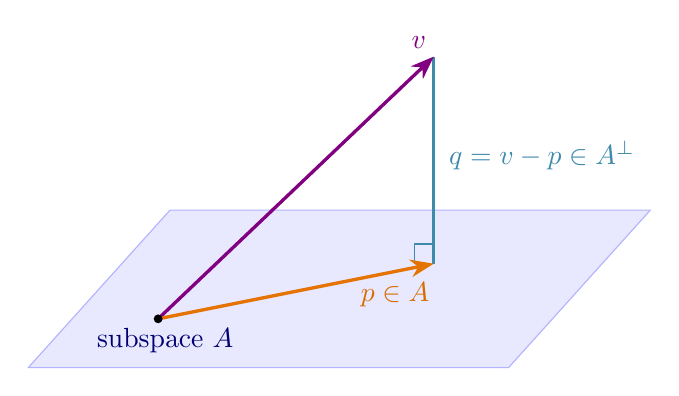
\begin{tikzpicture}[>=Stealth, line join=round]
\fill[blue!9]  (0,0) -- (6.1,0) -- (7.9,2.0) -- (1.8,2.0) -- cycle;
\draw[blue!30] (0,0) -- (6.1,0) -- (7.9,2.0) -- (1.8,2.0) -- cycle;
\coordinate (O) at (1.65,0.62);
\coordinate (P) at (5.15,1.32);
\coordinate (V) at (5.15,3.95);
\draw[very thick, cyan!65!black] (P) -- (V);
\draw[cyan!65!black] (4.90,1.32) -- (4.90,1.57) -- (5.15,1.57);
\draw[very thick, ->, violet]  (O) -- (V);
\draw[very thick, ->, orange!90!black] (O) -- (P);
\fill (O) circle (1.6pt);
\node[violet, above left=-1pt] at (V) {$v$};
\node[cyan!65!black, right=2pt] at (5.15,2.70) {$q=v-p\in A^{\perp}$};
\node[orange!85!black, below right=-2pt] at (4.15,1.15) {$p\in A$};
\node[blue!45!black, anchor=west] at (0.75,0.35) {subspace $A$};
\end{tikzpicture}
\caption{The orthogonal decomposition $V=A\oplus A^{\perp}$. Every $v$ splits
once and only once as $v=p+q$ with $p$ in the subspace $A$ and $q$
perpendicular to it. The right angle is the whole content of the theorem: $p$
is the point of $A$ nearest to $v$, which is why this decomposition is what
least squares approximation computes.}
\label{fig:orthogonal-decomposition}
\end{figure}

\begin{thm}\label{thm:row-column-rank}
If $A\in M_{m,n}(\mathbb{F})$, then the row rank of $A$ is equal to the column
rank of $A$.
\end{thm}

\begin{proof}
Let $r$ be the row rank of $A$, and let $u_1,\dots,u_r$ be a basis for the row
space, written as row vectors of length $n$. Every row of $A$ is a combination
of them, say
$$A_{i\bullet}=\sum_{k=1}^{r}c_{ik}u_k\qquad (i=1,\dots,m).$$
Reading this entry by entry, the $(i,j)$ entry of $A$ is
$$a_{ij}=\sum_{k=1}^{r}c_{ik}(u_k)_j.$$
Now fix $j$ and read the same identity \emph{down} the $j$-th column:
$$A_{\bullet j}=\sum_{k=1}^{r}(u_k)_j\,C_{\bullet k},$$
where $C=(c_{ik})$ is $m$ by $r$. This says every column of $A$ is a linear
combination of the $r$ columns of $C$. Hence the column space is spanned by $r$
vectors, and by the exchange lemma
$$\text{column rank of } A\leq r=\text{row rank of } A.$$

Applying this inequality to $A^t$, whose rows are the columns of $A$ and whose
columns are the rows of $A$, gives the reverse inequality
$$\text{row rank of } A\leq \text{column rank of } A.$$
The two together give equality.
\end{proof}

\begin{remark}
Because the two ranks agree, one may speak simply of \emph{the} rank of $A$.
This is not a formality: it is why the number of leading ones found by row
reducing $A$ --- a row computation --- also answers questions about the columns,
such as how many of them are linearly independent.
\end{remark}


\begin{defn}
Let $A$ be a squared matrix. Then $A$ is called
\begin{enumerate}
\item[i.] Orthogonal if $A^{-1}=A^{\perp}$ and $A$ is real.
\item[ii.] Unitary if $A^{-1}=A^{\perp}$ and $A$ is complex.\\
\end{enumerate}
\end{defn}



\begin{remark}
$A^{-1}=A^{\perp}\implies AA^{\perp}=I$\\
\end{remark}



\begin{thm}
Let $A$ be a square matrix. Then the following are equivalent,
\begin{enumerate}
\item[i.] $A$ is orthogonal/unitary.
\item[ii.] The columns of $A$ from an orthonormal set.
\item[iii.] The rows of $A$ form an orthonormal set.\\
\end{enumerate}
\end{thm}



\begin{proof}
Follows from $AA^{-1}=I$.\\
\end{proof}



\begin{exa}
$A=
\begin{pmatrix}
\cos{\theta}&-\sin{\theta}\\\sin{\theta}&\cos{\theta}\\
\end{pmatrix}
$
is an orthogonal matrix. Since the rows and columns are orthogonal to each other are are unit.\\
\end{exa}



\begin{defn}
A real symmetric matrix $A$ is called positive definite if $X\in \mathbb{R}^n$, then $(XAX)=X^tAX>0$.\\
\end{defn}


\begin{remark}
If $A$ is a $2\times 2$ matrix then its positive definite if $|A|>0$.\\
\end{remark}



\begin{exa}
Verify if $(X,Y)=x_1y_1-x_1y_2-x_2y_1+3x_2y_2$ is an inner product on $\mathbb{R}$, where $X=(x_1,x_2)$ and $Y=(y_1,y_2)$\\
\end{exa}



\begin{solution}
$(X,Y)=(X^tAY)=(x_1,x_2)
\begin{pmatrix}
1&-1\\-1&3\\
\end{pmatrix}
\begin{pmatrix}
y_1\\y_2\\
\end{pmatrix}
$\\
Now
$
\begin{vmatrix}
1&-1\\-1&3\\
\end{vmatrix}
=3-1=2>0$.\\
$\implies (X,Y)$ is an inner product.\\



\pagebreak
\end{solution}










 
\subsection*{Practice Problems}
\addcontentsline{toc}{subsection}{Practice Problems}

\begin{problem}
Let $x=(1,0,2)$ and $y=(2,1,2)$ in $\mathbb{R}^3$ with the standard inner
product. Compute $\|x\|$, $\|y\|$, $\|x+y\|$, $(x,y)$ and the angle between
$x$ and $y$; then verify the Cauchy--Schwarz and triangle inequalities.
\end{problem}
\begin{solution}
The inner product is $(x,y)=1\cdot 2+0\cdot 1+2\cdot 2=6$, and
$$\|x\|=\sqrt{1+0+4}=\sqrt5,\qquad \|y\|=\sqrt{4+1+4}=3,$$
while $x+y=(3,1,4)$ gives $\|x+y\|=\sqrt{9+1+16}=\sqrt{26}$.

The angle $\theta$ satisfies
$$\cos\theta=\frac{(x,y)}{\|x\|\,\|y\|}=\frac{6}{3\sqrt5}=\frac{2}{\sqrt5}
\approx 0.894,$$
so $\theta\approx 26.6^{\circ}$.

\subhead{Cauchy--Schwarz}
$|(x,y)|=6$ and $\|x\|\|y\|=3\sqrt5\approx 6.708$, so $6\leq 6.708$ holds.
Equality would mean $x$ and $y$ are parallel; they are not.

\subhead{Triangle inequality}
$\|x+y\|=\sqrt{26}\approx 5.099$ and $\|x\|+\|y\|=\sqrt5+3\approx 5.236$, so
$5.099\leq 5.236$ holds.
\end{solution}

\begin{problem}
Prove that in a real inner product space,
$$4(x,y)=\|x+y\|^2-\|x-y\|^2 \quad\text{and}\quad
\|x+y\|^2+\|x-y\|^2=2\left(\|x\|^2+\|y\|^2\right).$$
\end{problem}
\begin{solution}
Expand both norms using $\|v\|^2=(v,v)$ and bilinearity. In a \emph{real} space
$(x,y)=(y,x)$, so
$$\|x+y\|^2=(x+y,x+y)=\|x\|^2+2(x,y)+\|y\|^2,$$
$$\|x-y\|^2=(x-y,x-y)=\|x\|^2-2(x,y)+\|y\|^2.$$
Subtracting the second from the first, the $\|x\|^2$ and $\|y\|^2$ terms cancel
and the cross terms add:
$$\|x+y\|^2-\|x-y\|^2=4(x,y).$$
Adding them instead, the cross terms cancel and the rest doubles:
$$\|x+y\|^2+\|x-y\|^2=2\|x\|^2+2\|y\|^2.$$
The first identity says the inner product is recoverable from the norm alone;
the second, the \emph{parallelogram law}, is the test for whether a given norm
comes from an inner product at all.
\end{solution}

\begin{problem}
Suppose $\|x\|=3$, $\|x+y\|=4$ and $\|x-y\|=6$ in a real inner product space.
What must $\|y\|$ be?
\end{problem}
\begin{solution}
Apply the parallelogram law from the previous problem:
$$\|x+y\|^2+\|x-y\|^2=2\left(\|x\|^2+\|y\|^2\right).$$
Substituting the given values,
$$16+36=2(9+\|y\|^2)\implies 52=18+2\|y\|^2\implies \|y\|^2=17,$$
so $\|y\|=\sqrt{17}$. Note the data are not free: any norm satisfying the
parallelogram law determines $\|y\|$ once the other three are fixed.
\end{solution}

\begin{problem}
Show that there is no inner product on $\mathbb{R}^2$ whose associated norm is
$\|(x,y)\|=|x|+|y|$.
\end{problem}
\begin{solution}
If such an inner product existed, its norm would have to satisfy the
parallelogram law. Test it on $u=(1,0)$ and $v=(0,1)$:
$$\|u\|=1,\qquad \|v\|=1,$$
$$u+v=(1,1)\implies \|u+v\|=2,\qquad u-v=(1,-1)\implies \|u-v\|=2.$$
Then
$$\|u+v\|^2+\|u-v\|^2=4+4=8,$$
but
$$2\left(\|u\|^2+\|v\|^2\right)=2(1+1)=4.$$
Since $8\neq 4$ the parallelogram law fails, so this norm cannot arise from any
inner product.
\end{solution}

\begin{problem}
Find $c$ so that $x=(1,3,2,c)$ is orthogonal to $y=(3,1,-4,1)$ in
$\mathbb{R}^4$. Then find $c$ so that
$(x,y)=x_1y_1-3x_1y_2-3x_2y_1+cx_2y_2$ is an inner product on $\mathbb{R}^2$.
\end{problem}
\begin{solution}
\subhead{Orthogonality}
$$(x,y)=1\cdot 3+3\cdot 1+2\cdot(-4)+c\cdot 1=3+3-8+c=c-2,$$
which vanishes when $c=2$.

\subhead{The inner product}
The form has matrix $A=\begin{pmatrix}1&-3\\-3&c\end{pmatrix}$, since
$(x,y)=x^tAy$. It is symmetric and bilinear whatever $c$ is, so the only
condition to impose is positive definiteness: $(x,x)>0$ for $x\neq 0$.
Completing the square,
$$(x,x)=x_1^2-6x_1x_2+cx_2^2=(x_1-3x_2)^2+(c-9)x_2^2.$$
If $c>9$ this is a sum of two non-negative terms which vanish together only
when $x_2=0$ and $x_1=3x_2=0$, so it is positive definite. If $c\leq 9$, taking
$x=(3,1)$ gives $(x,x)=0+(c-9)\leq 0$ with $x\neq 0$, so it fails.

Hence the form is an inner product exactly when $\boldsymbol{c>9}$.
\end{solution}

\begin{problem}
Suppose $y\neq 0$ and $x$ is any vector in an inner product space. Show that
$$c=\frac{(x,y)}{\|y\|^2}$$
is the unique scalar for which $x'=x-cy$ is orthogonal to $y$.
\end{problem}
\begin{solution}
Compute the inner product of $x'=x-cy$ with $y$, using linearity in the first
argument:
$$(x',y)=(x-cy,\ y)=(x,y)-c(y,y)=(x,y)-c\|y\|^2.$$
This is zero if and only if $c\|y\|^2=(x,y)$, and since $y\neq 0$ we have
$\|y\|^2\neq 0$, so we may divide:
$$c=\frac{(x,y)}{\|y\|^2}.$$
The calculation gives existence and uniqueness at once --- the condition is a
single linear equation in $c$ with a non-zero coefficient.

The vector $cy$ is the orthogonal projection of $x$ onto the line spanned by
$y$, and this is exactly the step repeated at each stage of the Gram--Schmidt
procedure.
\end{solution}

\begin{problem}
Let $U$ be a subspace of a finite dimensional inner product space $V$. Prove
that $\dim U^{\perp}=\dim V-\dim U$, and deduce that $U^{\perp}=\{0\}$ if and
only if $U=V$.
\end{problem}
\begin{solution}
By Theorem~\ref{thm:orthogonal-decomposition}, $V=U\oplus U^{\perp}$. For a
direct sum the dimensions add: taking a basis of $U$ and a basis of
$U^{\perp}$, their union spans $V$ because every vector decomposes, and it is
independent because a dependence would give a non-zero vector in
$U\cap U^{\perp}=\{0\}$. Hence
$$\dim V=\dim U+\dim U^{\perp},$$
which rearranges to the stated formula.

For the consequence: $U^{\perp}=\{0\}$ means $\dim U^{\perp}=0$, which by the
formula holds exactly when $\dim U=\dim V$; and a subspace of the same finite
dimension as the whole space is the whole space. So $U^{\perp}=\{0\}$ if and
only if $U=V$.
\end{solution}

\begin{problem}
What happens if the Gram--Schmidt procedure is applied to a list of vectors
that is not linearly independent?
\end{problem}
\begin{solution}
The procedure breaks down at the first vector that is a combination of its
predecessors, and it does so in a visible way: that step produces the zero
vector, which cannot then be normalised.

Concretely, at step $k$ Gram--Schmidt forms
$$w_k=v_k-\sum_{i<k}(v_k,e_i)e_i,$$
the part of $v_k$ orthogonal to the span of $v_1,\dots,v_{k-1}$. If $v_k$
already lies in that span then subtracting its projection removes all of it and
$w_k=0$. The next instruction, $e_k=w_k/\|w_k\|$, then divides by zero.

So the procedure is self-diagnosing: it is a test for independence as well as a
method of orthogonalisation. The usual repair is to discard any $v_k$ producing
$w_k=0$ and carry on, which yields an orthonormal basis for the span of the
original list rather than one vector per input.
\end{solution}

\pagebreak
\section{CHARACTERISTIC ROOTS AND VECTORS}



\subsection{Eigenvalues and Vectors}


\begin{defn}
Let $A\in M_n(\mathbb{F})$. Then $\lambda \in \mathbb{F}$ is called an eigenvalue of $A$ if $\exists$ a non zero vector $X\in V_n(\mathbb{F})$ such that $AX=\lambda X$.\\ The $X$ here is called an eigenvector corresponding to $\lambda$.\\
\end{defn}



\begin{defn}
Let $V$ be a finite dimensional vector space and $T\in \mathcal{L}(V)$. Then $\lambda \in \mathbb{F}$ is called an eigenvalue of $T$ if $\exists X\in V, X\neq 0$ such that $TX=\lambda X$, $X$ is corresponding eigenvector.
\begin{align*}
\text{From}\hspace{0.5cm} AX &=\lambda X\\
                          AX-\lambda X &=0\\
                          (A-\lambda I)X &=0\hspace{0.3cm}\text{where}\hspace{0.3cm} I\hspace{0.3cm}\text{is identity matrix}.
\end{align*}
Since $X\neq 0$ then $A-\lambda I=0\implies \det (A-\lambda I)=0$.\\
\end{defn}




\begin{thm}\label{thm:eigen-det}
$\lambda \in \mathbb{F}$ is an eigenvalue of $A$ if and only if
$\det (A-\lambda I)=0$.
\end{thm}

\begin{proof}
By definition $\lambda$ is an eigenvalue of $A$ exactly when there is a
\emph{non-zero} vector $x$ with $Ax=\lambda x$, that is
$$(A-\lambda I)x=0.$$
So $\lambda$ is an eigenvalue if and only if the homogeneous system with
coefficient matrix $A-\lambda I$ has a non-trivial solution. By the $n$ by $n$
determinant theorem, part (4), that happens if and only if
$\det(A-\lambda I)=0$.

The insistence on $x\neq 0$ is what makes the statement have content: $x=0$
satisfies $Ax=\lambda x$ for every $\lambda$ whatsoever, so admitting it would
make every scalar an eigenvalue.
\end{proof}



\begin{defn}
The characteristic polynomial of matrix $A$ is $X_A(x)=\det (A-xI)$.\\
\end{defn}



\begin{thm}\label{thm:eigen-char-poly}
$\lambda \in \mathbb{F}$ is an eigenvalue of $A$ if and only if it is a root of
the characteristic polynomial $X_A(x)$.
\end{thm}

\begin{proof}
The characteristic polynomial is defined by $X_A(x)=\det(A-xI)$. So
$$X_A(\lambda)=0 \iff \det(A-\lambda I)=0 \iff \lambda \text{ is an
eigenvalue of } A,$$
the second equivalence being Theorem~\ref{thm:eigen-det}.

This converts the search for eigenvalues, which as stated is a search over all
of $\mathbb{F}$ for scalars admitting a non-zero solution, into the finite
problem of factoring a polynomial of degree $n$. In particular an $n$ by $n$
matrix has at most $n$ distinct eigenvalues.
\end{proof}



\begin{exa}\label{exa:eigen-example}
Find the eigenvalues and vectors of $
A=
\begin{pmatrix}
4&2\\3&-1\\
\end{pmatrix}
$.\\
\end{exa}



\begin{solution}
$\lambda$ is eigenvalue if and only if it is root of $|A-x\lambda|=0$.\\\\
Now $|A-xI|=0$
\begin{align*}
\begin{vmatrix}
4-x&2\\3&-1-x\\
\end{vmatrix}
&=0\\\\
(4-x)(-1-x)-6 &=0\\
-4-4x+x+x^2-6 &=0\\\\
x^2-3x-10 &=0\\
x^2-5x+2x-10 &=0\\
(x-5)(x+2) &=0\\\\
\implies \hspace{0.4cm} x&=5, -2
\end{align*}
i.e. eigenvalues are $\lambda_1=5$ and $\lambda_2=-2$.\\\\
If $\lambda=5$ then $(A-\lambda I)=0$
\begin{align*}
\begin{pmatrix}
4-\lambda_1 &2\\3&-1-\lambda_1\\
\end{pmatrix}
\begin{pmatrix}
x_1\\x_2\\
\end{pmatrix}
&=
\begin{pmatrix}
0\\0\\
\end{pmatrix}\\\\
\begin{pmatrix}
-1&2\\3&-6\\
\end{pmatrix}
\begin{pmatrix}
x_1\\x_2\\
\end{pmatrix}
&=
\begin{pmatrix}
0\\0\\
\end{pmatrix}
\end{align*}
$-x_1+2x_2=0\implies x_1=2x_2\implies x_1=2$ if $x_2=1$.\\\\
Therefore, if $\lambda=5$ then $
\begin{pmatrix}
x_1\\x_2\\
\end{pmatrix}
=
\begin{pmatrix}
2\\1\\
\end{pmatrix}
$.\\\\
Now if $\lambda=-2$ then
\begin{align*}
\begin{pmatrix}
4+2&2\\3&-1+2\\
\end{pmatrix}
\begin{pmatrix}
x_1\\x_2\\
\end{pmatrix}
&=
\begin{pmatrix}
0\\0\\
\end{pmatrix}\\\\
\begin{pmatrix}
6&2\\3&1\\
\end{pmatrix}
\begin{pmatrix}
x_1\\x_2\\
\end{pmatrix}
&=
\begin{pmatrix}
0\\0\\
\end{pmatrix}
\end{align*}
$6x_1+2x_2=0\implies x_2=-3x_1\implies x_2=-3$ if $x_1=1$.\\\\
Therefore, if $\lambda=-2$ then $
\begin{pmatrix}
x_1\\x_2\\
\end{pmatrix}
=
\begin{pmatrix}
1\\-3\\
\end{pmatrix}
$.\\\\


Recall that if $A,B\in M_n(\mathbb{F})$, then $A$ is similar to matrix $B$ if there exists an invertible matrix $P\in M_n(\mathbb{F})\ni B=P^{-1}AP$.\\\\
\end{solution}
\begin{lem}\label{lem:similar-char-poly}
Similar matrices have the same characteristic polynomial, and hence the same
eigenvalues.
\end{lem}

\begin{proof}
Suppose $B=P^{-1}AP$ with $P$ invertible. Then, using $P^{-1}IP=I$,
$$B-xI=P^{-1}AP-xP^{-1}IP=P^{-1}(A-xI)P.$$
Taking determinants and using the multiplicative property,
$$X_B(x)=\det(B-xI)=\det(P^{-1})\det(A-xI)\det(P)
=\frac{1}{\det P}\det(A-xI)\det P=\det(A-xI)=X_A(x).$$
So the two characteristic polynomials are identical, and by
Theorem~\ref{thm:eigen-char-poly} their roots --- the eigenvalues --- coincide.

Note the order of the statement: equality of the characteristic polynomials is
the stronger fact, and the equality of eigenvalues follows from it, not the
other way round.
\end{proof}


\begin{defn}
If $T\in \mathcal{L}(V)$, then the characteristic polynomial of $T$ is the characteristic of the matrix of $T$ relative to any basis for $V$.\\ The set $V(\lambda)$ of eigenvectors corresponding to eigenvalue together with zero is a subspace of $V_n(\mathbb{F})$ and is called the eigen space corresponding to $\lambda$.\\\\
\end{defn}




\subsection{Diagonalization of Matrices and Linear Transformations}

\begin{defn}
A matrix $A\in M_n(\mathbb{F})$ is diagonalizable if $\exists$ an invertible matrix $P$ such that $P^{-1}AP$ is a diagonal matrix.\\
\end{defn}



\begin{defn}
A linear transformation $T\in \mathcal{L}(V)$ is diagonalizable if there exist an $\mathbb{F}-$basis for $V$ such that the matrix of $T$ relative to this basis is diagonal matrix.\\\\


\end{defn}
The following theorem provides sufficient conditions for diagonalization.\\


\begin{thm}\label{thm:diagonalizable-criterion}
Let $A\in M_n(\mathbb{F})$. Then
\begin{enumerate}
\item[i.] $A$ is diagonalizable if and only if its \emph{eigenvectors} include a
basis for $V_n(\mathbb{F})$;
\item[ii.] $A$ is diagonalizable if it has $n$ distinct eigenvalues.
\end{enumerate}
\end{thm}

\begin{proof}
\begin{enumerate}
\item[i.] Suppose $A$ is diagonalizable, so $P^{-1}AP=D$ with $D$ diagonal,
say with diagonal entries $d_1,\dots,d_n$. Rewriting, $AP=PD$. Comparing the
$j$-th columns, and writing $p_j$ for the $j$-th column of $P$,
$$Ap_j=d_jp_j.$$
Each $p_j$ is non-zero because $P$ is invertible, so each $p_j$ is an
eigenvector with eigenvalue $d_j$; and the columns of an invertible matrix are
linearly independent, so $\{p_1,\dots,p_n\}$ is a basis.

Conversely, suppose there is a basis $\{p_1,\dots,p_n\}$ consisting of
eigenvectors, $Ap_j=d_jp_j$. Let $P$ be the matrix with these as columns. It is
invertible, its columns being a basis, and the computation above run backwards
gives $AP=PD$, that is $P^{-1}AP=D$.

\item[ii.] It suffices, by (i), to show that eigenvectors belonging to distinct
eigenvalues are linearly independent; $n$ of them then form a basis, since
$\dim V_n(\mathbb{F})=n$.

Let $v_1,\dots,v_k$ be eigenvectors for distinct eigenvalues
$\lambda_1,\dots,\lambda_k$ and suppose they are dependent. Among all
non-trivial relations choose one with the fewest non-zero coefficients, say
$$c_1v_1+c_2v_2+\cdots+c_mv_m=0$$
after renumbering, with every $c_i\neq 0$ and $m\geq 2$ (a single term
$c_1v_1=0$ with $c_1\neq 0$ would force $v_1=0$, which no eigenvector is).
Apply $A-\lambda_mI$ to both sides. Since $(A-\lambda_mI)v_i
=(\lambda_i-\lambda_m)v_i$, this gives
$$c_1(\lambda_1-\lambda_m)v_1+\cdots+c_{m-1}(\lambda_{m-1}-\lambda_m)v_{m-1}=0.$$
The eigenvalues are distinct, so every coefficient $c_i(\lambda_i-\lambda_m)$
with $i<m$ is non-zero --- yet this relation has one fewer term, contradicting
minimality. Hence the eigenvectors are independent.
\end{enumerate}
\end{proof}

\begin{remark}
The converse of (ii) is false: $A=I$ is diagonalizable (it is already diagonal)
but has only the single eigenvalue $1$. Distinct eigenvalues are sufficient for
diagonalizability, never necessary.
\end{remark}


\begin{remark}
\begin{enumerate}
\item Condition: (1) implies that if $A$ is diagonalizable then $X_A(x)$ factors completely into linear factors.
\item $P^{-1}AP= $diag$(\lambda_1,\lambda_2,\dots,\lambda_n)$ where $\lambda_i$ are eigenvalues of $A$.
\item This also apply to LTS.\\
\end{enumerate}
\end{remark}




\begin{exa}
Consider the matrix $A=
\begin{pmatrix}
4&2\\3&-1\\
\end{pmatrix}
$. Determine if $A$ is diagonalizable and find $P^{-1}AP$.\\
\end{exa}



\begin{solution}
From Example~\ref{exa:eigen-example} the eigenvalues are $\lambda_1=5$, $\lambda_2=-2$. i.e. two distinct eigenvalues for $2\times 2$ matrix.\\\\
$\implies A$ is diagonalizable.\\\\
Now, $P^{-1}AP=$ diag$(\lambda_1,\lambda_2)=$ diag$(5,-2)=
\begin{pmatrix}
5&0\\0&-2\\
\end{pmatrix}
$.\\\\
We can find $P$, since $\{(2,1)\}$ is a basis for $V(5)$ and $\{(1,-3)\}$ is a basis for $V(-2)$ then $P=
\begin{pmatrix}
2&1\\1&-3\\
\end{pmatrix}
$  and indeed
$$ P^{-1}AP=
\begin{pmatrix}
2&1\\1&-3\\
\end{pmatrix}^{-1}
\begin{pmatrix}
4&2\\3&-1\\
\end{pmatrix}
\begin{pmatrix}
2&1\\1&-3\\
\end{pmatrix}
=\begin{pmatrix}
5&0\\0&2\\
\end{pmatrix}
=\text{diag}(\lambda_1,\lambda_2)
$$
\end{solution}


\begin{defn}
A minimum polynomial of a matrix $A\in M_n(\mathbb{F})$ is the monic polynomial $M(x)$ of least degree such that $M(A)=0$.\\ Such a polynomial is of degree at most $n^2$.\\

\end{defn}
 We now look at some properties of this polynomial.\\




\begin{lem}
The minimum polynomial of $A\in M_n(\mathbb{F})$ is unique.\\
\end{lem}




\begin{proof}
Let $M(x)$ and $M'(x)$ be minimum polynomial of $A$.\\ $\implies \deg(M(x))=\deg (M'(x))$.\\ Define $f(x)=M(x)-M'(x)$ then $\deg (f(x))<\deg (M(x))$ or $\deg (M'(x))$. Since $M(x)$ and $M'(x)$ are Monic.\\ Now $f(A)=M(A)-M'(A)=0-0=0$ and so $f(x)$ is monic.\\ Therefore $f(x)$ is a minimum polynomial with $\deg (f(x))<\deg (M(x))$ a contradiction. So $f$ does not exist and $M(x)=M'(x)$.\\
\end{proof}




\begin{lem}\label{lem:min-poly-divides}
The minimum polynomial $M(x)$ of $A\in M_n(\mathbb{F})$ divides every polynomial $f(x)$ with $f(A)=0$.\\
\end{lem}



\begin{proof}
By division algorithm the exist polynomials $q(x)$ and $r(x)$ such that $f(x)=q(x)M(x)+r(x)$ where $\deg (r(x))<\deg (M(x))$ or $r(x)=0$. Now,
\begin{align*}
r(A) &=f(A)-q(A)M(A)\\
     &=0-q(A)(0)\\
     &=0-0\\
     &=0
\end{align*}
Suppose $\deg (r(x))\geq 1$, then $r(x)$ is minimum with $\deg (r(x))<\deg (M(x))$ a contradiction, since minimum polynomial is unique. Thus $r(x)=0$ and $f(x)=q(x)M(x)$ $$\implies M(x)=\frac{f(x)}{q(x)}$$\\
\end{proof}



\begin{lem}\label{lem:similar-min-poly}
Similar matrices have the same minimum polynomial.
\end{lem}

\begin{proof}
Let $B=P^{-1}AP$. First note that powers behave well under similarity:
$$B^k=(P^{-1}AP)^k=P^{-1}A^kP,$$
because the interior factors $PP^{-1}$ cancel in pairs. Consequently, for any
polynomial $f(x)=\sum_k a_kx^k$,
$$f(B)=\sum_k a_kB^k=\sum_k a_kP^{-1}A^kP=P^{-1}\left(\sum_k a_kA^k\right)P
=P^{-1}f(A)P.$$
Since $P$ is invertible, $f(B)=0$ if and only if $f(A)=0$. So $A$ and $B$ are
annihilated by exactly the same polynomials, and in particular the monic
polynomial of least degree annihilating one annihilates the other. Hence their
minimum polynomials agree.
\end{proof}





\subsection{Cayley-Hamilton theorem}
\begin{thm}[Cayley-Hamilton theorem]\label{thm:cayley-hamilton}
Every matrix $A$ is a root of its characteristic polynomial, that is
$X_A(A)=0$.
\end{thm}

\begin{proof}
It is tempting to ``prove'' this by substituting $x=A$ into $X_A(x)=\det(A-xI)$
to get $\det(A-A)=0$. That argument is wrong: $X_A(x)$ is a scalar polynomial,
and replacing the scalar $x$ by a matrix inside a determinant is not a
legitimate operation. A genuine proof uses the adjoint.

The entries of $\text{adj}(A-xI)$ are determinants of $(n-1)$ by $(n-1)$
submatrices of $A-xI$, hence polynomials in $x$ of degree at most $n-1$.
Collecting powers of $x$, we may therefore write
$$\text{adj}(A-xI)=B_0+B_1x+B_2x^2+\cdots+B_{n-1}x^{n-1}$$
for some constant matrices $B_0,\dots,B_{n-1}$.

The identity established in the proof of Theorem~\ref{thm:adjoint-inverse}
gives
$$(A-xI)\,\text{adj}(A-xI)=\det(A-xI)\,I=X_A(x)\,I.$$
Write $X_A(x)=c_0+c_1x+\cdots+c_nx^n$ and expand the left-hand side:
$$(A-xI)\sum_{k=0}^{n-1}B_kx^k
=\sum_{k=0}^{n-1}AB_kx^k-\sum_{k=0}^{n-1}B_kx^{k+1}.$$
Two polynomials in $x$ with matrix coefficients are equal only if
corresponding coefficients agree, so
$$AB_0=c_0I,\qquad AB_k-B_{k-1}=c_kI \ \ (1\leq k\leq n-1),\qquad
-B_{n-1}=c_nI.$$

Now multiply the $k$-th of these on the left by $A^k$ and add them all:
$$AB_0+\sum_{k=1}^{n-1}\left(A^{k+1}B_k-A^kB_{k-1}\right)-A^nB_{n-1}
=c_0I+\sum_{k=1}^{n-1}c_kA^k+c_nA^n.$$
The left-hand side telescopes --- $AB_0$ cancels against $-A^1B_0$, then
$A^2B_1$ against $-A^2B_1$, and so on --- leaving $0$. The right-hand side is
exactly $X_A(A)$. Hence $X_A(A)=0$.
\end{proof}

\begin{remark}
One practical consequence: for an invertible $A$, the relation
$c_0I+c_1A+\cdots+c_nA^n=0$ can be rearranged to express $A^{-1}$ as a
polynomial in $A$, since $c_0=\det A\neq 0$. Powers $A^k$ with $k\geq n$ can
likewise be reduced to combinations of $I,A,\dots,A^{n-1}$.
\end{remark}




\begin{exa}
Verify the Cayley-Halmiton theorem given $A=
\begin{pmatrix}
1&3\\4&5\\
\end{pmatrix}
$.\\
\end{exa}




\begin{solution}
\begin{align*}
X_A(x) &=
\begin{vmatrix}
1-x&3\\4&5-x\\
\end{vmatrix}\\\\
&=(1-x)(5-x)-12\\
&=x^2-6x-7
\end{align*}
Now
\begin{align*}
X_A(A) &=A^2-6A-7I\\
&=
\begin{pmatrix}
1&3\\4&5\\
\end{pmatrix}
\begin{pmatrix}
1&3\\4&5\\
\end{pmatrix}
-6
\begin{pmatrix}
1&3\\4&5\\
\end{pmatrix}
-7
\begin{pmatrix}
1&0\\0&1\\
\end{pmatrix}\\\\
&=
\begin{pmatrix}
0&0\\0&0\\
\end{pmatrix}\\
\end{align*}
\end{solution}





\begin{coro}
The minimum polynomial divides associated characteristics polynomial.\\
\end{coro}



\begin{proof}
Follows directly from Theorem~\ref{thm:cayley-hamilton} and Lemma~\ref{lem:min-poly-divides}.\\
\end{proof}





\begin{thm}\label{thm:min-char-factors}
The distinct linear factors of the minimum polynomial coincide with those of
the characteristic polynomial.
\end{thm}

\begin{proof}
Both directions amount to showing that the roots of $M(x)$ are exactly the
eigenvalues of $A$, since by Theorem~\ref{thm:eigen-char-poly} the roots of
$X_A(x)$ are the eigenvalues.

\subhead{Every eigenvalue is a root of $M$}
Let $\lambda$ be an eigenvalue with eigenvector $v\neq 0$. Then $Av=\lambda v$,
and applying $A$ repeatedly gives $A^kv=\lambda^kv$, so for any polynomial $f$,
$$f(A)v=f(\lambda)v.$$
Taking $f=M$ and using $M(A)=0$ gives $M(\lambda)v=0$. As $v\neq 0$, this
forces $M(\lambda)=0$.

\subhead{Every root of $M$ is an eigenvalue}
Let $M(\lambda)=0$ and factor $M(x)=(x-\lambda)g(x)$. Since $\deg g<\deg M$ and
$M$ has least degree among monic annihilating polynomials, $g(A)\neq 0$. So
there is a vector $v$ with $w=g(A)v\neq 0$. Then
$$(A-\lambda I)w=(A-\lambda I)g(A)v=M(A)v=0,$$
so $w$ is a non-zero vector with $Aw=\lambda w$, that is, $\lambda$ is an
eigenvalue.

The two halves together show the roots of $M$ and of $X_A$ form the same set,
so the distinct linear factors coincide.
\end{proof}




\begin{coro}\label{coro:min-poly-diagonalizable}
If a matrix $A\in M_n(\mathbb{F})$ has $n$ distinct eigenvalues then its minimum
and characteristic polynomials coincide. More generally, a matrix with $k$
distinct eigenvalues $\lambda_1,\dots,\lambda_k$ is diagonalizable if and only
if its minimum polynomial is
$$M(x)=(x-\lambda_1)(x-\lambda_2)\cdots(x-\lambda_k),$$
that is, if and only if $M$ has no repeated factor.
\end{coro}

\begin{proof}
Suppose first that $A$ has $n$ distinct eigenvalues. By
Theorem~\ref{thm:min-char-factors} the minimum polynomial has all $n$ of them
as roots, so it is divisible by $(x-\lambda_1)\cdots(x-\lambda_n)$ and therefore
has degree at least $n$. On the other hand $M$ divides $X_A$, by
Theorem~\ref{thm:cayley-hamilton} together with
Lemma~\ref{lem:min-poly-divides}, so $\deg M\leq n$. Hence $\deg M=n$; being
monic, of the same degree as $X_A$, and a divisor of it, $M=X_A$.

For the general statement, suppose $A$ is diagonalizable, so it is similar to a
diagonal matrix $D$ carrying the $\lambda_i$ on its diagonal. By
Lemma~\ref{lem:similar-min-poly} similar matrices share a minimum polynomial,
so it suffices to compute that of $D$. For diagonal $D$, $f(D)$ is diagonal
with entries $f(\lambda_i)$, so $f(D)=0$ exactly when $f$ vanishes at every
$\lambda_i$. The monic polynomial of least degree doing so is
$(x-\lambda_1)\cdots(x-\lambda_k)$, which is therefore the minimum polynomial.

Conversely, suppose $M(x)=(x-\lambda_1)\cdots(x-\lambda_k)$ with the
$\lambda_i$ distinct. For each $i$ put
$g_i(x)=\prod_{j\neq i}(x-\lambda_j)$. These $k$ polynomials have no common
root, so their greatest common divisor is $1$ and there are polynomials $h_i$
with $\sum_i h_ig_i=1$. Substituting $A$,
$$\sum_{i=1}^{k}h_i(A)g_i(A)=I,$$
so every $v$ decomposes as $v=\sum_i v_i$ with $v_i=h_i(A)g_i(A)v$. Each such
$v_i$ satisfies $(A-\lambda_iI)v_i=h_i(A)M(A)v=0$, so it is either $0$ or an
eigenvector for $\lambda_i$. Hence the eigenvectors span the whole space, and
by Theorem~\ref{thm:diagonalizable-criterion}(i) $A$ is diagonalizable.
\end{proof}



\begin{exa}
\begin{enumerate}
\item[i.] Find the minimum polynomial of $A=
\begin{pmatrix}
1&1&0&0\\0&1&0&0\\0&0&2&0\\0&0&0&2\\
\end{pmatrix}
$
\item[ii.] Is $A$ diagonalizable?\\
\end{enumerate}
\end{exa}



\begin{solution}
\begin{align*}
X_A(x) &=
\begin{vmatrix}
1-x&1&0&0\\0&1-x&0&0\\0&0&2-x&0\\0&0&0&2-x\\
\end{vmatrix}
=(2-x)
\begin{vmatrix}
1-x&1&0\\0&1-x&0\\0&0&2-x\\
\end{vmatrix}\\\\
&=(2-x)^x
\begin{vmatrix}
1-x&1\\0&1-x\\
\end{vmatrix}\\\\
&=(2-x)^2(1-x)^2\\
\end{align*}
By Theorem~\ref{thm:min-char-factors}, the minimum polynomial is one of 
\begin{enumerate}
\item[i.] $(x-2)(x-1)$
\item[ii.] $(x-2)^2(x-1)$
\item[iii.] $(x-2)(x-1)^2$
\item[iv.] $(x-2)^2(x-1)^2$
\end{enumerate}
So we start with i
\begin{align*}
f(A) &=(A-I)(A-2I)\\
&=
\begin{pmatrix}
0&1&0&0\\0&0&0&0\\0&0&1&0\\0&0&0&1\\
\end{pmatrix}
\begin{pmatrix}
-1&1&0\\0&-1&0\\0&0&0\\0&0&0\\
\end{pmatrix}\\\\
&=
\begin{pmatrix}
0&-1&0&0\\0&0&0&0\\0&0&0&0\\0&0&0&0\\0&0&0&0\\
\end{pmatrix}\\\\
&\neq 0\\
\end{align*}
ii it fails\\\\
Now, we check for iii
\begin{align*}
f(A) &=(A-I)^2(A-2I)\\
&=
\begin{pmatrix}
0&1&0&0\\0&0&0&0\\0&0&1&0\\0&0&0&1\\
\end{pmatrix}
\begin{pmatrix}
0&-1&0&0\\0&0&0&0\\0&0&0&0\\0&0&0&0\\
\end{pmatrix}\\\\
&=
\begin{pmatrix}
0&0&0&0\\0&0&0&0\\0&0&0&0\\0&0&0&0\\
\end{pmatrix}\\\\
&=0
\end{align*}
So $M(x)=(x-1)^2(x-2)$.
$\implies$ it is not diagonazable since the minimum and characteristic polynomial do not coincide $\implies$ $A$ is not diagonazable.\\\\
\end{solution}




\begin{exa}
Is $A=
\begin{pmatrix}
3&2&4\\2&0&2\\4&2&3\\
\end{pmatrix}
$ is diagonable?\\
\begin{align*}
X_A(x) &=
\begin{vmatrix}
3-x&2&4\\2&-x&2\\4&2&3-x\\
\end{vmatrix}\\\\
&=-(x+1)^2(x-8)=0\\\\
\implies\hspace{0.3cm} &\lambda_1=-1,\hspace{0.3cm}\lambda_2=8.
\end{align*}
Thus $A$ is diagonalizable if and only if $M(x)=(x+1)(x-8)$.\\
Now
\begin{align*}
M(A) &=(A+I)(A-8I)\\\\
&=\begin{pmatrix}
4&2&4\\2&1&2\\4&2&4\\
\end{pmatrix}
\begin{pmatrix}
-5&2&4\\2&-8&2\\4&2&-5\\
\end{pmatrix}
=0
\end{align*}
and so $A$ is diagonalizable.\\\\
\end{exa}





\subsection{Diagonalization of Symmetric Matrices}
A real matrix may not have real eigenvalues unless if it is symmetric $(A^T=A)$.\\\\ We denote the set of all real symmetric $n\times n$ matrices by $M^{(s)}_n(\mathbb{R})$.\\





\begin{defn}
$A,B\in M^{(s)}_n(\mathbb{R})$ are called orthogonally similar if there exist an orthogonal matrix $P\in M_n(\mathbb{R})$ such that $B=P^tAP$.\\
\end{defn}




\begin{lem}\label{lem:symmetric-real-eigenvalues}
The eigenvalues of a real symmetric matrix are real.
\end{lem}



\begin{proof}
Let $A\in M_n^{(s)}(\mathbb{R})$ and $\lambda$ be an eigenvalue of $A$ with corresponding vector $X\in V_n(\mathbb{R})$, then $AX=\lambda X\qquad (1)$.\\ From (1)
\begin{align*}
X^{-t}AX &=X^{-t}\lambda X\\
X^{-t}AX&=\lambda X^{-t}X\qquad (2)
\end{align*}
Also from (1)
\begin{align*}
\Big(\overline{A}\hspace{0.1cm}\overline{X}\Big)^t &=\Big(\overline{\lambda}\hspace{0.1cm}\overline{X}\Big)^t\\
\overline{X}^t\hspace{0.1cm}\overline{A}^t &=\overline{\lambda}^t\hspace{0.1cm}\overline{X}^t\\
\overline{X}^tA &=\overline{\lambda}\hspace{0.1cm}\overline{X}^t\\
\overline{X}^tAX &=\overline{\lambda}\hspace{0.1cm}\overline{X}^tX\qquad (3)
\end{align*}
From (1) and (2)
\begin{align*}
\lambda X^{-1}tX &=\overline{\lambda}\hspace{0.1cm}\overline{X}^tX\\
(\lambda-\overline{\lambda})\hspace{0.1cm}\overline{X}^tX &=0\\
\implies \hspace{0.3cm}(\lambda-\overline{\lambda})&=0\hspace{0.3cm}\text{since}\hspace{0.3cm}\overline{X}^tX\neq 0\\
\implies \hspace{0.3cm} \lambda &=\overline{\lambda}\\
\implies \hspace{0.3cm}\lambda \hspace{0.3cm}\text{is real}.\\
\end{align*}
\end{proof}




\begin{lem}
If the eigenvalues of a real symmetric matrix $A$ are distinct, then the corresponding eigen vectors are orthogonal to each other.\\
\end{lem}



\begin{proof}
Let $\lambda_1,\lambda_2,\dots,\lambda_n$ be the distinct eigenvalues of $A$ with corresponding eigen vectors $X_1,X_2,\dots,X_n$ respectively. Then
\begin{align*}
AX_i &=\lambda_iX_i,\hspace{0.5cm} i=1,2,\dots,n\\
X_i^tA &=\lambda_iX_i^t\\\\
X^t_iAX_j &=\lambda_iX^t_iX_j\qquad (1)
\end{align*}
Also
\begin{align*}
AX_j &=\lambda_j X_j\\
X^t_iAX_j &=X^t_i\lambda_iX_j=\lambda_jX_i^tX_j\qquad (2)
\end{align*}
(1) and (2) gives$$\lambda_jX_i^tX_j=\lambda_iX^t_iX_j\implies (\lambda_j-\lambda_i)X^t_iX_j=0$$
$\implies X^t_iX_j=0$ since $\lambda_i\neq \lambda_j$. Therefore $(X^t_i,X_j)=0\hspace{0.3cm} \forall i\neq j$. $\implies \hspace{0.3cm X_i\perp X_j}$.\\
\end{proof}




\begin{thm}
If $A$ is a real symmetric matrix with distinct eigenvalues then $A$ is
orthogonally similar to a diagonal matrix.
\end{thm}

\begin{proof}
Two facts about a real symmetric $A$ do the work.

\subhead{Eigenvectors for distinct eigenvalues are orthogonal}
Let $Av=\lambda v$ and $Aw=\mu w$ with $\lambda\neq\mu$. Using $A^t=A$,
$$\lambda (v,w)=(Av,w)=(v,A^tw)=(v,Aw)=\mu (v,w),$$
so $(\lambda-\mu)(v,w)=0$, and as $\lambda\neq\mu$ we get $(v,w)=0$.

\subhead{Assembling the matrix}
Since the eigenvalues are real and distinct, there are $n$ of them, with
eigenvectors $v_1,\dots,v_n$. Normalise each to unit length, $e_i=v_i/\|v_i\|$;
by the paragraph above the $e_i$ are pairwise orthogonal, so
$\{e_1,\dots,e_n\}$ is an orthonormal set of $n$ vectors and hence an
orthonormal basis.

Let $P$ be the matrix with columns $e_1,\dots,e_n$. Its columns being
orthonormal means precisely that $P^tP=I$, that is, $P$ is orthogonal and
$P^{-1}=P^t$. As in Theorem~\ref{thm:diagonalizable-criterion}(i), $AP=PD$ with
$D=\text{diag}(\lambda_1,\dots,\lambda_n)$, so
$$P^tAP=P^{-1}AP=D.$$
Thus $A$ is orthogonally similar to a diagonal matrix.
\end{proof}




\begin{thm}
If $A$ is a real symmetric matrix then there exists an orthogonal matrix $P$
such that $P^tAP=\text{diag}(\lambda_1,\lambda_2,\dots,\lambda_n)$, where
$\lambda_1,\dots,\lambda_n$ are the eigenvalues of $A$. \emph{(Spectral
theorem.)}
\end{thm}

\begin{proof}
The previous theorem assumed the eigenvalues were distinct. The point here is
that no such assumption is needed; the proof is by induction on $n$.

For $n=1$ there is nothing to prove. Suppose the result holds for symmetric
matrices of size $n-1$, and let $A$ be real symmetric of size $n$. By
Lemma~\ref{lem:symmetric-real-eigenvalues} its eigenvalues are real, so choose
one of them, $\lambda_1$, with a unit eigenvector $e_1$.

Let $W=\{x:(x,e_1)=0\}$ be the orthogonal complement of $e_1$; by
Theorem~\ref{thm:orthogonal-decomposition}, $\mathbb{R}^n=\langle e_1\rangle
\oplus W$ and $\dim W=n-1$. The key observation is that $A$ maps $W$ into
itself: if $(x,e_1)=0$ then, using symmetry,
$$(Ax,e_1)=(x,Ae_1)=(x,\lambda_1e_1)=\lambda_1(x,e_1)=0,$$
so $Ax\in W$.

Choose an orthonormal basis of $W$ and let $A'$ be the matrix of the
restriction of $A$ to $W$ in that basis. $A'$ is symmetric --- it is the matrix
of a map satisfying $(Ax,y)=(x,Ay)$ with respect to an orthonormal basis --- and
has size $n-1$, so by the induction hypothesis $W$ has an orthonormal basis
consisting of eigenvectors of $A$. Adjoining $e_1$ gives an orthonormal basis
$e_1,\dots,e_n$ of $\mathbb{R}^n$ made of eigenvectors of $A$.

Let $P$ have these as its columns. Then $P^tP=I$, so $P$ is orthogonal, and
$AP=PD$ gives $P^tAP=D=\text{diag}(\lambda_1,\dots,\lambda_n)$.
\end{proof}

\begin{remark}
This is the strongest diagonalization result in the course, and its two extra
conclusions matter: the diagonalizing matrix can be taken \emph{orthogonal}, so
that $P^{-1}$ costs nothing to compute, and \emph{every} real symmetric matrix
is diagonalizable, whatever multiplicities its eigenvalues have.
\end{remark}





\begin{exa}
Find an orthogonal matrix $P$ such that $P^tAP=$ diagonal matrix for $A=
\begin{pmatrix}
10&-14&-10\\-14&7&-4\\-10&-4&19\\
\end{pmatrix}
$.\\
\end{exa}




\begin{solution}
\begin{align*}
X_A(x) &=
\begin{pmatrix}
10-x&-14&-10\\-14&7-x&-4\\-10&-4&19-x\\
\end{pmatrix}\\\\
&=(x-18)(x-27)(x+9)\\\\
\text{So that}\hspace{0.4cm}& \lambda_1=18, \lambda_2=27, \lambda_3=-9\\
\end{align*}
For $\lambda_1=18$ we have $
V_1=
\begin{pmatrix}
1\\-2\\2\\
\end{pmatrix}
$.\\\\
$\lambda_2=27,\hspace{0.5cm} V_2=
\begin{pmatrix}
-2\\1\\2\\
\end{pmatrix}
$.\\\\
$\lambda_3=-9,\hspace{0.5cm} V_3=
\begin{pmatrix}
2\\2\\1\\
\end{pmatrix}
$. Thus $P=\frac{1}{3}
\begin{pmatrix}
1&-2&2\\-2&1&2\\2&2&1\\
\end{pmatrix}
$ and 
\begin{align*}
P^tAP &=\text{diag}(\lambda_1,\lambda_2,\lambda_3)\\
      &=\text{diag}(18,27,-9)\\\\
      &=
\begin{pmatrix}
18&0&0\\0&27&0\\0&0&-9\\
\end{pmatrix}\\
\end{align*}







\end{solution}

\subsection*{Practice Problems}
\addcontentsline{toc}{subsection}{Practice Problems}

\begin{problem}
Find the characteristic polynomial, eigenvalues and eigenvectors of
$A=\begin{pmatrix}2&5\\4&1\end{pmatrix}$.
\end{problem}
\begin{solution}
The characteristic polynomial is
$$X_A(x)=\det(A-xI)=\begin{vmatrix}2-x&5\\4&1-x\end{vmatrix}
=(2-x)(1-x)-20=x^2-3x-18=(x-6)(x+3),$$
so the eigenvalues are $\lambda_1=6$ and $\lambda_2=-3$.

For $\lambda=6$, solve $(A-6I)v=0$:
$$\begin{pmatrix}-4&5\\4&-5\end{pmatrix}
\begin{pmatrix}v_1\\v_2\end{pmatrix}=0
\implies 4v_1=5v_2,$$
the second row being $-1$ times the first, as it must be for a non-trivial
solution to exist. Taking $v_2=4$ gives the eigenvector $(5,4)$.

For $\lambda=-3$, solve $(A+3I)v=0$:
$$\begin{pmatrix}5&5\\4&4\end{pmatrix}v=0\implies v_1=-v_2,$$
giving the eigenvector $(-1,1)$.

Two useful checks: the eigenvalues sum to $6+(-3)=3=\operatorname{tr}A$, and
their product is $-18=\det A$.
\end{solution}

\begin{problem}
Find the eigenvalues and eigenvectors of
$A=\begin{pmatrix}-5&0&0\\3&7&0\\4&-2&3\end{pmatrix}$. What shortcut does the
shape of this matrix allow?
\end{problem}
\begin{solution}
$A$ is lower triangular, and the determinant of a triangular matrix is the
product of its diagonal entries. So
$$X_A(x)=\det(A-xI)=(-5-x)(7-x)(3-x),$$
giving eigenvalues $-5$, $7$ and $3$ immediately --- \textbf{the eigenvalues of
a triangular matrix are its diagonal entries}, with no computation needed.

For the eigenvectors, solve $(A-\lambda I)v=0$ in each case:
\begin{itemize}
\item $\lambda=3$: the equations force $v_1=v_2=0$, leaving $v=(0,0,1)$.
\item $\lambda=7$: solving gives $v=(0,-2,1)$.
\item $\lambda=-5$: solving gives $v=(-16,4,9)$, or any multiple.
\end{itemize}
Since the three eigenvalues are distinct, Theorem
\ref{thm:diagonalizable-criterion}(ii) guarantees $A$ is diagonalizable, and
the three eigenvectors form a basis.
\end{solution}

\begin{problem}
Diagonalize $A=\begin{pmatrix}2&5\\4&1\end{pmatrix}$: find $P$ and $D$ with
$P^{-1}AP=D$.
\end{problem}
\begin{solution}
From the first problem the eigenvalues are $6$ and $-3$ with eigenvectors
$(5,4)$ and $(-1,1)$. Since the eigenvalues are distinct these are independent,
so put them in as columns:
$$P=\begin{pmatrix}5&-1\\4&1\end{pmatrix},\qquad
  D=\begin{pmatrix}6&0\\0&-3\end{pmatrix}.$$
Here $\det P=5\cdot 1-(-1)\cdot 4=9\neq 0$, confirming invertibility, and
$$P^{-1}=\frac{1}{9}\begin{pmatrix}1&1\\-4&5\end{pmatrix}.$$
Checking,
$$P^{-1}AP=\frac{1}{9}\begin{pmatrix}1&1\\-4&5\end{pmatrix}
\begin{pmatrix}2&5\\4&1\end{pmatrix}
\begin{pmatrix}5&-1\\4&1\end{pmatrix}
=\begin{pmatrix}6&0\\0&-3\end{pmatrix}=D.$$
The order matters: the $j$-th diagonal entry of $D$ must be the eigenvalue of
the eigenvector placed in the $j$-th column of $P$. Swapping the columns of $P$
swaps the diagonal entries of $D$.
\end{solution}

\begin{problem}
Use the Cayley--Hamilton theorem to find $A^{-1}$ for
$A=\begin{pmatrix}2&5\\4&1\end{pmatrix}$, without computing an adjoint.
\end{problem}
\begin{solution}
The characteristic polynomial is $X_A(x)=x^2-3x-18$, so by
Theorem~\ref{thm:cayley-hamilton},
$$A^2-3A-18I=0.$$
Rearrange to isolate a multiple of $I$:
$$A^2-3A=18I\implies A(A-3I)=18I.$$
Since $18\neq 0$ we may divide, and the equation exhibits an explicit inverse:
$$A^{-1}=\frac{1}{18}(A-3I)
=\frac{1}{18}\begin{pmatrix}-1&5\\4&-2\end{pmatrix}
=\begin{pmatrix}-1/18&5/18\\2/9&-1/9\end{pmatrix}.$$
This matches the usual formula
$A^{-1}=\frac{1}{\det A}\begin{pmatrix}1&-5\\-4&2\end{pmatrix}$ with
$\det A=-18$.

The step that makes this work in general is that the constant term of $X_A$ is
$\pm\det A$, which is non-zero exactly when $A$ is invertible --- so the
rearrangement is always available for an invertible matrix, of any size.
\end{solution}

\begin{problem}
Show that if $A$ and $B$ are similar then $A^k$ and $B^k$ are similar for every
positive integer $k$, and that $\operatorname{tr}A=\operatorname{tr}B$.
\end{problem}
\begin{solution}
\subhead{Powers}
Let $B=P^{-1}AP$. Then
$$B^k=(P^{-1}AP)(P^{-1}AP)\cdots(P^{-1}AP)=P^{-1}A^kP,$$
since each interior $PP^{-1}$ cancels. So $B^k$ is similar to $A^k$ via the
same $P$.

\subhead{Trace}
Use the fact that $\operatorname{tr}(XY)=\operatorname{tr}(YX)$ for any
matrices for which both products are defined --- both traces equal
$\sum_i\sum_j x_{ij}y_{ji}$. Applying it with $X=P^{-1}$ and $Y=AP$,
$$\operatorname{tr}B=\operatorname{tr}(P^{-1}AP)=\operatorname{tr}(APP^{-1})
=\operatorname{tr}A.$$

Both facts also follow from Lemma~\ref{lem:similar-char-poly}: similar matrices
have the same characteristic polynomial, and the trace is (up to sign) one of
its coefficients.
\end{solution}

\begin{problem}
Let $A=\begin{pmatrix}3&1\\0&3\end{pmatrix}$. Find its characteristic and
minimum polynomials, and decide whether it is diagonalizable.
\end{problem}
\begin{solution}
$A$ is triangular, so $X_A(x)=(x-3)^2$ and the only eigenvalue is $3$, repeated.

For the minimum polynomial, the candidates are the monic divisors of $X_A$, by
Theorem~\ref{thm:cayley-hamilton} and
Lemma~\ref{lem:min-poly-divides}: either $x-3$ or $(x-3)^2$. Test the smaller:
$$A-3I=\begin{pmatrix}0&1\\0&0\end{pmatrix}\neq 0,$$
so $x-3$ does not annihilate $A$ and therefore
$$M(x)=(x-3)^2.$$

$A$ is \textbf{not diagonalizable}. By
Corollary~\ref{coro:min-poly-diagonalizable} a matrix is diagonalizable exactly
when its minimum polynomial is a product of \emph{distinct} linear factors,
and here the factor $x-3$ is repeated.

The direct reason is visible too: solving $(A-3I)v=0$ gives $v_2=0$, so all
eigenvectors are multiples of $(1,0)$. The eigenvectors span only a
one-dimensional space and cannot form a basis for $\mathbb{R}^2$, which by
Theorem~\ref{thm:diagonalizable-criterion}(i) is exactly the obstruction.
\end{solution}

\pagebreak
\section{QUADRATIC FORMS}



\subsection{Introduction}
So far our concentration has been on linear forms. We now turn to quadratic forms i.e. highest power of some variable is 2 of degree 2. Like linear forms these have a matrix which is symmetric. Consider the function. $f:\mathbb{R}^2\longrightarrow \mathbb{R}$ defined by $F(x_1,x_2)=a_{11}x_1^2+a_{12}x_1x_2+a_{22}x^2_2$.\\ This is called the quadratic form in $\mathbb{R}^2$ and in matrix notation we write
$$Q(X)=(x_1,x_2)
\begin{pmatrix}
a_{11}&\frac{1}{2}a_{12}\\\\ \frac{1}{2}a_{21}&a_{22}\\
\end{pmatrix}
\begin{pmatrix}
x_1\\x_2\\
\end{pmatrix}
$$ where $X=(x_1,x_2)$ and $A$ is real symmetric and unique.\\




\begin{defn}
The quadratic form in $\mathbb{R}^n$ is the function $Q:\mathbb{R}^n\longrightarrow \mathbb{R}$ defined by $$Q(X)=\sum^n_{ij=1}a_{ij}x_ix_j$$ where $X=(x_1,x_2,\dots,x_n)$ and $A=(a_{ij})$ is real symmetric and unique.\\\\
In matrix form $$
Q(X)=(x_1,x_2,\dots,x_n)
\begin{pmatrix}
a_{11}&\frac{1}{2}a_{12}&\cdots&a_{1n}\\\\
\frac{1}{2}a_{21}&a_{22}&\cdots&\frac{1}{2}a_{2n}\\\\
\vdots&\vdots&\ddots&\vdots\\
\frac{1}{2}a_{n1}&\frac{1}{2}a_{n2}&\cdots&a_{nn}\\
\end{pmatrix}
\begin{pmatrix}
x_1\\x_2\\\vdots\\x_n\\
\end{pmatrix}
=X^tAX
$$\\
\end{defn}




\begin{defn}
Express $Q(x_1,x_2)=2x^2_1+3x^2_2+2x_1x_2$ in matrix form.$$Q(x_1,x_2)=(x_1,x_2)
\begin{pmatrix}
2&1\\1&3\\
\end{pmatrix}
\begin{pmatrix}
x_1\\x_2
\end{pmatrix}
$$
So that $A=
\begin{pmatrix}
2&1\\1&3\\
\end{pmatrix}
$.\\\\





\pagebreak
\end{defn}
\subsection{Diagonal forms}
\begin{thm}
Any real quadratic form may be reduced to a diagonal form by an orthogonal
substitution. That is, if $A$ is the matrix of $Q$ then there exists an
orthogonal matrix $P$ such that
$P^tAP=\text{diag}(\lambda_1,\lambda_2,\dots,\lambda_n)$, where the $\lambda_i$
are the eigenvalues of $A$.
\end{thm}

\begin{proof}
A quadratic form is written $Q(x)=x^tAx$ where $A$ may be taken symmetric: any
matrix $B$ with $Q(x)=x^tBx$ can be replaced by $\frac{1}{2}(B+B^t)$ without
changing the form, since $x^tBx$ is a scalar and therefore equals its own
transpose $x^tB^tx$.

Being real symmetric, $A$ is orthogonally diagonalizable by the spectral
theorem: there is an orthogonal $P$ with
$P^tAP=D=\text{diag}(\lambda_1,\dots,\lambda_n)$.

Now make the substitution $x=Py$, legitimate because $P$ is invertible, and
called \emph{orthogonal} because $P$ is. Then
$$Q(x)=x^tAx=(Py)^tA(Py)=y^t(P^tAP)y=y^tDy
=\lambda_1y_1^2+\lambda_2y_2^2+\cdots+\lambda_ny_n^2,$$
which is diagonal: it contains no cross terms $y_iy_j$ with $i\neq j$.
\end{proof}

\begin{remark}
Because $P$ is orthogonal the substitution is a rotation, or a rotation
composed with a reflection, so it preserves lengths and angles. That is why
this is the right tool for identifying conic sections and quadric surfaces in
the next subsection: the new axes are genuinely the old ones turned, and the
shape of the curve is not distorted by the change of variable.
\end{remark}




\begin{exa}
Consider $Q(x_1,x_2)=2x^2_1-4x_1x_2+5x_2^2$
\begin{enumerate}
\item[i.] Reduce $Q$ to diagonal form.
\item[ii.] What is the diagonal substitution.\\
\end{enumerate}
\end{exa}






\begin{solution}
\begin{enumerate}
\item[i.] $Q(X)=(x_1,x_2)
\begin{pmatrix}
2&-2\\-2&5\\
\end{pmatrix}
\begin{pmatrix}
x_1\\x_2
\end{pmatrix}
=X^tAX$\\\\
$\implies A=
\begin{pmatrix}
2&-2\\-2&5\\
\end{pmatrix}
\implies \lambda=1,6$ and 
$
V=
\begin{pmatrix}
1\\-2\\
\end{pmatrix},
\begin{pmatrix}
2\\1\\
\end{pmatrix}
$. So the diagonal for is $$D(X)=a^2+6b^2$$
\item[ii.] $P=
\begin{pmatrix}
\frac{1}{\sqrt{5}}&\frac{2}{\sqrt{5}}\\\\ \frac{-2}{\sqrt{5}}&\frac{1}{\sqrt{5}}\\
\end{pmatrix}
$ So that the orthogonal substitution is\\ $$x_1=\frac{1}{\sqrt{5}}a-2/\sqrt{5}b\hspace{0.5cm}\text{and}\hspace{0.5cm} x_2=\frac{2}{\sqrt{5}}a+\frac{1}{2}b$$\\
\end{enumerate}


\pagebreak
\end{solution}

\subsection{Conic Sections}
The following are the standard conic sections:
\begin{enumerate}
\item Ellipse $\dfrac{x^2}{a^2}+\dfrac{y^2}{b^2}=1$\\
\item Hyperbola $\dfrac{x^2}{a^2}-\dfrac{y^2}{b^2}=1$.\\
\item Parabola $y^2=4ax$\\
\item Ellipsoid $\dfrac{x^2}{a^2}+\dfrac{y^2}{b^2}+\dfrac{z^2}{c^2}=1$\\
\item Hyperoboloid of one sheet $\dfrac{x^2}{a^2}+\dfrac{y^2}{b^2}-\dfrac{z^2}{c^2}=1$\\
\item Elliptic paraboloid $\dfrac{x^2}{a^2}+\dfrac{y^2}{b^2}=z$\\
\item Hyperbolic paraboloid $\dfrac{x^2}{a^2}-\dfrac{y^2}{b^2}=z$\\
\item Hyperboloid of two sheets $\dfrac{x^2}{a^2}-\dfrac{y^2}{b^2}-\dfrac{z^2}{c^2}=1$\\
\item Elliptic cone $\dfrac{x^2}{a^2}+\dfrac{y^2}{b^2}=\dfrac{z^2}{c^2}$\\
\end{enumerate}





\begin{exa}
Find the principal axes, centre and sketch the graph of $5x^2-6xy+5y^2=8$.\\
\end{exa}




\begin{solution}
$A=
\begin{pmatrix}
5&-3\\-3&5\\
\end{pmatrix}
\hspace{0.4cm}\implies \lambda =2,8$\\\\
$D(x)=2a^2+8b^2=8\hspace{0.4cm}\implies \dfrac{a^2}{4}+\dfrac{b^2}{1}=1$.\\\\
Ellipse with principal axes = 2, minor axes = 1.\\
$\lambda=2$, $V=
\begin{pmatrix}
1\\1
\end{pmatrix}
$, line of rotation $y=x$
%Drawing number 3


\begin{figure}[H]
\centering
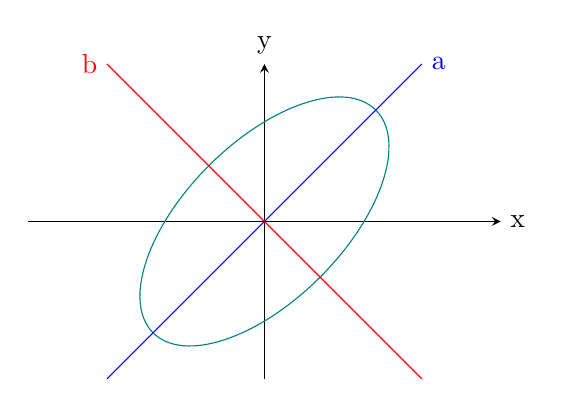
\begin{tikzpicture}[>=stealth]
\draw[->](-3,0)--(3,0)node[right]{\text{x}};
\draw[->](0,-2)--(0,2)node[above]{\text{y}};
\draw[rotate=45, teal](0,0)ellipse[x radius = 2cm, y radius =1cm];
\draw[scale=1,domain=-2:2,smooth,variable=\x,blue]plot({\x},{\x})node[right]{\text{a}};
\draw[scale=1,domain=2:-2,smooth,variable=\x,red]plot({\x},{-\x})node[left]{\text{b}};
\end{tikzpicture}
\end{figure}
\end{solution}

























\begin{exa}
Identify the quadratic surface $7x^2+7y^2+10z^2-2xy-4xz+4yz=24$\\\\
\end{exa}
\begin{solution}
$
\begin{pmatrix}
7&-1&-2\\-1&7&2\\-2&2&10\\
\end{pmatrix}
\hspace{0.4cm} \implies \lambda =6,6,12$
\begin{align*}
D(a,b,c) &=6a^2+6b^2+12c^2=24\\
         &\implies \frac{a^2}{4}+\frac{b^2}{4}+\frac{c^2}{\sqrt{2}}=1\\\\
         &\implies \frac{a^2}{2^2}+\frac{b^2}{2^2}+\frac{c^2}{\sqrt{2}}=1
\end{align*}
$\implies$ Ellipsoid.
\end{solution}

\subsection*{Practice Problems}
\addcontentsline{toc}{subsection}{Practice Problems}

\begin{problem}
Write the quadratic form $Q(x,y)=5x^2+4xy+2y^2$ in the form $x^tAx$ with $A$
symmetric, and find an orthogonal substitution reducing it to a diagonal form.
\end{problem}
\begin{solution}
\subhead{The matrix}
The coefficient of $x^2$ goes in position $(1,1)$, that of $y^2$ in $(2,2)$,
and the cross coefficient is \emph{split equally} between the two off-diagonal
positions so that the matrix is symmetric:
$$A=\begin{pmatrix}5&2\\2&2\end{pmatrix},\qquad
Q(x,y)=\begin{pmatrix}x&y\end{pmatrix}
\begin{pmatrix}5&2\\2&2\end{pmatrix}
\begin{pmatrix}x\\y\end{pmatrix}.$$

\subhead{Diagonalizing}
$$X_A(\lambda)=\begin{vmatrix}5-\lambda&2\\2&2-\lambda\end{vmatrix}
=(5-\lambda)(2-\lambda)-4=\lambda^2-7\lambda+6=(\lambda-6)(\lambda-1),$$
so the eigenvalues are $6$ and $1$. Solving $(A-6I)v=0$ gives the eigenvector
$(2,1)$; solving $(A-I)v=0$ gives $(-1,2)$. As the theory predicts for a
symmetric matrix, these are orthogonal: $(2)(-1)+(1)(2)=0$.

Normalising each to unit length and using them as columns,
$$P=\frac{1}{\sqrt5}\begin{pmatrix}2&-1\\1&2\end{pmatrix},$$
which is orthogonal, since its columns are orthonormal. Then
$$P^tAP=\begin{pmatrix}6&0\\0&1\end{pmatrix},$$
and the substitution $\begin{pmatrix}x\\y\end{pmatrix}=P\begin{pmatrix}u\\v\end{pmatrix}$
turns the form into
$$Q=6u^2+v^2,$$
with no cross term. Since both coefficients are positive, $Q$ is positive
definite and the curve $Q=1$ is an ellipse.
\end{solution}

\begin{problem}
Identify the conic $3x^2+2xy+3y^2=8$ by reducing it to diagonal form.
\end{problem}
\begin{solution}
The matrix of the form is
$A=\begin{pmatrix}3&1\\1&3\end{pmatrix}$, with
$$X_A(\lambda)=(3-\lambda)^2-1=\lambda^2-6\lambda+8=(\lambda-4)(\lambda-2),$$
so the eigenvalues are $4$ and $2$, with orthogonal eigenvectors $(1,1)$ and
$(-1,1)$ respectively. Normalising,
$$P=\frac{1}{\sqrt2}\begin{pmatrix}1&-1\\1&1\end{pmatrix},$$
which is a rotation through $45^{\circ}$. Under $x=Pu$ the equation becomes
$$4u^2+2v^2=8,\qquad\text{that is}\qquad \frac{u^2}{2}+\frac{v^2}{4}=1.$$
This is an \textbf{ellipse}, with semi-axes $\sqrt2$ along the $u$-axis and
$2$ along the $v$-axis --- the original axes rotated by $45^{\circ}$.

Because $P$ is orthogonal the substitution is a genuine rotation, so these
lengths are the true semi-axes of the original curve and not an artefact of the
change of variable.
\end{solution}

\begin{problem}
A real quadratic form $Q(x)=x^tAx$ in $n$ variables is called \emph{positive
definite} if $Q(x)>0$ for every $x\neq 0$. Show that $Q$ is positive definite
if and only if every eigenvalue of $A$ is positive.
\end{problem}
\begin{solution}
By the spectral theorem there is an orthogonal $P$ with
$P^tAP=D=\text{diag}(\lambda_1,\dots,\lambda_n)$. Substituting $x=Py$,
$$Q(x)=y^tDy=\lambda_1y_1^2+\cdots+\lambda_ny_n^2,$$
and because $P$ is invertible, $x$ ranges over all non-zero vectors exactly as
$y$ does.

\subhead{If every $\lambda_i>0$}
Then for $y\neq 0$ at least one $y_i\neq 0$, so the sum
$\sum_i\lambda_iy_i^2$ has a strictly positive term and no negative ones, hence
$Q>0$.

\subhead{If some $\lambda_k\leq 0$}
Take $y$ to be the $k$-th standard basis vector, so $y\neq 0$ and
$Q=\lambda_k\leq 0$. Then $x=Py\neq 0$ gives $Q(x)\leq 0$, so $Q$ is not
positive definite.

This is what was being checked by hand in the Section~7 problem on the value of
$c$: completing the square there was a two-variable version of the same
diagonalization.
\end{solution}

\begin{problem}
Determine whether $Q(x,y,z)=2x^2+2y^2+3z^2-2xy$ is positive definite.
\end{problem}
\begin{solution}
The symmetric matrix of the form, splitting the $-2xy$ term equally, is
$$A=\begin{pmatrix}2&-1&0\\-1&2&0\\0&0&3\end{pmatrix}.$$
Because the matrix is block diagonal, the characteristic polynomial factors:
$$X_A(\lambda)=(3-\lambda)\left[(2-\lambda)^2-1\right]
=(3-\lambda)(\lambda-1)(\lambda-3),$$
so the eigenvalues are $3$, $3$ and $1$ --- all positive. By the previous
problem $Q$ is \textbf{positive definite}.

The conclusion can be confirmed without eigenvalues by completing the square:
$$2x^2-2xy+2y^2+3z^2=2\left(x-\tfrac{y}{2}\right)^2+\tfrac{3}{2}y^2+3z^2,$$
a sum of terms with positive coefficients which vanish together only when
$z=0$, $y=0$ and then $x=0$.
\end{solution}

\pagebreak

\section*{Further reading}
\addcontentsline{toc}{section}{Further reading}
These are the texts the course was built against. They are recommendations for
a reader who wants a second treatment, not sources these notes reproduce.
\begin{enumerate}
\item A.~O. Morris, \emph{Linear Algebra: An Introduction}, 2nd edition. Van
      Nostrand Reinhold, London, 1982.
\item W.~H. Freeman, \emph{Introduction to Matrices and Linear
      Transformations}, 2nd edition, 1966.
\item D.~C. Lay, \emph{Linear Algebra and Its Applications}, 3rd edition.
      Pearson Education, Boston, 2006.
\item D.~C. Murdoch, \emph{Linear Algebra for Undergraduates}. Addison-Wesley,
      New York, 1957.
\end{enumerate}

\end{document}